\documentclass[12pt, a4paper]{article}
\pagestyle{plain}
\setlength{\parindent}{0in}
\setlength{\parskip}{2mm}

\usepackage{geometry}
% \geometry{bindingoffset=4cm}
\geometry{bindingoffset=0cm}

%%%%%%%%%%%%%%%%%%%%%%%%%%%%%
% PACKAGES & ENVIRONMENTS
%%%%%%%%%%%%%%%%%%%%%%%%%%%%%

% \usepackage[margin=0.75in]{geometry}   % Put this in each specific document to choose margin

\usepackage{amssymb,amsmath,amsthm}
\usepackage{makeidx}
%\usepackage{MnSymbol}
\usepackage{latexsym}
\usepackage{enumerate}
\usepackage{hyperref}		%% For URLs
% \usepackage{calrfsf}		%% For scroll font \mathscr{}
%\usepackage{todonotes}		%% For \todo{} margin notes
\usepackage{tikz}

\theoremstyle{definition}  %% Use non-italic text for body of Theorem


\newtheorem{Definition}{Definition}
\newtheorem{Corollary}{Theorem}
\newtheorem{Theorem}{Theorem}
\newtheorem*{Proof}{Proof}
\newtheorem{Lemma}{Lemma}
\newtheorem{Example}{Example}


% \usepackage{delarray}

%\usepackage[all,cmtip,2cell]{xy}
%\UseAllTwocells
%\input xy
%\xyoption{all}
%\xyoption{v2}

%%%%%%%%%%%%%%%%%%%%%%%%%%%%%
% STANDARD NEW COMMANDS
%%%%%%%%%%%%%%%%%%%%%%%%%%%%%

\newcommand{\upwedge}{\wedge}
\newcommand{\downwedge}{\vee}
\newcommand{\glb}{\wedge}
\newcommand{\lub}{\vee}


\newcommand{\tstile}{\vdash}
\newcommand{\makestrue}{\models}

\newcommand{\andalso}{,\;}		%% Comma with more space, for premises


% \newcommand{\newIdea}[1]{\emph{#1}} %% Emphasis for the first intro of new terminology
\newcommand{\newIdea}[1]{\textbf{#1}} %% Bold text for the first intro of new terminology
\newcommand{\terminology}[1]{\textbf{#1}} %% Bold text for the first intro of new terminology
\newcommand{\pr}[1]{\ensuremath{{#1}^{\prime}}}

\newcommand{\cat}[1]{\ensuremath{\mathcal{#1}}}
\newcommand{\category}[1]{\ensuremath{\mathcal{#1}}}
\newcommand{\Sets}{{\textsc{Sets}}}

\newcommand{\following}{\circ}

\renewcommand{\emptyset}{\varnothing}  %% Use the nice symbol
% \newcommand{\Hom}[1]{\ensuremath{\mbox{\textup{Hom}}_{#1}}}
% \newcommand{\Nat}{\mbox{\textup{Nat}}}
\newcommand{\Id}[1]{\ensuremath{\mbox{\textup{Id}}_{#1}}}
\newcommand{\monoidunit}[1]{\ensuremath{\mathbf{1}_{#1}}}
% \newcommand{\nt}{natural transformation}
% \newcommand{\NT}{Natural transformation}

%% Numbers:
\newcommand{\CC}{\ensuremath{\mathbb{C}}} %% Complex numbers
\newcommand{\RR}{\ensuremath{\mathbb{R}}} %% Real numbers
\newcommand{\QQ}{\ensuremath{\mathbb{Q}}} %% Rational numbers
\newcommand{\NN}{\ensuremath{\mathbb{N}}} %% Natural numbers
\newcommand{\ZZ}{\ensuremath{\mathbb{Z}}} %% Integers
\newcommand{\BB}{\ensuremath{\mathbb{B}}} %% Booleans

\newcommand{\HomSet}[2]{\ensuremath{\{{#1} \to {#2}\}}}

%% Logical notation:
\newcommand{\AND}{\,\&\,}
\newcommand{\OR}{\vee}
\newcommand{\NOT}{\neg}
\newcommand{\IMPLIES}{\Rightarrow}
\newcommand{\ABSURDITY}{\bot}
\newcommand{\intersect}{\cap}
\newcommand{\union}{\cup}
\newcommand{\iso}{\cong}

\newcommand{\set}[1]{\ensuremath{
\{ #1 \}
}}  %% Curly brackets for sets
\newcommand{\setSuchThat}[2]{\ensuremath{
\{ #1 \,|\, #2 \}
}}  %% Curly brackets with 'pipe' divider for sets with conditions


\newcommand{\List}[1]{\texttt{List(}#1\texttt{)}}
%\newcommand{\List}[1]{\texttt{[}#1\texttt{]}}
\newcommand{\Nil}{\texttt{[\;]}}
\newcommand{\ListOf}[2]{
\texttt{[}
#1
\texttt{||}
#2
\texttt{]}
}

\newcommand{\BTree}[1]{\texttt{BTree(}#1\texttt{)}}



% %% Some type-theory notation
\newcommand{\mono}[1]{\texttt{#1}}
% \newcommand{\term}[1]{\texttt{\ensuremath{#1}}}
\newcommand{\term}[1]{\texttt{#1}}
% \newcommand{\type}[1]{\texttt{\ensuremath{#1}}}
\newcommand{\type}[1]{\texttt{#1}}

\newcommand{\DefinedAs}{:\equiv}

%\newcommand{\TermOfType}[2]{\term{#1}:\type{#2}}
%\newcommand{\ToT}[2]{\term{#1}:\type{#2}}		%% ToT = TermOfType

%\newcommand{\IdMathrm}{\mathrm{Id}}
\newcommand{\Identity}[2]{#1 \! = \! #2}
\newcommand{\IdType}[3]{#1 \! =_{#3}\! #2}
\newcommand{\ii}{\iota}
\newcommand{\pind}[1]{\texttt{pind}_{#1}}

\newcommand{\s}{\term{s}}					% successor in \NN
\newcommand{\zN}{\term{0}_{\type{\NN}}}		% zero of \NN
\newcommand{\N}[1]{\term{#1}_{\type{\NN}}}  % numerals of \NN

\newcommand{\fin}[2]{\term{#1}_{\term{#2}}}


\newcommand{\JEqTerms}[3]{\ensuremath{\term{#1} \!\equiv\! \term{#2}:\type{#3} }}
\newcommand{\JEqTypes}[2]{\ensuremath{\type{#1} \!\equiv\! \type{#2}}}

\newcommand{\ctx}{\,\textrm{ctx}}

\newcommand{\PROD}[2]{\ensuremath{\prod_{#1} #2}}
\newcommand{\SUM}[2]{\ensuremath{\sum_{#1} #2}}
\newcommand{\AltPROD}[2]{\ensuremath{\langle{#1}\rangle \to #2}}
\newcommand{\AltSUM}[2]{\ensuremath{\langle{#1}\rangle \x #2}}
\newcommand{\TYPE}{\type{TYPE}}

%\newcommand{\PType}[2]{\type{#1}\,\ensuremath{\times}\,\type{#2}}
%\newcommand{\CType}[2]{\type{#1}\,\ensuremath{+}\,\type{#2}}
%\newcommand{\FType}[2]{\type{#1}\,\ensuremath{\to}\,\type{#2}}

\newcommand{\x}{\times}
\newcommand{\+}{+}
\newcommand{\z}{\type{0}}

\newcommand{\rec}[1]{\ensuremath{\texttt{rec}_{#1}}}
\newcommand{\ind}[1]{\ensuremath{\texttt{ind}_{#1}}}


\newcommand{\inl}{\texttt{inl}}
\newcommand{\inr}{\texttt{inr}}

\newcommand{\refl}[1]{\ensuremath{\textrm{refl}_{#1}}}

%%%%%%%%%%%%%%%%%%%%%%%%%%%%%
% DIAGRAM TEMPLATES
%%%%%%%%%%%%%%%%%%%%%%%%%%%%%

% A shortcut to make commutative squares: single-spaced
\newcommand{\SmallCommutativeSquare}[8]{
% Usage: \SmallCommutativeSquare{Top Left Object}{Top Right Object}{Bottom Left Object}{Bottom Right Object}{Top Arrow}{Left Arrow}{Right Arrow}{Bottom Arrow}
\xymatrix{
{#1} \ar[r]^{{#5}} \ar[d]_{{#6}} & {#2}\ar[d]^{{#7}} \\
{#3} \ar[r]_{{#8}}& {#4}
}
}

% A shortcut to make commutative squares: double-spaced
\newcommand{\LargeCommutativeSquare}[8]{
% Usage: \LargeCommutativeSquare{Top Left Object}{Top Right Object}{Bottom Left Object}{Bottom Right Object}{Top Arrow}{Left Arrow}{Right Arrow}{Bottom Arrow}
\xymatrix{
{#1} \ar[rr]^{{#5}} \ar[dd]_{{#6}} && {#2}\ar[dd]^{{#7}} \\
\\
{#3} \ar[rr]_{{#8}}&& {#4}
}
}


% A shortcut to make ``tent diagrams'' for natural transformations
\newcommand{\NatTransDiag}[9]{
% Usage: \NatTransDiag{Object 1}{Object 2}{Arrow}{Functor 1}{Functor 2}{Category 1}{Category 2}{NT Name}{Curvature of arrows}
\xymatrix{
&{#1} \ar[rrr]^{{#3}} \ar@/^{#9}/[ddddr]^{{#5}} \ar@/_{#9}/[dddl]_{{#4}} &&&{#2}\ar@/^{#9}/[ddddr]^{{#5}}\ar@/_{#9}/[dddl]_{{#4}}  &&& {#6} \ar@{-->}[dddd]^{{#4},\, {#5}}\\
\\
\\
{#4}({#1})\ar[drr]^{{#8}_{#1}} \ar@{->}[rrr]^{{#4}({#3})}	&&&	{#4}({#2})\ar[drr]^{{#8}_{#2}}  \\
&&	{#5}({#1})\ar[rrr]_{{#5}({#3})} 	&&&	{#5}({#2}) && {#7}
}}



% A shortcut to make ``constraint diagrams'' for natural transformations
\newcommand{\NTConstraint}[6]{
% Usage: \NTConstraint{NT Name}{Functor 1}{Functor 2}{Object 1}{Object 2}{Arrow}
\LargeCommutativeSquare
{{#2}({#4})}	% Top Left Object
{{#2}({#5})}	% Top Right Object
{{#3}({#4})}	% Bottom Left Object
{{#3}({#5})}	% Bottom Right Object
{{#2}({#6})}	% Top Arrow
{{#1}_{#4}}		% Left Arrow
{{#1}_{#5}}		% Right Arrow
{{#3}({#6})}	% Bottom Arrow
}




%%%%%%%%%%%%%%%%%%%%%%%%%%%%%
% Putting date \& time, section number into header of every page
%%%%%%%%%%%%%%%%%%%%%%%%%%%%%
\usepackage{fancyhdr, datetime}
\setlength{\headheight}{15.2pt}
\renewcommand{\headrulewidth}{0.25pt}
\renewcommand{\footrulewidth}{0pt}
\pagestyle{fancy}
\fancyhf{}
\lhead{DRAFT: \currenttime, \today }
\rhead{Section \thesubsection}
\cfoot{\thepage}
%%%%%%%%%%%%%%%%%%%%%%%%%%%%%




%%%%%%%%%%%%%%%%%%%%%%%%%%%%%
\author{Stuart Presnell \& James Ladyman
\\stuart.presnell@bristol.ac.uk
\\james.ladyman@bristol.ac.uk
}
\title{A Primer on \\Homotopy Type Theory
\\ (version 2.13)
}
% \institute[Bristol]{
  % Department of Philosophy\\
  % University of Bristol\\
  % Cotham House, Bristol BS6 6JL\\[1ex]
  % \texttt{stuart.presnell@bristol.ac.uk}
% }
%%%%%%%%%%%%%%%%%%%%%%%%%%%%%

\begin{document}
\maketitle
\begin{abstract}
A brief introduction to Homotopy Type Theory and some of the associated ideas.

The original source for the ideas presented here is the ``HoTT Book'' -- \emph{Homotopy Type Theory: Univalent Foundations of Mathematics} published by The Univalent Foundations Program, Institute for Advanced Study, Princeton.\footnote{
Page numbers for the HoTT book refer to the edition on Google Books, available at 
\href{http://books.google.co.uk/books?id=LkDUKMv3yp0C}{http://books.google.co.uk/books?id=LkDUKMv3yp0C}.
However, the book is being continually corrected and updated.  The latest edition (last updated on September 21st 2013 at the time of writing this document) is available at 
\href{http://homotopytypetheory.org/book/}{http://homotopytypetheory.org/book/}.
}  
However, the exposition in that book is rather dense and fast, whereas these notes are more gently paced for the beginner and also do more to motivate, justify, and explain things in more detail, and also address foundational and philosophical issues that the book does not.  In later sections we also go through a number of worked examples that are not covered in the book.
\end{abstract}

\newpage
\setcounter{tocdepth}{2}
\tableofcontents

\newpage



\input{Sections-1-4}
%\newpage


%\setcounter{section}{4}	%% intended section number - 1
%\section{Doing Logic in Type Theory}
\label{sec:DoingLogic}

We've now set up enough machinery to do some simple logical deductions in our type theory.  In this section we'll get some experience of using it by investigating some classical theorems to see how we prove them in HTT.  As we'll see, some proofs that are classically valid cannot be replicated in constructive logic -- they are not \terminology{constructively valid}.  We therefore need to take a little care when reasoning, in order to ensure that we're not relying on habitual moves from classical reasoning that are no longer allowed in constructive logic.  By checking a few examples we'll eventually build up a `library' of constructively valid moves that we can depend upon, which will simplify future proofs.  

Part of the goal of this section is to illustrate and reinforce the interpretation of terms and types that has been used throughout the previous sections, namely that types correspond to propositions and terms correspond to witnesses to propositions.  This way of thinking about logic is useful because the constructive logic we're using follows very naturally from it, as we saw in Section~\ref{}.  It is therefore easier to re-train our intuitions about logical reasoning from classical to constructive thinking if we use this model.  It will also be helpful when we come to introduce new elements into our type theory, such as \emph{quantifiers} and \emph{identity types}, since it's easier to understand them and motivate their definitions in this explicitly semantic terms-as-witnesses model.

Of course we could define purely \emph{syntactic} rules (as in Natural Deduction, for example) and express all our proofs as formal manipulations of expressions.  While this would serve to show which proofs are constructively valid and which are not, it would provide no experience of thinking about proofs as manipulations of witnesses to propositions.  In the following proofs we will therefore work in a \emph{semantic} mode, using the language of ``being given witnesses'' and ``constructing witnesses''.  For a formal deduction system using introduction and elimination rules, see Appendix A.2 of the Hott Book.

%
%An argument of this form constitutes an \emph{informal proof} of the proposition, in the sense of an argument that convinces mathematicians, just like the informal proofs that are published in mathematics papers with arguments stated in English.  However, in HTT we can take a further step: if we wish we can go on to make that argument completely formal -- turning an argument of the form ``given $X$ we can construct $Y$'' into a specific \emph{function} that implements this construction.  In practice we'll probably only want to complete this formalisation if we intend to have our proof automatically verified by a computer.  But the fact that we really can formalise our proof -- not just in an `in principle' kind of way, but actually in practice -- provides an extra level of reassurance that we've got it right when absolute mathematical certainty is required.



\subsection{Notation}
\label{sec:DoingLogic-Notation}

Let's first set out some notation.  To illustrate the translation into type theory notation, we'll write each example in two forms: first using the familiar ``logical notation'' ($\AND$, $\OR$, $\IMPLIES$, and $\NOT$) and then in the language of the Simple Type Theory defined in the previous section ($\x$, $\+$, $\to$, and $\to \z$).

\begin{samepage}
The theorems to be proved will be of the form ``if $Q$ and $R$ then $P$'', which we'll write as:
\[
Q\andalso R \tstile P
\]
or as simply $\tstile P$ if the theorem is a tautology involving no premises.
\end{samepage}

The translation of these into type theory will usually be written in the same way:
\[
\type{Q}\andalso \type{R} \tstile \type{P}
\] 
(and $\tstile \type{P}$ for tautologies).  However, in our constructive type theory these should be read as ``given a term of type \type{Q} and a term of type \type{R}, we can construct a term of type \type{P}''.  It will often be useful to have names for these terms that we can use in the body of the proof, so we will sometimes write the theorems as
\[
\term{q}:\type{Q}\andalso \term{r}:\type{R} \tstile \term{p}:\type{P}
\] 
Sometimes we'll only name the terms we need to refer to.  When we have terms of negation types like $\type{A} \to \z$ we'll often use the convention of naming them with an overbar, e.g. 
$\bar{\term{a}}: \type{A} \to \z$.  Similarly, terms of double negation types like 
$(\type{A} \to \z) \to \z$ will sometimes be given names with double overbars, e.g. $\bar{\bar{\term{a}}}$.

If we have $\type{A} \tstile \type{B}$ and $\type{B} \tstile \type{A}$ then we'll write 
$\type{A} \dashv \tstile \type{B}$, and sometimes (usually for comparison with another theorem) we'll write $\type{A} \tstile \type{B}$ as $\type{B} \dashv \type{A}$.

We might also want to express facts about \emph{relative constructability} -- if we can construct \type{B} from \type{A} then we can also construct \type{Y} from \type{X}.  We'll write this as
\[
\frac{\type{A} \tstile \type{B}}
{\type{X} \tstile \type{Y}}
\]
So, for example, we have
\[
\frac{\type{A} \tstile \type{B} \quad \type{B} \tstile \type{C}}
{\type{A} \tstile \type{C}}
\]
As we'll see in the next section, this relative constructability notation does not add anything new -- it doesn't make our language more expressive -- since it turns out to be just a convenient notation for something we could already express without it (i.e. what in computer science would be called ``syntactic sugar'').



% \newpage
\subsection{How do we construct a term?}
\label{sec:DoingLogic-ConstructTerm}

A proof in our type theory involves the construction a term of some specified type.  We should therefore review how we construct terms of the various types we've encountered.

Sometimes we can recover the term we want from another term:
\begin{itemize}
\item We may happen to have a function available -- either given in the premises or one that we've constructed ourselves -- that returns a term of the type we want when given an appropriate input.  In that case, we have reduced the problem to producing a term of that function's input type (which may or may not be easier than the original problem). 

\item Alternatively, we may have a term of a product type available that contains as one of its components a term of the type we're looking for.  In that case, we just extract it with the appropriate projector (which is always available).  

\item Alternatively, we may have a term of a coproduct that has as one of its options a term of the type we want.  In that case, we still have work to do.  By case analysis on the coproduct, we can say that \emph{if} the term we have is from the appropriate side of the coproduct then it's the one we want.  But then we have to go on to \emph{prove} that it will be from that side and not the other.  If we can't do that, then we've reduced the problem to constructing the term we want from a term of the \emph{other} side of this coproduct (which may or may not be easier than the original problem). 
\end{itemize}

If we can't do any of these, we will have to construct the term we want ourselves:
\begin{itemize}
\item To construct a term of a product type, such as $\type{A} \x \type{B}$, we must construct terms of each of the component types, $\term{a}:\type{A}$ and $\term{b}:\type{B}$.

\item To construct a term of a coproduct type, such as $\type{A} \+ \type{B}$, we must construct a term of \emph{one} of the component types, either $\term{a}:\type{A}$ or $\term{b}:\type{B}$ -- but either will suffice.
\end{itemize}

But what about constructing a term of a function type?  Aside from the methods mentioned above, there are basically two ways to do this.  
\begin{itemize}
\item Perhaps we have two functions already available that can be composed together to produce the function we want.  That is, if we're trying to construct a function of some type 
$\type{A} \to \type{C}$, then perhaps there's some type \type{B}, and some functions 
$\term{f}:\type{A} \to \type{B}$ and
$\term{g}:\type{B} \to \type{C}$, in which case $\term{g} \following \term{f}$ gives us the function we want.
\item If we can't do that, we our remaining technique is to use the \terminology{Deduction theorem}.  
To define a function of type 
$\type{Y} \to \type{Z}$ we need to say what it does when it's given any term of type \type{Y}.  As long as we can always find something appropriate for it to do, then we've defined our function.  By this we mean that, given an arbitrary term of \type{Y}, it must be able to produce a term of \type{Z}.  

This therefore reduces the problem of producing a term of type $\type{Y} \to \type{Z}$ given some premises to the problem of producing a term of type \type{Z} given those premises along with a term of \type{Y}.
That is, if we were originally presented with the problem of proving
\[
\type{A}\andalso \type{B}\andalso \type{C} \ldots \tstile \type{Y} \to \type{Z}
\]
%(i.e. we were trying to construct a function of type $\type{Y} \to \type{Z}$ from inputs of types $\type{A}\andalso \type{B}\andalso \type{C} \ldots$) 
then the Deduction theorem reduces this to the problem of proving
\[
\type{A}\andalso \type{B}\andalso \type{C} \ldots \type{Y} \tstile \type{Z}
\]
where the term of type \type{Y} we assume given is \emph{arbitrary} -- we can't assume anything special about it (e.g. if it's a coproduct type, we can't assume that it's from one side of the coproduct rather than the other).  In the above notation, the Deduction theorem is written:
\[
\frac
{\type{A}\andalso \type{B}\andalso \type{C} \ldots \type{Y} \tstile \type{Z}
}
{\type{A}\andalso \type{B}\andalso \type{C} \ldots \tstile \type{Y} \to \type{Z}
}
\]
\end{itemize}

Note that when we are trying to derive a negated proposition $\NOT P$ from some premises, this corresponds to constructing a function of type $\type{P} \to \z$.  According to the Deduction theorem, to do this it is sufficient to add \type{P} to the premises and derive a contradiction, since we have:
\[
\frac
{\type{A}\andalso \type{B}\andalso \type{C} \ldots \type{P} \tstile \type{0}
}
{\type{A}\andalso \type{B}\andalso \type{C} \ldots \tstile \type{P} \to \type{0}
}
\]
which is exactly the constructively valid method of \emph{Reductio ad absurdum}.\footnote{
While this form of \emph{Reductio ad absurdum} is constructively valid,  the \emph{Principle of Indirect Proof} is not
: adding $\NOT P$ to the premises and deriving a contradiction doesn't give a constructive proof of $P$; rather, it gives a proof of $\NOT \NOT P$, which is constructively weaker.
}

By the Deduction theorem, whenever we have 
$\type{A} \tstile \type{B}$ 
we also have 
$\tstile \type{A} \to \type{B}$, and so whenever we prove relative constructability
\[
\frac{\type{A} \tstile \type{B}}
{\type{X} \tstile \type{Y}}
\]
this is equivalent to proving
\[
\type{A} \to \type{B}\andalso \type{X} 
\;\tstile\; 
\type{Y}
\]
Thus the relative constructability notation is just a more convenient way of expressing something we could already say without it (except in the statement of the Deduction theorem itself).  But since it is more convenient, and aligns nicely with a useful way of thinking about constructions, we will continue to use it in subsequent proofs.


% \newpage

\newpage
\subsection{Rules involving $\AND$ and $\OR$}
\label{sec:DoingLogic-ANDORrules}

Some of the basic rules of classical logic have been taken as part of the definition of the interpretation of logic into HTT, and so we already know that they hold.  Some others follow very simply from the definitions we've given.




The Introduction and Elimination rules for conjunction and disjunction were used in the definitions of the product and coproduct, and so they hold automatically:

%$\AND$-introduction
\begin{Theorem}[$\AND$-introduction]
\[
A\andalso B \tstile A \AND B 
\]
\[
\term{a}:\type{A}\andalso 
\term{b}:\type{B} 
\tstile 
\type{A} \x \type{B} 
\]\end{Theorem}
\begin{Proof}
The definition of the product type (Section~\ref{}) says that a term of $\type{A} \x \type{B}$ consists of a pair $(\term{a}, \term{b})$, where $\term{a}:\type{A}$
and
$\term{b}:\type{B}$, so $\AND$-introduction corresponds to the term constructor for product types.
\end{Proof}

%$\AND$-elimination
\begin{Theorem}[$\AND$-elimination]
\[
A \AND B \tstile A  \quad\quad\quad  A \AND B \tstile B  
\]
\[
(\term{a}\andalso \term{b}): \type{A} \x \type{B} 
\tstile 
\type{A}
  \quad\quad\quad 
(\term{a}\andalso \term{b}): \type{A} \x \type{B} 
\tstile 
\type{B} 
\]
\end{Theorem}
\begin{Proof}
These correspond to the \emph{projectors} 
$pr_1: \type{A} \x \type{B} \to \type{A}$
and
$pr_2: \type{A} \x \type{B} \to \type{B}$
(defined in Section~\ref{}) which extract the first and second component respectively from a term 
$(\term{a}, \term{b}):\type{A} \x \type{B}$.
\end{Proof}


%$\OR$-introduction
\begin{Theorem}[$\OR$-introduction]
\[
A 
\tstile 
A \OR B  
\quad\quad\quad  
B 
\tstile 
A \OR B  
\]
\[
\term{a}: \type{A}
\tstile 
\inl(\term{a}): \type{A} \+ \type{B} 
  \quad\quad\quad 
\term{b}: \type{B} 
\tstile 
\inr(\term{b}): \type{A} \+ \type{B} 
\]\end{Theorem}
\begin{Proof}
These are the term constructors in the definition of the coproduct type.
\end{Proof}


%$\OR$-elimination
\begin{Theorem}[$\OR$-elimination]
\[
A \IMPLIES Z\andalso 
B \IMPLIES Z
\tstile
A \OR B \IMPLIES Z
\]
\[
\term{g}_l:\type{A} \to \type{Z}\andalso
\term{g}_r:\type{B} \to \type{Z} 
\tstile
\term{f}:(\type{A} \+ \type{B}) \to \type{Z} 
\]
\end{Theorem}
\begin{Proof}
This is the elimination rule in the definition of the coproduct type.
\end{Proof}


Some other rules are so trivial that they can be checked immediately by the reader, and so we won't write them out here.  In particular, the reader is left to verify:
\begin{samepage}
\begin{itemize} 
%\item $\tstile A \IMPLIES A$

\item $A \AND B \dashv \tstile B \AND A$ (commutativity of conjunction)

\item $A \OR B \dashv \tstile B \OR A$  (commutativity of disjunction)

\item $(A \AND B) \AND C \dashv \tstile A \AND (B \AND C)$ (associativity of conjunction)

\item $(A \OR B) \OR C \dashv \tstile A \OR (B \OR C)$ (associativity of disjunction)

\item $A \AND A \dashv \tstile A$ (idempotence of conjunction)

\item $A \OR A \dashv \tstile A$ (idempotence of disjunction)
\end{itemize}
\end{samepage}



Now let's look at how $\AND$ and $\OR$ interact.  We'll see that the basic classical rules for their interaction -- Absorption and Distributivity -- hold constructively as well.


%Absorption1
\begin{Theorem}[Absorption1]
\[
A \OR (A \AND B) \dashv \tstile A
\]
\[
\type{A} \+ (\type{A} \x \type{B}) \dashv \tstile \type{A}
\]
\end{Theorem}
\begin{Proof}
The right-to-left direction is trivial -- this is just the injection of \type{A} into the coproduct.  For the left-to-right direction, we do case analysis on the coproduct: if we have $\inl(\term{a})$ then we have a term of \type{A}; if we have $\inr{(\term{a},\term{b})}$ then the projector $pr_1$ gives the term of \type{A}.
\end{Proof}

%Absorption2
\begin{Theorem}[Absorption2]
\[
A \AND (A \OR B) \dashv \tstile A
\]
\[
\type{A} \x (\type{A} \+ \type{B}) \dashv \tstile \type{A}
\]
\end{Theorem}
\begin{Proof}
Again, this follows by use of the projector from the product and the injection into the coproduct.
\end{Proof}



%Distributivity of $\OR$ over $\AND$
\begin{Theorem}[Distributivity of $\OR$ over $\AND$]
\[
A \OR (B \AND C) \dashv \tstile (A \OR B) \AND (A \OR C)
\]
\[
\type{A} \+ (\type{B} \x \type{C}) \dashv \tstile (\type{A} \+ \type{B}) \x (\type{A} \+ \type{C})
\]
\end{Theorem}
\begin{Proof}
For the left-to-right direction we do case analysis on the coproduct.
\begin{itemize}
\item if we have a term of \type{A} then we have left-injectors to produce terms of $(\type{A} \+ \type{B})$ and $(\type{A} \+ \type{C})$
\item if we have a term of $(\type{B} \x \type{C})$ then the projectors give us terms of \type{B} and \type{C}, and then we have right-injectors to give terms of $(\type{A} \+ \type{B})$ and $(\type{A} \+ \type{C})$.
\end{itemize}

For the right-to-left direction, we can do two simultaneous case analyses on the two coproducts, giving four possibilities.\footnote{
Alternatively we could write these as nested case analyses, first analysing the first coproduct and then, for each case of that, doing a case analysis of the second.
}
The term of the product we're given is then either $(\term{a},\term{a})$, $(\term{a},\term{c})$, $(\term{b},\term{a})$, or $(\term{b},\term{c})$  (for some terms \term{a}, \term{b}, \term{c} of the respective types).  In the first three cases we have a term of \type{A}; in the fourth case we can produce a term of $(\type{B} \x \type{C})$; so in any case we can produce a term of the required coproduct.
\end{Proof}


%Distributivity of $\AND$ over $\OR$
\begin{Theorem}[Distributivity of $\AND$ over $\OR$]
\[
A \AND (B \OR C) \dashv \tstile (A \AND B) \OR (A \AND C)
\]
\[
\type{A} \x (\type{B} \+ \type{C}) \dashv \tstile (\type{A} \x \type{B}) \+ (\type{A} \x \type{C})
\]
\end{Theorem}
\begin{Proof}
In each direction we can do case analysis on the coproduct we're given.  We always have either terms $\term{a}$ and $\term{b}$ or terms $\term{a}$ and $\term{c}$, from which we can construct the term required.
\end{Proof}







\newpage
\subsection{Rules involving $\IMPLIES$}


%Modus ponens

The correspondence between \emph{modus ponens} and function application was part of the motivation to use the Curry-Howard correspondence to incorporate logic into our type theory, and so naturally it holds by definition:

\begin{Theorem}[Modus ponens]
\[
A\andalso A \IMPLIES B \tstile B
\]
\[
\term{a}:\type{A}\andalso \term{f}:\type{A} \to \type{B} \tstile \type{B}
\]
\end{Theorem}
\begin{Proof}
Given a function $\term{f}:\type{A} \to \type{B}$ and a term $\term{a}:\type{A}$, the result of applying \term{f} to \term{a} is, by definition, a term $\term{f}(\term{a}):\type{B}$.
\end{Proof}





%Transitivity of $\IMPLIES$
\begin{Theorem}[Transitivity of $\IMPLIES$]
\label{thm:Transitivity=>}
\[
A \IMPLIES B\andalso 
B \IMPLIES C
\tstile
A \IMPLIES C
\]
\[
\term{f}:\type{A} \to \type{B}\andalso
\term{g}:\type{B} \to \type{C} 
\tstile
\term{g} \following \term{f}:\type{A} \to \type{C} 
\]
\end{Theorem}
\begin{Proof}
The function $\term{g} \following \term{f}$ is given by composing the provided functions $\term{f}$ and $\term{g}$, i.e. 
$(\term{g} \following \term{f})(\term{a}) \DefinedAs \term{g}(\term{f}(\term{a}))$.  So transitivity of $\IMPLIES$ corresponds to composition of functions.
\end{Proof}




We used Currying and Uncurrying to define functions from product types.   Uncurrying says that, given a function of type 
$\type{A} \to (\type{B} \to \type{C})$, we can define a function of type
$(\type{A} \x \type{B}) \to \type{C}$
which takes terms of the product type as its inputs.
Currying says that any function from the product type has a corresponding curried version.  

%Currying
\begin{Theorem}[Currying]
%\label{sec:DoingLogic-CurryingUncurrying}
\[
(A \AND B) \IMPLIES C 
\tstile
A \IMPLIES (B \IMPLIES C)
\]
\[
\term{f}:(\type{A} \x \type{B}) \to \type{C}
\tstile
\term{g}:\type{A} \to (\type{B} \to \type{C})
\]
\end{Theorem}
\begin{Proof}
Given \term{f} as above, how do we define \term{g}?  What function $\term{g}_{\term{a}}:\type{B} \to \type{C}$ should it return when given an $\term{a}:\type{A}$ as input?  $\term{g}_{\term{a}}$ should map any $\term{b}:\type{B}$ to $f((a,b))$.  We can therefore define $\term{g}$ as:
\[
\term{g}(\term{a})(\term{b}) \DefinedAs \term{f}((\term{a},\term{b}))
\]
\end{Proof}


%Uncurrying
\begin{Theorem}[Uncurrying]
\[
A \IMPLIES (B \IMPLIES C)
\tstile
(A \AND B) \IMPLIES C 
\]
\[
\term{g}:\type{A} \to (\type{B} \to \type{C})
\tstile
\term{f}:(\type{A} \x \type{B}) \to \type{C}
\]
\end{Theorem}
\begin{Proof}
Going in the opposite direction, if we have a function $\term{g}$ then we can define $\term{f}$ as follows: we first use the projectors to extract $\term{a}$ and $\term{b}$ from the term of $\type{A} \x \type{B}$ that it's given as input, then feed $\term{a}$ into $\term{g}$ to get some $\term{g}_{\term{a}}:\type{B} \to \type{C}$, and finally feed $\term{b}$ into $\term{g}_{\term{a}}$.  We can therefore define $\term{f}$ as:
\[
\term{f}((\term{a},\term{b}))
\DefinedAs 
\term{g}(\term{a})(\term{b}) 
%
%f((a,b)) \DefinedAs g(a)(b)
\]
\end{Proof}

For completeness we ought to prove that currying and uncurrying are inverses to each other -- i.e. if we have a function $f:\type{A} \to (\type{B} \to \type{C})$, uncurry it to get a function from the product type, and then curry this, what we get at the end is the original $\term{f}$ (and vice versa).  However, it's fairly clear by inspection that this is the case.




%Swap
\begin{Theorem}[Swapping the order of function arguments]
\label{thm:SwapFnInputs}
\[
A \IMPLIES (B \IMPLIES C)
\tstile
B \IMPLIES (A \IMPLIES C)
\]
\[
\type{A} \to (\type{B} \to \type{C})
\tstile
\type{B} \to (\type{A} \to \type{C})
\]
\end{Theorem}
\begin{Proof}
This can be proved by an application of Uncurrying, then Commutativity of Conjunction, and then Currying.
\end{Proof}



Now let's try a more complicated example, just to confirm that we can make it work.
%``{\L}ukasiewicz's axiom''
%http://en.wikipedia.org/wiki/Hilbert-style_deduction_system#cite_ref-Tarski_2-0
\begin{Theorem}[``{\L}ukasiewicz's axiom'']
\[
A \IMPLIES (B \IMPLIES C)
\tstile
(A \IMPLIES B) \IMPLIES (A \IMPLIES C)
\]
\[
\term{g}: \type{A} \to (\type{B} \to \type{C})
\tstile
\term{h}: (\type{A} \to \type{B}) \to (\type{A} \to \type{C})
\]
\end{Theorem}
\begin{Proof}
By the Deduction Theorem (Section \ref{}) we have
\[
\frac{
\type{A} \to (\type{B} \to \type{C}), \type{A} \to \type{B}
\tstile
\type{A} \to \type{C}
}{
\type{A} \to (\type{B} \to \type{C})
\tstile
(\type{A} \to \type{B}) \to (\type{A} \to \type{C})
}
\]
and applying it again gives
\[
\frac{
\type{A} \to (\type{B} \to \type{C}), \type{A} \to \type{B}, \type{A}
\tstile
\type{C}
}{
\type{A} \to (\type{B} \to \type{C}), \type{A} \to \type{B}
\tstile
\type{A} \to \type{C}
}
\]
This top line is easily proved: given a term $\term{a}:\type{A}$ and a function $\term{f}: \type{A} \to \type{B}$ we can produce $\term{f}(\term{a}):\type{B}$.  Given a function 
$\term{g}:\type{A} \to (\type{B} \to \type{C})$ we can produce 
$\term{g}(\term{a}):\type{B} \to \type{C}$, and thus 
$\term{g}(\term{a})(\term{f}(\term{a})):\type{C}$, as required.

Thus the function 
$\term{h}: (\type{A} \to \type{B}) \to (\type{A} \to \type{C})$
that we were originally required to define, given a function
$\term{g}: \type{A} \to (\type{B} \to \type{C})$, can be written as
$
\term{h} 
\DefinedAs 
[\term{f} \mapsto [\term{a} \mapsto \term{g}(\term{a})(\term{f}(\term{a}))]]
$.
\end{Proof}


\subsection{Rules involving Negation}


Since the type corresponding to  $\NOT P$ is just the function type $\type{P} \to \z$, many of the rules involving negation are just special cases of the rules involving implication that we proved above.

%Modus Tollens
\begin{Theorem}[Modus Tollens]
\label{sec:DoingLogic-ModusTollens}
\[
A \IMPLIES B\andalso
\NOT B
\tstile
\NOT A
\]
\[
\type{A} \to \type{B}\andalso
\type{B} \to \type{0}
\tstile
\type{A} \to \type{0}
\]
\end{Theorem}
\begin{Proof}
This is just an instance of function composition (Theorem \ref{thm:Transitivity=>}).
\end{Proof}


Since in constructive logic we cannot add and remove negation signs as freely as we can in classical logic, the rule of Contraposition splits into two rules, depending upon whether the consequent of the premise is negated or not.

%``Positive'' Contraposition of $\IMPLIES$
\begin{Theorem}[``Positive'' Contraposition of $\IMPLIES$]
\[
A \IMPLIES B
\tstile
\NOT B \IMPLIES \NOT A
\]
\[
\type{A} \to \type{B}
\tstile
((\type{B} \to \z) \to (\type{A} \to \z))
\]
\end{Theorem}
\begin{Proof}
An application of the Deduction Theorem (Section \ref{}) gives:
\[
\frac{
\type{A} \to \type{B}\andalso \type{B} \to \z
\tstile
\type{A} \to \z
}{
\type{A} \to \type{B}
\tstile
((\type{B} \to \z) \to (\type{A} \to \z))
}
\]
and the first line follows by function composition.


%
%We define \term{g} as $\term{g}(\bar{\term{b}}) \DefinedAs \bar{\term{b}} \following \term{f}$.
\end{Proof}


%``Negative'' Contraposition of $\IMPLIES$
\begin{Theorem}[``Negative'' Contraposition of $\IMPLIES$]
\[
A \IMPLIES \NOT B
\tstile
B \IMPLIES \NOT A
\]
\[
\type{A} \to (\type{B} \to \z)
\tstile
\type{B} \to (\type{A} \to \z)
\]
\end{Theorem}
\begin{Proof}
This is an instance of swapping function inputs (Theorem \ref{thm:SwapFnInputs}).
\end{Proof}


%Contraposition of $\tstile$
\begin{Theorem}[Contraposition of $\tstile$]
\[
\frac{A \tstile B}
{\NOT B \tstile \NOT A}
\]

\[
\frac{\type{A} \tstile \type{B}}
{\bar{\term{b}}:\type{B}\to \z \tstile \bar{\term{a}}:\type{A} \to \z}
\]
\end{Theorem}
\begin{Proof}
By the Deduction theorem
\[
\frac{
\type{A} \tstile \type{B}
}{
\tstile \type{A} \to \type{B}
}
\]
and composing this function with ${\bar{\term{b}}}$ (i.e. by applying the rule of \emph{modus tollens}) we get a function $\bar{\term{a}}:\type{A} \to \z$.
%
%To define $\bar{\term{a}}$ we need to say what it does for any input $\term{a}:\type{A}$.  
%Since we have $\type{A} \tstile \type{B}$, we know that 
%a term $\term{b}:\type{B}$ can be constructed from $\term{a}$.
%Then since we're given $\bar{\term{b}}:\type{B}\to \z$ as a premise we simply apply it 
%%$\bar{\term{b}}$ 
%to this $\term{b}$ to get 
%$\bar{\term{b}}(\term{b}):\z$, which is then the output of $\bar{\term{a}}$.
\end{Proof}

%Non-Contradiction
The Principle of Non-Contradiction was one of our guides in defining negation, and is easily verified:

\begin{Theorem}[Non-Contradiction]
\label{thm:Non-Contradiction}
\[
\tstile
\NOT (P \AND \NOT P)
\]
\[
\tstile
\type{P}\x(\type{P}\to\z) \to \z
\]
\end{Theorem}
\begin{Proof}
A term of $\type{P} \x (\type{P}\to\z)$ is a pair 
$(\term{p}:\type{P}, 
\bar{\term{p}}:\type{P} \to \z)$.
So by function application, we have
$\bar{\term{p}}(\term{p}): \z$ by definition.  That is, non-contradiction becomes an instance of \emph{modus ponens}.
\end{Proof}


Although the Law of Excluded Middle does not hold as a rule in our constructive logic, this does \emph{not} mean that we actively \emph{deny} the validity of that rule -- we do not assert of any particular proposition $P$ that $\NOT(P \OR \NOT P)$ holds of it.  Indeed, we can prove that it is \emph{contradictory} to do so.
%\footnote{
%In the language of ``paracomplete'' logics, we do not assert that any particular $P$ is ``gappy'' (i.e. fails to have a truth value).
%}  
%Double Negation of LEM
\begin{Theorem}[Double Negation of LEM]
\label{thm:NOT-NOT-LEM}
\[
\tstile \; 
\NOT \NOT (P \OR \NOT P)
\]
\[
\tstile \; 
((\type{P} \+ (\type{P} \to \z)) \to \z) \to \z
\]
\end{Theorem}
\begin{Proof}
By the Deduction theorem, 
\[
\frac{
(\type{P} \+ (\type{P} \to \z)) \to \z
\;\;\tstile \;\;
 \z
}{
\tstile \;\;
((\type{P} \+ (\type{P} \to \z)) \to \z) \to \z
}
\]
So all that remains is to prove the top line.
From a function
$\term{f}:(\type{P} \+ (\type{P} \to \z)) \to \z$ we can derive a function 
%$\bar{\term{p}}$defined as
$\bar{\term{p}} \DefinedAs
\term{f} \following \inl$ of type $\type{P} \to \z$.  
Similarly, we can define 
$\bar{\bar{\term{p}}} \DefinedAs
\term{f} \following \inr$ of type $(\type{P} \to \z) \to \z$.  But we can then apply $\bar{\bar{\term{p}}}$ to 
$\bar{\term{p}}$ to get 
$\bar{\bar{\term{p}}}(\bar{\term{p}}):\z$.



%From the premise of the top line we will derive a witness to $(\NOT P \AND \NOT \NOT P)$, which is contradictory.



\end{Proof}







\subsection{The rule of Explosion and related results}

%Explosion
The rule of Explosion says that any arbitrary conclusion follows from contradictory premises.

\begin{Theorem}[Explosion]
\[
P \AND \NOT P
\tstile
A
\]
\[
(\term{p}, \bar{\term{p}}):\type{P} \x (\type{P} \to \z)
\tstile
\type{A}
\]
\end{Theorem}
\begin{Proof}
By the Principle of Non-contradiction (Theorem~\ref{thm:Non-Contradiction}) we get 
$\bar{\term{p}}(\term{p}):\z$.  From the definition of the Zero type, for any \type{A} there is a trivial function of type $\type{0} \to \type{A}$, which we will call $\term{!}_{\type{A}}$.  So 
$\term{!}_{\type{A}}(\bar{\term{p}}(\term{p})):\type{A}$.

(For a discussion on the constructive justification of Explosion, see Section~\ref{}.)
\end{Proof}


%$A \IMPLIES B$ with false $A$
\begin{Theorem}[$A \IMPLIES B$ with false $A$]
\label{thm:A=>B-FalseA}
\[
\NOT A
\tstile
A \IMPLIES B
\]
\[
\bar{\term{a}}:\type{A} \to \type{0}
\tstile
\term{f}:\type{A} \to \type{B}
\]
\end{Theorem}
\begin{Proof}
Using $\term{!}_{\type{B}}: \type{0} \to \type{B}$ from Explosion, we define 
$\term{f} \DefinedAs \term{!}_{\type{B}} \following \bar{\term{a}}$.
\end{Proof}


%$A \IMPLIES B$ with true $B$
\begin{Theorem}[$A \IMPLIES B$ with true $B$]
\label{thm:A=>B-TrueB}
\[
B
\tstile
A \IMPLIES B
\]
\[
\term{b}:\type{B}
\tstile
\term{k}_{\term{b}}:\type{A} \to \type{B}
\]
\end{Theorem}
\begin{Proof}
Since we are given $\term{b}:\type{B}$ we can define the constant function $\term{k}_{\term{b}}:\type{A} \to \type{B}$ that sends every 
$\term{a}:\type{A}$ to $\term{b}$.  (This result doesn't require Explosion, but we include it here to keep the subsequent discussion self-contained.)
\end{Proof}

These two rules are often called the \terminology{Paradoxes of the Material Conditional}, since they do not fit with our intuitive understanding of $\IMPLIES$ as an ``if \ldots then \ldots'' relation -- we can have $A \IMPLIES B$ even when there is no connection at all between the ideas expressed by the propositions $A$ and $B$.  The fact that we represent $\IMPLIES$ using functions $\type{A} \to \type{B}$, which convert witnesses of \type{A} into witnesses of \type{B}, seemed to hint that we would end up with a ``relevant logic''-style connective that requires a real connection between the antecedent and the consequent.  However, we see here that $\to$ behaves truth-functionally, just like the material conditional: we have a witness to $A \IMPLIES B$ whenever we have a witness to $B$ or a witness to $\NOT A$.  (However, as we'll see shortly, it is not constructively equivalent to the classical reformulations of the material conditional using $\AND$, $\OR$ and $\NOT$).








%Disjunctive Syllogism
\begin{Theorem}[Disjunctive Syllogism]
\[
A \OR B\andalso
\NOT A
\tstile
B
\]
\[
\type{A} \+ \type{B}\andalso
\bar{\term{a}}:\type{A} \to \type{0}
\tstile
\type{B}
\]
\end{Theorem}
\begin{Proof}
We proceed by case analysis on $\type{A} \+ \type{B}$.  We either have a term $\inl(\term{a})$ for some $\term{a}:\type{A}$, 
or a term $\inr(\term{b})$ for some $\term{b}:\type{B}$.
\begin{itemize}
\item If we have $\inl(\term{a})$ then 
$(\term{!}_{\type{B}} \following \bar{\term{a}})(\term{a})$ 
gives a term of $\type{B}$ (where $\term{!}_{\type{B}}$ is provided by Explosion).

\item If we have $\inr(\term{b})$ then we have $\term{b}:\type{B}$ as required.
\end{itemize}
Thus either way we can return a term of \type{B}.
\end{Proof}

As we noted in Section \ref{}, in the presence of $\OR$-introduction (which in our type theory is just the term constructor for coproducts), Disjunctive Syllogism and Explosion can be derive from each other.  Thus if we have doubts about the constructive justification for one then we should have the same doubts about the other -- or, alternatively, if we think one has a plausible constructive justification then we can use this to justify the other.


\newpage

\subsection{Rules involving \type{0} and \type{1}}

The Zero type is by definition uninhabited, and we can therefore never produce a term of it (unless we have inconsistent premises).  The Unit type is by definition uniquely inhabited, and so we can always produce a term of it, namely the single term $\ast:\type{1}$.  Since inhabitation of a type corresponds to truth of a proposition, these types can therefore be interpreted as corresponding to propositions that are known to be false and true respectively (but which have no content beyond this fact).  We can therefore interpret a few identities that are commonly written with $T$ and $F$ standing for generic true and false propositions.  We present a few examples:

\begin{Theorem}
\[
T \AND A = A
\]
\[
\type{1} \x \type{A} 
\;\;\dashv \tstile \;\;
\type{A}
\]
\end{Theorem}
\begin{Proof}
A term of $\type{1} \x \type{A}$ must be of the form $(\ast,\term{a})$ for some $\term{a}:\type{A}$, so from any term $(\ast,\term{a})$ we can recover $\term{a}$, and from any \term{a} we can construct $(\ast,\term{a})$.
\end{Proof}

\begin{Theorem}
\[
T \OR A = T
\]
\[
\type{1} \+ \type{A} 
\;\;\dashv \tstile \;\;
\type{1}
\]
\end{Theorem}
\begin{Proof}
The left-to-right direction is trivial, since we can always construct a term of \type{1} with no premises.  The right-to-left direction is also trivial, since we can always construct $\inl(\ast):\type{1} \+ \type{A}$.
\end{Proof}

\begin{Theorem}
\[
F \OR A = A
\]
\[
\type{0} \+ \type{A} 
\;\;\dashv \tstile \;\;
\type{A}
\]
\end{Theorem}
\begin{Proof}
The right-to-left direction is given by $\inr$.  The left-to-right direction is by case analysis: we either have the term $\term{a}:\type{A}$ we require, or else we can apply $\term{!}_{\type{A}}:\z \to \type{A}$.
\end{Proof}



\subsection{Equivalence of DNE and LEM}

Neither the rule of Double Negation Elimination nor the Law of Excluded Middle hold as rules in our constructive logic.  We can therefore sometimes prove that certain constructions are impossible by showing that \emph{if} they were possible they would enable us to prove the constructive validity of these rules.  In general we don't produce \emph{counterexamples} to invalid rules, as we do in classical logic,\footnote{
Question: What are counterexamples in constructive logic?  Heyting algebras with particular features?
}
so these proofs are the closest we can come to showing that an inference is not constructively valid.

We can write these ``constructive counterexamples'' using the relative constructability notation introduced in Section \ref{sec:DoingLogic-Notation}: we show 
$\type{A} \not\tstile \type{B}$ by proving
\[
\frac{\type{A} \tstile \type{B}
}{
(\type{P} \to \z) \to \z \tstile \type{P}}
%
\quad\quad\mbox{ or }\quad\quad
%\]
%or
%\[
\frac{\type{A} \tstile \type{B}
}{
\tstile \type{P} + (\type{P} \to \z)}
\]

We might now wonder whether a constructive counterexample that results in DNE is different from one that ends in LEM -- they both show that the inference is not constructively valid, but do they do so in essentially different ways?  In this section we will show that they are equivalent, because DNE and LEM can be proved from each other.

%LEM $\IMPLIES$ DNE
\begin{Theorem}[LEM $\IMPLIES$ DNE]
\[
\frac{
\tstile \type{P} + (\type{P} \to \z)
}{
(\type{Q} \to \z) \to \z \tstile \type{Q}
}
\]
\end{Theorem}
\begin{Proof}
If LEM holds then in particular we have 
$\tstile \type{Q} + (\type{Q} \to \z)$.  That is, from no premises we can construct something that is either a term of \type{Q} or a term of $\type{Q} \to \z$.  We then reason by case analysis to prove $(\type{Q} \to \z) \to \z \tstile \type{Q}$: we either have a term of $\type{Q}$ already, in which case there is nothing more to prove;  or we have a term of $(\type{Q} \to \z)$ in which case we apply $(\type{Q} \to \z) \to \z$ to get a contradiction, from which we can derive a term of \type{Q} by  Explosion.
\end{Proof}


%DNE $\IMPLIES$ LEM
\begin{Theorem}[DNE $\IMPLIES$ LEM]
\[
\frac{
(\type{Q} \to \z) \to \z \tstile \type{Q}
}{
\tstile \type{P} + (\type{P} \to \z)
}
\]
\end{Theorem}
\begin{Proof}
We have seen in Theorem \ref{thm:NOT-NOT-LEM} that we can constructively prove the Double Negation of LEM, $\NOT \NOT (P \OR \NOT P)$
\[
((\type{P} + (\type{P} \to \z)) \to \z) \to \z
\]
Thus by Double Negation Elimination we obtain LEM itself.
\end{Proof}


\subsection{Differences between Classical and Constructive logic}
\label{sec:DoingLogic-MoreResults}

Now we've covered the basics, let's explore some of the ways our constructive logic is similar and different from classical logic.


\subsubsection{Relationship between $A \IMPLIES B$, $(\NOT A) \OR B$, and $\NOT (A \AND \NOT B)$}

Classically, since $A \IMPLIES B$ is just a truth function, we can define it with $\AND$, $\OR$, and $\NOT$ in at least two different but logically equivalent ways, as $(\NOT A) \OR B$, and $\NOT (A \AND \NOT B)$.  How do these compare constructively?

\begin{Theorem}
\[
(\NOT A) \OR B
\tstile
A \IMPLIES B
\]
\[
(\type{A} \to \z) \+ \type{B}
\tstile
\type{A} \to \type{B}
\]
\end{Theorem}
\begin{Proof}
By case analysis: we either have a function 
$\bar{\term{a}}:\type{A} \to \z$ or a term $\term{b}:\type{B}$, and we have seen in Theorems \ref{thm:A=>B-FalseA} and \ref{thm:A=>B-TrueB} that we can construct a term of $\type{A} \to \type{B}$ from either of these.
\end{Proof}

\begin{Theorem}
\[
A \IMPLIES B
\tstile
\NOT (A \AND \NOT B)
\]
\[
\term{f}:\type{A} \to \type{B}
\tstile
\term{g}:(\type{A} \x (\type{B} \to \z)) \to \z
\]
\end{Theorem}
\begin{Proof}
We define $\term{g}:(\type{A} \x (\type{B} \to \z)) \to \z$ as
%
%
%We need to define a function \term{g} that, when given an 
%$\term{a}:\type{A}$ and a 
%$\bar{\term{b}}:\type{B} \to \z$
%returns a term of $\z$.  We can define this as
\[
\term{g}(\term{a})(\bar{\term{b}}) 
\DefinedAs 
\bar{\term{b}}(\term{f}(\term{a}))
\]
\end{Proof}


This shows that
\[
(\type{A} \to \z) \+ \type{B}
\;\;\tstile\;\;
\type{A} \to \type{B}
\;\;\tstile\;\;
(\type{A} \x (\type{B} \to \z)) \to \z
\]
However, the reverse constructions \emph{cannot} be carried out constructively: if they could, then we would have either Double Negation Elimination or the Law of Excluded Middle, which we know is not the case.  Let's prove this now.

\begin{Theorem}
\[
\frac{
\type{A} \to \type{B}
\;\;\tstile\;\;
(\type{A} \to \z) \+ \type{B}
}{
\tstile (\type{A} \to \z) \+ \type{A}
}
\]
\end{Theorem}
\begin{Proof}
If the construction on the top line can be carried out for any arbitrary types \type{A} and \type{B} then we have in particular
$\type{A} \to \type{A}
\tstile
(\type{A} \to \z) \+ \type{A}$.  But we always have the identity function 
$\type{A} \to \type{A}$, so we require no further premises in order to define it.  Thus we obtain the Law of Excluded Middle.
\end{Proof}


%\newpage
\begin{Theorem}
\[
\frac{
(\type{A} \x (\type{B} \to \z)) \to \z
\;\;\tstile\;\;
\type{A} \to \type{B}
}{
(\type{B} \to \z) \to \z
\;\;\tstile\;\;
\type{B}
}
\]
\end{Theorem}
\begin{Proof}
If the construction on the top line can be carried out for any arbitrary types \type{A} and \type{B} then we have in particular
$(\type{1} \x (\type{B} \to \z)) \to \z
\tstile
\type{1} \to \type{B}$,
where \type{1} is the Unit type.  But it is clear that
$
(\type{B} \to \z) \to \z
\tstile
(\type{1} \x (\type{B} \to \z)) \to \z
$
and
$\type{1} \to \type{B} \tstile \type{B}$.  Putting these together, we get the required conclusion, namely Double Negation Elimination.

\end{Proof}

So, constructively, these three propositions are strictly ordered in strength:  the strongest is $(\NOT A) \OR B$, 
then $A \IMPLIES B$ is intermediate in strength, and 
$\NOT (A \AND \NOT B)$ is strictly weaker than the other two.\footnote{
Also, note that we can prove 
$(\type{A} \to \z) \+ \type{B}
\tstile
(\type{A} \x (\type{B} \to \z)) \to \z$
directly without going via $\type{A} \to \type{B}$, by a case analysis on the coproduct, and that this direct construction therefore does not depend upon Explosion.
}




\subsubsection{Double Negation Introduction}

Although in constructive logic we don't have Double Negation Elimination (DNE) as a rule, we can prove Double Negation Introduction (DNI) as a theorem:
\begin{Theorem}
\label{thm:DNI}
\[
A 
\tstile 
\NOT \NOT A
\]
\[
\type{A}
\tstile 
(\type{A} \to\z)\to\z
\]
\end{Theorem}
\begin{Proof}
This follows immediately from the Deduction theorem and the Principle of Non-contradiction.
\end{Proof}

The function $\bar{\bar{\term{a}}}:(\type{A} \to\z)\to\z$ that we obtain from a given $\term{a}:\type{A}$ could be called $\term{evaluate-at-a}$, since we define 
\[
\bar{\bar{\term{a}}}(\bar{\term{a}}) \DefinedAs
\bar{\term{a}}(\term{a})
\]

%must be a function that takes any 
%$\bar{\term{a}}:\type{A} \to\z$ and returns a term of $\z$.  We can do this by evaluating 
%$\bar{\term{a}}$ at $\term{a}$.  We could therefore rename $\bar{\bar{\term{a}}}$ as 

This is directly analogous with the relationship between a vector space $V$ and its double-dual vector space $V^{\ast\ast}$.  Recall that for any vector space $V$ the dual space $V^{\ast}$ consists of linear functions $f:V\to \RR$ (or to whatever field $V$ is defined over).  Thus for any vector $v \in V$ there is an element $\hat{v} \in V^{\ast\ast}$ (i.e. a linear function $\hat{v}: V^{\ast} \to \RR$) defined by
\[
%\forall f \in V^{\ast}, 
\hat{v}(f) \DefinedAs f(v)
\]
i.e. $\hat{v}$ is like an ``evaluate at $v$'' operation.

% \newpage
%\subsubsection{Generalising DNI}
%
%\[
%A
%\tstile
%(A \IMPLIES B) \IMPLIES B
%\]
%\[
%\term{a}:\type{A}
%\tstile 
%((\type{A} \to \type{B}) \to \type{B})
%\]
%Nothing about the above proof of DNI referred to \type{0} in particular, and so the argument can immediately be generalised to any other type \type{B}.  The required function takes any $\term{f}:\type{A} \to \type{B}$ and evaluates it at the given term $\term{a}:\type{A}$ to give 
%$\term{f}(\term{a}):\type{B}$.
%
%We could again call this 
%$\term{evaluate-at-a}$, but we should be careful: this is not \emph{the same} function that we defined in the proof of DNI, since it's of a different type -- it's of type
%$((\type{A} \to \type{B}) \to \type{B})$ (for some particular \type{B})
%whereas that one was of type
%$((\type{A} \to \type{0}) \to \type{0})$.
%We can define such a function for any output type \type{Z}, of course, but because of the strictness of the type system each of these will be a different function, each one of which does the job of evaluating functions at \type{a} within its own private domain.
%
%Naturally, we want to overcome this petty distinction, since each of these functions does essentially the same thing.  We will be able to do this later\footnote{See Section~\ref{}}, when we have introduced \terminology{type polymorphism} -- then we'll be able to define a function that can take any function out of \type{A} as input and evaluate it at a given $\term{a}$.
%
%We might also wonder (restricting our attention to a particular type \type{B} for now) whether we can generalise in a different direction.
%Rather than being stuck with a particular value \term{a} at which to evaluate functions, can we define a new function that takes any term $\term{x}:\type{A}$ as input and returns the specific $\term{evaluate-at-x}$ function as output?  The answer is yes, we can.  But we won't do this now: we'll come back to this question later\footnote{Section~\ref{}}, in response to a much broader question.








%%% For more examples of constructively valid and invalid classical tautologies, see Section 9 of http://planetmath.org/intuitionisticlogic

%%% Also, run through the list of https://en.wikipedia.org/wiki/Rule_of_inference and see which hold.

%%% See also:
%%% https://en.wikipedia.org/wiki/Tautology_(logic)
%%% https://en.wikipedia.org/wiki/Axiomatization_of_Boolean_algebras#Axiomatics



\subsubsection{Triple Negation}

Although we cannot eliminate double negations \emph{in general}, this theorem shows that we can eliminate them when they occur directly in front of negated propositions.

\begin{Theorem}
\[
\NOT\NOT\NOT A
\tstile
\NOT A
\]
\[
\term{f}:((\type{A} \to \z) \to \z) \to \z
\tstile
\term{g}:\type{A} \to \z
\]
\end{Theorem}
\begin{Proof}
By the Deduction theorem, 
\[
\frac{
((\type{A} \to \z) \to \z) \to \z \andalso \type{A}
\tstile
\z
}{
((\type{A} \to \z) \to \z) \to \z
\tstile
\type{A} \to \z
}
\]
so all that remains is to prove the top line, i.e. to prove that the premises are contradictory.

We saw in Theorem \ref{thm:DNI} that from any $\term{a}:\type{A}$ we can construct $\bar{\bar{\term{a}}}: (\type{A} \to \z) \to \z$.  Thus from the premises of the top line we have 
$(\type{A} \to \z) \to \z$
and 
$((\type{A} \to \z) \to \z) \to \z$, and so by \emph{modus ponens} we have the required contradiction.
\end{Proof}


%A standard way to prove this in classical logic is to assume $A$ for proof by contradiction; derive $\NOT\NOT A$ from $A$ by DNI; then since we have both $\NOT\NOT\NOT A$ (premise) and $\NOT\NOT A$ (derived from $A$) we get a contradiction; this contradiction followed from the assumption of $A$, so we have proved $\NOT A$.  Thus $\NOT\NOT\NOT A   \tstile  \NOT A$ as required.
%
%The proof in our constructive logic is similar.  But since our aim here is to define a function 
%$\bar{\term{a}}:\type{A} \to \z$, 
%we can skip the \emph{assume $A$ for contradiction} step; to define $\bar{\term{a}}$ we need to say what it will do for any input $\term{a}:\type{A}$; thus the $\term{a}$ is \emph{provided}, not \emph{assumed}.\footnote{
%TODO: There's probably a better way to explain this.
%}
%
%So what does our \term{g} do when given an $\term{a}:\type{A}$?  We can follow the steps of the classical proof exactly.  First it uses that \term{a} to construct a term $\bar{\bar{\term{a}}}:((\type{A} \to \z) \to \z)$ by DNI; then it applies the given function \term{f} 
%to map $\bar{\bar{\term{a}}}$ to a term of $\z$ (i.e. a contradiction); this term of $\z$ is then the output.
%
%We can set out the two proofs side-by-side to see the similarity:
%
%
%\begin{table}[h]
%\centering
%\begin{tabular}{|r|l|}
%\hline
%Classical proof	&	Constructive proof\\
%\hline
%$\NOT\NOT\NOT A$ \quad [\emph{premise}]		
%&		$\term{f}:((\type{A} \to \z) \to \z) \to \z$ \quad [\emph{given}]
%
%\\
%Assume $A$ for contradiction	
%&		$\term{a}:\type{A}$ \quad [\emph{input to} \term{g}]	
%\\
%Derive $\NOT\NOT A$ from $A$ by DNI		
%&		Construct $\bar{\bar{\term{a}}}:((\type{A} \to \z) \to \z)$ from \term{a} by DNI
%\\
%$\NOT\NOT A$ and $\NOT\NOT\NOT A$ -- contradiction	
%&		Apply \term{f} to $\bar{\bar{\term{a}}}$ to get 
%$\term{f}(\bar{\bar{\term{a}}}): \z$
%\\
%$\ABSURDITY$ derived from assumption of $A$		
%&		This defines $\term{g}:\type{A} \to \z$
%\\
%$\NOT\NOT\NOT A   \tstile  \NOT A$		
%&		
%$((\type{A} \to \z) \to \z) \to \z 
%\tstile
%\type{A} \to \z$
%\\		
%\hline
%\end{tabular}
%\end{table}
%
%









%\newpage
\subsection{de Morgan's laws}
\label{sec:DoingLogic-deMorgan}

de Morgan's laws relate certain expressions involving $\AND$, $\OR$, and $\NOT$.  Since our logic is constructive logic we have to be a bit more careful around negations, and so we have more relationships to check than we would in classical logic:

\begin{table}[h]
\centering
\begin{tabular}{c c c }
$(A \AND B)$					&$\dashv \; \tstile$ 	&$\NOT(\NOT A \OR \NOT B)$ \\
$(\NOT A \AND \NOT B)$ 	 	&$\dashv \; \tstile$ 	&$\NOT(A \OR B)$ \\
$\NOT(A \AND B)$  				&$\dashv \; \tstile$ 	&$(\NOT A \OR \NOT B)$ \\
$\NOT (\NOT A \AND \NOT B)$	&$\dashv \; \tstile$ 	&$(A \OR B)$
\end{tabular}
\end{table}
These all hold classically, of course, but we must check all 8 of them to see which hold constructively and which do not.  As we'll see, for the laws that do hold the required constructions are quite  straightforward\footnote{
Despite the rather complex presentation in the HoTT Book (p. 42).
}

In each case we'll write the classical statement (for which the entailments hold in both directions) followed by the constructive version (for which, in some cases, only one direction of entailment holds).


\subsubsection{First de Morgan Law}
\begin{Theorem}[First de Morgan Law]
\[
(A \AND B)
\dashv \tstile 
\NOT(\NOT A \OR \NOT B)
\]
\[
(\term{a},\term{b}):(\type{A} \x \type{B})
\not\dashv \tstile 
\term{g}:((\type{A} \to \z) \+ (\type{B} \to \z)) \to \z
\]
\end{Theorem}
\begin{Proof}
$\tstile$: Given $\term{a}:\type{A}$ and $\term{b}:\type{B}$ we can define the function \term{g} by case analysis on its input: if its input is a term of $\type{A} \to \z$ then it applies this to \term{a}, whereas if its input is a term of $\type{B} \to \z$ then it applies this to \term{b}.

$\not\dashv$: This direction is not constructively valid: if we could carry out this construction then we could use it to prove that DNE is constructively valid:

\begin{Lemma}
\[
\frac{
((\type{A} \to \z) \+ (\type{B} \to \z)) \to \z
\;\;\tstile \;\;
\type{A} \x \type{B}
}{
(\type{A} \to \z) \to \z
\;\; \tstile \;\; 
\type{A}
}
\]
\end{Lemma}
\begin{Proof}
If the top line holds for arbitrary types \type{A} and \type{B} then in particular we have 
\[
((\type{A} \to \z) \+ (\type{1} \to \z)) \to \z
\;\;\tstile \;\;
\type{A} \x \type{1}
\]
It is then a simple matter to see that the left side of the turnstile is equivalent to $(\type{A} \to \z) \to \z$, while the right side is equivalent to $\type{A}$.
\end{Proof}
Thus, since DNE is \emph{not} constructively valid, nor is this direction of the First de Morgan Law.

\end{Proof}



\subsubsection{Second de Morgan Law}
\begin{Theorem}[Second de Morgan Law]
\[
(\NOT A \AND \NOT B)
\dashv \tstile
\NOT(A \OR B)
\]
\[
(\bar{\term{a}}, \bar{\term{b}}):((\type{A} \to \z) \x (\type{B} \to \z))
\dashv \tstile 
\term{g}:(\type{A} \+ \type{B}) \to \z
\]\end{Theorem}
\begin{Proof}
$\tstile$: Given $\bar{\term{a}}:\type{A} \to \z$ and $\bar{\term{b}}:\type{B} \to \z$, we define the function \term{g} by case analysis: it applies either $\bar{\term{a}}$ or $\bar{\term{b}}$ to its input.

$\dashv$: Given a function $\term{g}:(\type{A} \+ \type{B}) \to \z$, we define $\bar{\term{a}}:\type{A} \to \z$ and $\bar{\term{b}}:\type{B} \to \z$ as follows:
\[
\bar{\term{a}} \DefinedAs \term{g} \following \inl \quad \quad
\bar{\term{b}} \DefinedAs \term{g} \following \inr
\]
(Note that this is a generalisation of the technique we used in Theorem \ref{thm:NOT-NOT-LEM}.)
\end{Proof}



\subsubsection{Third de Morgan Law}
\begin{Theorem}[Third de Morgan Law]
\[
\NOT(A \AND B)
\dashv \tstile 
(\NOT A \OR \NOT B)
\]
\[
\term{f}:(\type{A} \x \type{B}) \to \z
\dashv \not\tstile 
%\term{g}:
((\type{A} \to \z) \+ (\type{B} \to \z))
\]
\end{Theorem}
\begin{Proof}
$\not\tstile$: This direction is not constructively valid.
The function \term{f} can only be applied to pairs $(\term{a}, \term{b})$.  From this, we cannot construct a function $\type{A} \to \z$, since we have no way of creating an element of an arbitrary type \type{B} given only a term of \type{A} as input.  Likewise, we can't construct a function $\type{B} \to \z$.  Thus we cannot construct a term of the coproduct
$((\type{A} \to \z) \+ (\type{B} \to \z))$.

$\dashv$: By case analysis we either have a term $\bar{\term{a}}:\type{A} \to \z$ or a term $\bar{\term{b}}:\type{B} \to \z$, and either of these is sufficient to construct a function $(\type{A} \x \type{B}) \to \z$.  
If we have $\bar{\term{a}}$ we define 
$\term{f} \DefinedAs \bar{\term{a}} \following pr_1$, 
whereas
if we have $\bar{\term{b}}$ we define 
$\term{f} \DefinedAs \bar{\term{b}} \following pr_2$.
\end{Proof}






\subsubsection{Fourth de Morgan Law}
\begin{Theorem}[Fourth de Morgan Law]
\[
\NOT (\NOT A \AND \NOT B)
\;\;\dashv \tstile\;\;
(A \OR B)
\]
\[
\term{f}:((\type{A} \to \z) \x (\type{B} \to \z)) \to \z
\;\;\dashv \not\tstile \;\;
\type{A} \+ \type{B}
\]
\end{Theorem}
\begin{Proof}
$\not\tstile$: This direction is not constructively valid: if we could carry out this construction then we could use it to do DNE, as follows:
\begin{Lemma}
\[
\frac{
((\type{A} \to \z) \x (\type{B} \to \z)) \to \z
\;\;\tstile \;\;
\type{A} \+ \type{B}
}{
(\type{A} \to \z) \to \z
\;\;\tstile\;\;
\type{A}
}
\]
\end{Lemma}
\begin{Proof}
If the top line holds for arbitrary types \type{A} and \type{B} then in particular we have:
\[
((\type{A} \to \z) \x (\type{0} \to \z)) \to \z
\;\;\tstile \;\;
\type{A} \+ \type{0}
\]
It is then straightforward to show that the left side of the turnstile is equivalent to $(\type{A} \to \z) \to \z$, while the right side is equivalent to $\type{A}$.
\end{Proof}

$\dashv$:  By case analysis: if we have a term $\term{a}:\type{A}$ then we define \term{f} as
\[
\term{f}((\bar{\term{a}}, \bar{\term{b}})) \DefinedAs \bar{\term{a}}(\term{a})
\]
whereas if we have a term $\term{b}:\type{B}$ then we define \term{f} as
\[
\term{f}((\bar{\term{a}}, \bar{\term{b}})) \DefinedAs \bar{\term{b}}(\term{b})
\]

\end{Proof}


\subsubsection{Summary of the Constructive de Morgan laws}

We divided the classical de Morgan laws into 8 different entailments, and we have seen that only 5 of them hold constructively:

\begin{table}[h]
\centering
\begin{tabular}{c c c }
$(A \AND B)$					&$\not\dashv \; \tstile$ 	&$\NOT(\NOT A \OR \NOT B)$ \\
$(\NOT A \AND \NOT B)$ 	 	&$\dashv \; \tstile$ 	&$\NOT(A \OR B)$ \\
$\NOT(A \AND B)$  				&$\dashv \; \not\tstile$ 	&$(\NOT A \OR \NOT B)$ \\
$\NOT (\NOT A \AND \NOT B)$	&$\dashv \; \not\tstile$ 	&$(A \OR B)$
\end{tabular}
\end{table}

Of the three that do not hold constructively, we gave explicit counterexamples for two of them, showing that if they were constructively valid then we would obtain constructive DNE as a special case.  However, for the other constructively invalid law, namely
\[
(\type{A} \x \type{B}) \to \z
\;\; \not\tstile \;\;
((\type{A} \to \z) \+ (\type{B} \to \z))
\]
we were not able to give such an argument.  We could make a plausible case that, since we cannot create arbitrary terms of arbitrary types, we cannot use a function $(\type{A} \x \type{B}) \to \z$ to construct either a function $\type{A} \to \z$ 
nor a function $\type{B} \to \z$.  But this is not as strong an argument as showing that an entailment's validity would lead to impossible results.  Can we do better than this?

If we try the obvious methods, substituting special values in for \type{A} and \type{B}, this only leads to conclusions that are constructively acceptable.  For example, if we replace \type{B} with \type{1} we get
\[
(\type{A} \x \type{1}) \to \z
\;\; \tstile \;\;
((\type{A} \to \z) \+ (\type{1} \to \z))
\]
which is easily seen to be equivalent to $\type{A} \to \z \tstile \type{A} \to \z$.  Similarly, if we replace \type{B} with $\type{A} \to \z$ we get
\[
(\type{A} \x (\type{A} \to \z)) \to \z
\;\; \tstile \;\;
((\type{A} \to \z) \+ ((\type{A} \to \z) \to \z))
\]
The left side of this always holds, so the above statement corresponds to what we might call ``the Law of Excluded Middle for Negated Propositions'' 
${\tstile \NOT A \OR  \NOT \NOT A}$, which is constructively fine.\footnote{
TO DO: Or is it?  Prove this one way or the other!
}

We therefore need a more powerful technique to demonstrate the constructive invalidity of an argument.  We introduce such a technique in the next section.




%None of the 5 constructively valid rules makes explicit reference to the involvement of the Zero type, and so none relies upon Explosion.  Moreover, we could immediately generalise them to replace $\z$ with an arbitrary type \type{Z} if we wanted, which would give some obvious (but not particularly interesting) logical rules such as:
%%
%% First Law:
%\[
%(A \AND B)
%\;\; \tstile \;\; 
%((A \IMPLIES Z) \OR (B \IMPLIES Z)) \IMPLIES Z
%\]
%\[
%(A \x B)
%\;\; \tstile \;\; 
%((A \to Z) \+ (B \to Z)) \to Z
%\]
%
%% Second Law
%% \[
%% ((A \IMPLIES Z) \AND (B \IMPLIES Z))
%% \;\;  \dashv \; \tstile \;\; 
%% (A \OR B) \IMPLIES Z
%% \]
%% \[
%% ((A \to Z) \x (B \to Z))
%% \;\;  \dashv \; \tstile \;\; 
%% (A \+ B) \to Z
%% \]
%
%% Third Law:
%% \[
%% ((A \IMPLIES Z) \OR (B \IMPLIES Z))
%% \;\; \tstile \;\; 
%% (A \AND B) \IMPLIES Z
%% \]
%% \[
%% ((A \to Z) \+ (B \to Z))
%% \;\; \tstile \;\; 
%% (A \x B) \to Z
%% \]
%
%% Fourth Law:
%% \[
%% (A \OR B)
%% \;\; \tstile  \;\; 
%% ((A \IMPLIES Z) \AND (B \IMPLIES Z)) \IMPLIES Z
%% \]
%% \[
%% (A \+ B)
%% \;\; \tstile  \;\; 
%% ((A \to Z) \x (B \to Z)) \to Z
%% \]


%
%%%%%%%%%%%%%%%%%%%%%%%%%%%%%%%%%%%%


%\newpage


%\setcounter{section}{5}	%% intended section number - 1
%\section{Models and Counter-models for Constructive logic}


In our previous investigations of constructive validity, we have shown that certain arguments are constructively valid by demonstrating specifically how to carry out those constructions.  We have also, in some cases, shown that 
if a particular argument were constructively valid then
we could use it to prove the constructive validity of DNE and LEM, which therefore demonstrates (by \emph{modus tollens}) that the argument is \emph{not} constructively valid.
However, we have not been able to do this in all cases: in particular, we could not find a way to deduce LEM from the Third de Morgan Law.  Moreover, it is not that case that all constructively invalid arguments allow us to derive constructively unacceptable conclusions like LEM and DNE.\footnote{
Specifically, classical logic is obtained by adding LEM to constructive logic, but there are \emph{intermediate logics} between constructive and classical logic which add new axioms that cannot be proved constructively but which are not as powerful as classical logic. 
}

We therefore need more powerful techniques.  In this Section we will investigate a few different approaches to demonstrating the constructive validity or invalidity of arguments, and see how they are related to one another.

%\newpage
\subsection{Truth tables and tautologies}
\label{sec:Models-TruthTables}

A standard way of establishing the validity of a formula in classical propositional logic (i.e. an expression built up from $\AND$, $\OR$, $\NOT$, $\IMPLIES$, and variables representing propositions)
is by constructing a \emph{truth table}.  Each propositional variable can be either true or false, and so for a formula involving $n$ variables there are $2^n$ possible assignments of truth values to its variables.  We can therefore work out the truth value of the formula itself under each possible assignment.  If the formula is true for every posible assignment of truth values then it is a \emph{tautology} of classical propositional logic.  A further result then shows that a formula can be proved in CPL if and only if it is a tautology.

For example, consider the third de Morgan law (or rather, the formula we get from it by applying the Deduction theorem)
\[
\NOT (P \AND Q) \IMPLIES ((\NOT P) \OR (\NOT Q))
\]
There are two propositional variables, so we have $2^2$ possible assignments of truth values to them.  In each case we can work out the truth value of the formula:\\
\begin{table}[h]
\centering
\begin{tabular}{c c|c c c}
P &	Q & $\NOT(P \AND Q)$ &	$(\NOT P) \OR (\NOT Q)$ &	$\NOT (P \AND Q) \IMPLIES ((\NOT P) \OR (\NOT Q))$ \\
\hline
T & T & F & F & T\\
T & F & T & T & T\\
F & T & T & T & T\\
F & F & T & T & T\\
\end{tabular}
\end{table}\\
The formula is true under any assignment, and so it is a classical tautology.

This procedure has the advantage that it is guaranteed either to  confirm that a formula is a tautology or to provide a \emph{counterexample} -- a particular assignment of truth values to variables under which the formula is false.  Moreover this procedure is entirely mechanical, and so a computer can check the validity of any finite formula of CPL.  Finally, if we are given a putative counterexample we can immediately verify it for ourselves by evaluating the formula with those values.  We therefore don't simply have to trust the computer program when it tells us that a formula is not a tautology.

These features are exactly what we want for our system: invalid arguments can be identified \emph{automatically}, and their invalidity is certified by a \emph{witness}, i.e. the particular counterexample.  It would therefore be useful to be able to adapt this method from classical to constructive logic.


\subsection{Boolean and Heyting algebras}

The modification of this technique that's required is conceptually simple.  The truth values we use in classical logic, $T$ and $F$, form a \terminology{Boolean algebra} -- a collection of values on which we can define the operations $\AND$, $\OR$, $\NOT$, and $\IMPLIES$, all of which behave as we expect, and which satisfies $\NOT \NOT x = x$ for all elements.  We can build up the definition of a Boolean algebra in stages.  

A \terminology{lattice} is a set of elements equipped with a preordering -- a relationship $\leq$ that is reflexive and transitive -- such that any pair of elements has both a greatest lower bound and a least upper bound.  We write the greatest lower bound of $x$ and $y$ as $x \glb y$, and the least upper bound as $x \lub y$.

A lattice is \terminology{distributive} if for all $x, y, z$ in the lattice we have
\[
x \glb (y \lub z) = (x \glb y) \lub (x \glb z)
\]
or, equivalently,
\[
x \lub (y \glb z) = (x \lub y) \glb (x \lub z)
\]
%or equivalently,
%\[
%x\wedge z = y\wedge z 
%\;\mbox{  and  }\;
% x\vee z = y\vee z 
%\;\mbox{  implies  } \;
%x=y
%\]
This allows us to give a particularly simple representation of any finite distributive lattice: we can represent it as a collection of (some of the) subsets of some finite set $S$.  The ordering relation is then given by subset inclusion, while $\glb$ and $\lub$ are given by intersection and union respectively.\footnote{This representation theorem was proved by Birkhoff (1937).
}  We can therefore use $\glb$ and $\lub$ to represent conjunction and disjunction in logic: the items in $x \glb y$ are those in both $x$ and $y$, while the items in $x \lub y$ are those in either $x$ or $y$.

A lattice is \terminology{bounded} if it has elements $1$ and $0$ such that for all elements $x$ in the lattice, $0 \leq x \leq 1$.  It is easy to confirm that $x \lub 0 = x = x \glb 1$, $x \glb 0 = 0$, and $x \lub 1 = 1$.  Every finite distributive lattice is bounded, with $S$ as $1$ and $\varnothing$ as $0$.

How do we represent implication, $x \IMPLIES y$?  Given a distributive lattice, we can consider for any $x$ and $y$ the elements $z$ such that $x \glb z \leq y$.  In the representation as subsets, these are the sets disjoint from $x \setminus y$
(where $x \setminus y$ is the set of items in $x$ but not in $y$).  That is, if an item is in such a $z$ and also in $x$, then it must be in $y$ as well.  If there is a \emph{maximal} such $z$ for a given $x$ and $y$ then we take this element to represent $x \IMPLIES y$.  

A \terminology{Heyting algebra} is a bounded distributive lattice in which for every pair $x$, $y$ there is an element 
\[
x \to y \DefinedAs \mbox{max}\setSuchThat{z}{x \glb z \leq y}
\]
In particular, in a finite distributive lattice such a maximum always exists, since the union of all such $z$ is an element of the lattice, and so every finite distributive lattice is a Heyting algebra.

In any Heyting algebra we can define $\NOT x$ as $x \to 0$ (in accordance with our definition in our constructive logic).  In the representation as subsets this is the largest subset in the lattice that is \emph{disjoint} with $x$ -- that is, it's some subset of $S \setminus x$.  However, in an arbitrary Heyting algebra $S \setminus x$ itself will not in general be an element of the lattice whenever $x$ is, and so $\NOT x$ will in general be some \emph{proper} subset of $S \setminus x$.  Hence $\NOT \NOT x$ will not in general be equal to $x$.

Heyting algebras therefore provide a mathematical structure in which we can do logic without imposing $\NOT \NOT x = x$.  However, nothing in our definition \emph{prevents} $\NOT \NOT x$ from being equal to $x$ for any given element.  A Heyting algebra in which this equality does in fact hold for every element is a \terminology{Boolean algebra}.  A Heyting algebra that is \emph{not} Boolean is called a \emph{proper} Heyting algebra.  In general in a proper Heyting algebra we may have some elements satisfying $\NOT \NOT x = x$, but of course we must have at least one that does not satisfy this equality.




\subsection{Examples of Heyting algebras}

To specify a Heyting algebra we only need to give the preordering relation between its elements, since all the logical operations are defined in terms of this ordering.  We can therefore present a finite Heyting algebra visually by means of its \emph{Hasse diagram}; to draw this, we draw a dot for each element, arrange the dots so that greater elements are above lesser ones, and connect dots $x$ and $z$ by a line iff one element \emph{covers} the other (i.e. $x \leq z$ and there is no element $y$ such that $x \leq y \leq z$).  The information presented in the Hasse diagram is sufficient to reconstruct the entire preordering relation, and therefore the Heyting algebra.

Alternatively, it is also sufficient to specify the truth table for $\to$, because from this truth table we can reconstruct the preordering relation:
\begin{Lemma}
$x \leq y$ if and only if $x \to y = 1$.
\end{Lemma}
\begin{Proof}
We use the subset representation of the finite Heyting algebra, in which the above becomes
$x \subseteq y$ if and only if $x \to y = S$.
If $x \to y = S$ then by the definition of $\to$ we have $x = x \intersect S  \subseteq y$.  Conversely if $x \subseteq y$ then $S$ satisfies this relation, and is of course the greatest element satisfying this relation, so $x \to y = S$.
\end{Proof}
Figure \ref{fig:3HeytingAlgebras} shows the Hasse diagrams of three Heyting algebras, whose truth tables are given in Table \ref{tab:3HeytingAlgebras}.

\begin{table}[h]
\centering
\begin{tabular}{c|ccccc}
$\to$	& 0 & a & b & 1 \\
\hline
0	&	1 & 1 & 1 & 1	\\
a	&	b & 1 & b & 1 	\\
b	&	a & a & 1 & 1 	\\
1	&	0 & a & b & 1 	
\end{tabular}
%
\quad
%
\begin{tabular}{c|ccccc}
$\to$	 & 0 & a & b & ab & 1\\
\hline
0	&	 1 & 1 & 1 & 1 & 1	\\
a	&	 b & 1 & b & 1 & 1	\\
b	&	 a & a & 1 & 1 & 1	\\
ab	&	 0 & a & b & 1 & 1	\\
1	&	 0 & a & b & ab & 1	\\
\end{tabular}
%
\quad
%
\begin{tabular}{c|ccc|ccc}
$\to$	& 0 & b & bc & a & ab & 1\\
\hline
0	&	1 & 1 & 1 & 1 & 1 & 1 	\\
b	&	a & 1 & 1 & a & 1 & 1 	\\
bc	&	a & ab & 1 & a & ab & 1 	\\
\hline
a	&	bc & bc & bc & 1 & 1 & 1 	\\
ab	&	0 & bc & bc & a & 1 & 1 	\\
1	&	0 & b & bc & a & ab & 1 	\\
\end{tabular}
%\begin{tabular}{c|cccccc}
%$\to$	& 00 & 0A & 01 & 10 & 1A & 11\\
%\hline
%00	&	11 & 11 & 11 & 11 & 11 & 11 	\\
%0A	&	10 & 11 & 11 & 10 & 11 & 11 	\\
%01	&	10 & 1A & 11 & 10 & 1A & 11 	\\
%10	&	01 & 01 & 01 & 11 & 11 & 11 	\\
%1A	&	00 & 01 & 01 & 10 & 11 & 11 	\\
%11	&	00 & 0A & 01 & 10 & 1A & 11 	\\
%\end{tabular}
\caption{Truth tables for the Heyting algebras shown in Figure \ref{fig:3HeytingAlgebras}.}\label{tab:3HeytingAlgebras}
\end{table}

\begin{figure}[htbp]
\centering
\begin{tikzpicture}[scale=.5]
\begin{scope}[shift={(0,-2)},local bounding box=aa]
  \node (AB) at (0,2) {$ab$};
  \node (A) at (-2,0) {$a$};
  \node (B) at (2,0) {$b$};
  \node (0) at (0,-2) {$0$};
  \draw (0) -- (A)  -- (AB); 
  \draw (0) -- (B) -- (AB);
\end{scope}

\begin{scope}[shift={(8,-4)},local bounding box=bb]
  \node (ABC) at (0,6.83) {$abc$};
  \node (AB) at (0,4) {$ab$};
  \node (B) at (2,2) {$b$};
  \node (A) at (-2,2) {$a$};
  \node (0) at (0,0) {$0$};
  \draw (0) -- (A)  -- (AB) -- (ABC);
  \draw (0) -- (B)  -- (AB); 
\end{scope}  

\begin{scope}[shift={(16,-4)},local bounding box=cc]
  \node (ABC) at (2,6) {$abc$};
  \node (AB) at (0,4) {$ab$};
  \node (BC) at (4,4) {$bc$};
  \node (B) at ( 2,2) {$b$};
  \node (A) at (-2,2) {$a$};
  \node (0) at (0,0) {$0$};
  \draw (0) -- (A) -- (AB) -- (ABC) -- (BC) -- (B) -- (0);
  \draw (B) -- (AB); 
\end{scope}  
\end{tikzpicture}
\caption{Three Heyting algebras: The Boolean algebra on 4 elements, a proper Heyting algebra on 5 elements, and a proper Heyting algebra on 6 elements.}\label{fig:3HeytingAlgebras}
\end{figure}


It will also be useful to characterise the Boolean algebras amongst the Heyting algebras, because later we will want to restrict our attention to \emph{proper} Heyting algebras.  We have said that Boolean algebras are ones satisfying $\NOT \NOT x = x$ for all elements, but how can we recognise this more easily?

In the case of finite algebras this is easily done.  Recall that any finite Heyting algebra can be represented as a collection of subsets of some set, ordered by subset inclusion.  For any set $S$ the collection of \emph{all} its subsets, ordered by subset inclusion forms a Boolean algebra: for any element, i.e. any subset $x subseteq S$, the complement $S \setminus x$ is also an element of the lattice, and so this is $\NOT x$.  Thus the double negation $\NOT \NOT x$ is the complement of the complement, i.e. $x$ itself.

We can therefore identify which (finite) Heyting algebras are Boolean: when we represent the algebra as subsets of a set, the algebra is Boolean iff \emph{every} subset of that set labels some element of the lattice, whereas if some subset is omitted then it is a proper Heyting algebra.  Thus, of the three algebras in Figure \ref{fig:3HeytingAlgebras}, the first is Boolean and the other two are proper.

This relates to another way of displaying Heyting algebras: the Boolean algebra of all subsets of a set can be drawn as a \emph{hypercube} -- an $n$-dimensional cube in which axis is labelled by one of the elements of the set.  One vertex of the hypercube is labelled with the empty set; each other vertex can then be reached by traversing some axes and not others, and is then labelled by the elements of the set corresponding to the axes traversed.  Figure \ref{fig:HAlgsInCubes}
 illustrates this for the 3d cube.  In this representation, the Boolean algebra corresponds to the entire hypercube, while a proper Heyting algebra omits some of the vertices. Figure \ref{fig:HAlgsInCubes}
 shows how the three Heyting algebras of Figure \ref{fig:HAlgsInCubes}
 can be presented in this way.  This representation can sometimes be useful, but it is often not easy to draw a Heyting algebra in this way, since most are of too high a dimension -- that is, their subset representation involves a set of more than 4 or 5 elements, and there isn't a clear way to draw a high-dimensional hypercube.

\begin{figure}[htbp]
\centering
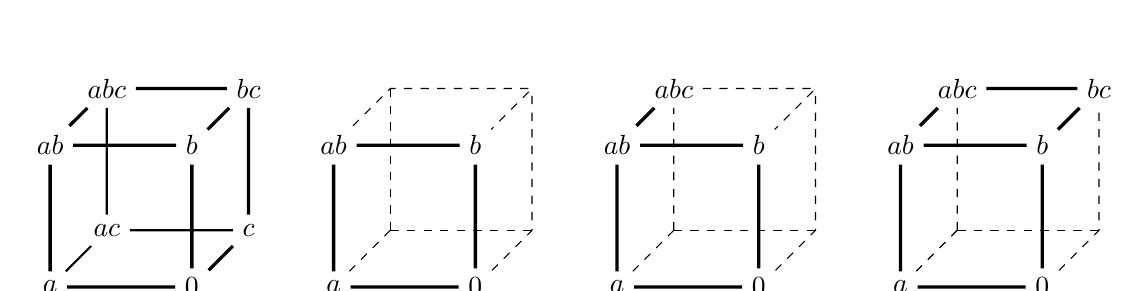
\begin{tikzpicture}[scale=1.8]
\begin{scope}[shift={(0,0)},local bounding box=aa]
    \node (0) at (0, 0) {$0$};
    \node (A) at (-1, 0) {$a$};
    \node (AB) at (-1, 1) {$ab$};
    \node (B) at (0, 1) {$b$};
    \node (C) at (0.4, 0.4) {$c$};
    \node (ABC) at (-0.6, 1.4) {$abc$};
    \node (BC) at (0.4, 1.4) {$bc$};
    \node (AC) at (-0.6, 0.4) {$ac$};

    \draw[very thick] (0) -- (A) -- (AB) -- (B) -- (0) ;
    \draw[very thick] (AB) -- (ABC) -- (BC) -- (B);
    \draw[very thick] (0) -- (C) -- (BC);

    \draw[thick] (AC) -- (A);
    \draw[thick] (AC) -- (ABC);
    \draw[thick] (AC) -- (C);        
\end{scope}

\begin{scope}[shift={(2,0)},local bounding box=bb]
    \node (0) at (0, 0) {$0$};
    \node (A) at (-1, 0) {$a$};
    \node (AB) at (-1, 1) {$ab$};
    \node (B) at (0, 1) {$b$};
    \coordinate (C) at (0.4, 0.4) {}; %{$c$};
    \coordinate (ABC) at (-0.6, 1.4) {}; % {$abc$};
    \coordinate (BC) at (0.4, 1.4) {}; % {$bc$};
    \coordinate (AC) at (-0.6, 0.4) {}; % {$ac$};

    \draw[very thick] (0) -- (A) -- (AB) -- (B) -- (0) ;
    \draw[dashed] (AB) -- (ABC) -- (BC) -- (B);
    \draw[dashed] (0) -- (C) -- (BC);

    \draw[dashed] (AC) -- (A);
    \draw[dashed] (AC) -- (ABC);
    \draw[dashed] (AC) -- (C);        
\end{scope}

\begin{scope}[shift={(4,0)},local bounding box=cc]
    \node (0) at (0, 0) {$0$};
    \node (A) at (-1, 0) {$a$};
    \node (AB) at (-1, 1) {$ab$};
    \node (B) at (0, 1) {$b$};
    \coordinate (C) at (0.4, 0.4) {};% {$c$};%
    \node (ABC) at (-0.6, 1.4) {$abc$};
    \coordinate (BC) at (0.4, 1.4) {};% {$bc$};%
    \coordinate (AC) at (-0.6, 0.4) {};% {$ac$};%

    \draw[very thick] (0) -- (A) -- (AB) -- (B) -- (0) ;
    \draw[very thick] (AB) -- (ABC);
    \draw[dashed] (ABC) -- (BC) -- (B);
    \draw[dashed] (0) -- (C) -- (BC);

    \draw[dashed] (AC) -- (A);
    \draw[dashed] (AC) -- (ABC);
    \draw[dashed] (AC) -- (C);        
\end{scope}

\begin{scope}[shift={(6,0)},local bounding box=dd]
    \node (0) at (0, 0) {$0$};
    \node (A) at (-1, 0) {$a$};
    \node (AB) at (-1, 1) {$ab$};
    \node (B) at (0, 1) {$b$};
    \coordinate (C) at (0.4, 0.4) {};% {$c$};%
    \node (ABC) at (-0.6, 1.4) {$abc$};
    \node (BC) at (0.4, 1.4) {$bc$};
    \coordinate (AC) at (-0.6, 0.4) {};% {$ac$};%

    \draw[very thick] (0) -- (A) -- (AB) -- (B) -- (0) ;
    \draw[very thick] (AB) -- (ABC) -- (BC) -- (B);
    \draw[dashed] (0) -- (C) -- (BC);

    \draw[dashed] (AC) -- (A);
    \draw[dashed] (AC) -- (ABC);
    \draw[dashed] (AC) -- (C);        
\end{scope}
\end{tikzpicture}
\caption{The Boolean lattice on 8 elements represented as a cube, and the 3 Heyting algebras of Figure \ref{fig:3HeytingAlgebras} embedded in this cube.}\label{fig:HAlgsInCubes}
\end{figure}

This hypercube representation immediately tells us that the Hasse diagrams of finite Heyting algebras are made up of lines and squares, and that no two squares can share more than one edge.  Figure \ref{fig:MoreHeytingAlgebras} illustrates a few more proper Heyting algebras, to give a sense of the range of shapes they can take.

\begin{figure}[htbp]
\centering
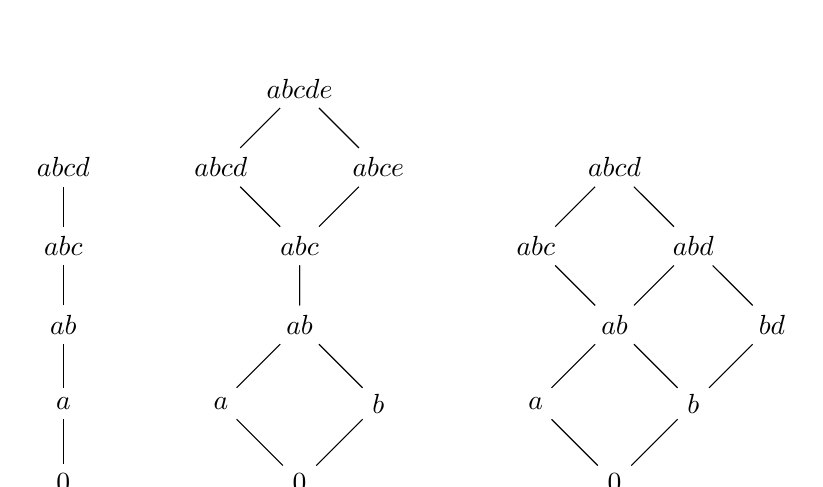
\begin{tikzpicture}[scale=.5]
\begin{scope}[shift={(0,0)},local bounding box=aa]
  \node (ABCD) at (0,8) {$abcd$};
  \node (ABC) at (0,6) {$abc$};
  \node (AB) at (0,4) {$ab$};
  \node (A) at (0,2) {$a$};
  \node (0) at (0,0) {$0$};
  
  \draw (0) -- (A)  -- (AB) -- (ABC) -- (ABCD); 
\end{scope}

\begin{scope}[shift={(6,0)},local bounding box=bb]
  \node (ABCDE) at (0,10) {$abcde$};
  \node (ABCD) at (-2,8) {$abcd$};
  \node (ABCE) at (2,8) {$abce$};
  \node (ABC) at (0,6) {$abc$};

  \node (AB) at (0,4) {$ab$};
  \node (A) at (-2,2) {$a$};
  \node (B) at (2,2) {$b$};
  \node (0) at (0,0) {$0$};
  
  \draw (0) -- (A)  -- (AB) -- (ABC) -- (ABCD) -- (ABCDE); 
  \draw (0) -- (B) -- (AB) -- (ABC) -- (ABCE) -- (ABCDE);
\end{scope}

\begin{scope}[shift={(14,0)},local bounding box=cc]
  \node (ABCD) at (0,8) {$abcd$};
  \node (ABC) at (-2,6) {$abc$};
  \node (ABD) at (2,6) {$abd$};
%  \node (AC) at (-4,4) {$ac$};
  \node (AB) at (0,4) {$ab$};
  \node (BD) at (4,4) {$bd$};
  \node (A) at (-2,2) {$a$};
  \node (B) at (2,2) {$b$};
  \node (0) at (0,0) {$0$};
  
  \draw (0) -- (A)  -- (AB) -- (ABC) -- (ABCD); 
  \draw (0) -- (B) -- (AB) -- (ABD) -- (ABCD);
%  \draw (A) -- (AC) -- (ABC);
  \draw (B) -- (BD) -- (ABD);
  \end{scope}



\end{tikzpicture}
\caption{Some more Heyting algebras.  Every chain forms a Heyting algebra (in which $\NOT x = 0$ for every element).  Heyting algebras can contain single edges between squares, as well as at the top and bottom.  Heyting algebras can be asymmetric.}\label{fig:MoreHeytingAlgebras}
\end{figure}



%\begin{table}[h]
%\centering
%\begin{tabular}{c|ccccc}
%$\IMPLIES$	& T & 2 & 3 & 4 & 0\\
%\hline
%T	&	T & 2 & 3 & 4 & 0	\\
%2	&	T & T & 3 & T & 3	\\
%3	&	T & 2 & T & T & 2	\\
%4	&	T & 2 & 3 & T & 0	\\
%0	&	T & T & T & T & T	\\
%\end{tabular}
%%
%\quad
%%
%\begin{tabular}{c|ccccc}
%$\AND$	& T & 2 & 3 & 4 & 0\\
%\hline
%T	&	T & 2 & 3 & 4 & 0	\\
%2	&	2 & 2 & 0 & 2 & 0	\\
%3	&	3 & 0 & 3 & 3 & 0	\\
%4	&	4 & 2 & 3 & 4 & 0	\\
%0	&	0 & 0 & 0 & 0 & 0	\\
%\end{tabular}
%%
%\quad
%%
%\begin{tabular}{c|ccccc}
%$\OR$	& T & 2 & 3 & 4 & 0\\
%\hline
%T	&	T & T & T & T & T	\\
%2	&	T & 2 & 4 & 4 & 2	\\
%3	&	T & 4 & 3 & 4 & 3	\\
%4	&	T & 4 & 4 & 4 & 4	\\
%0	&	T & 2 & 3 & 3 & 0	\\
%\end{tabular}
%\end{table} 




\subsection{Heyting algebras from preorders}

Another way to specify a Heyting algebra, which will be important in a later section, is to derive it as the lattice of upward closed sets of a preorder.  Let's unpack these terms.

A \terminology{preorder} is a binary relation on a set that is both reflexive and transitive, but need not be symmetric or antisymmetric.  We usually write the relation as $\leq$.

A subset $S$ of a preorder $(W, \leq)$ is \terminology{upward closed} 
if $x \in S$ and $x \leq y$ implies $y \in S$.  That is, if $S$ contains $x$ then it also contains every element of $W$ ``above'' $x$ in the preordering.  We will call an upward closed sets \emph{upsets} for short.  We will write $\uparrow x$ for the set of elements above $x$, i.e. $\uparrow x \DefinedAs \setSuchThat{y}{x \leq y}$, and we will call this the \emph{principal upset on $x$}.  An arbitrary upset is then a union of principal upsets.\footnote{
Trivially, the upset $S$ is the union $\bigcup_{s \in S} \uparrow S$, but there may be a smaller subset of $S$ that also serves as a base in this way (and a finite upset will always have a proper subset that serves as base).
}

Since upsets of $W$ are subsets of $W$, we can order them by subset inclusion.  We will now prove that this ordering on upsets makes then into a Heyting algebra.

\begin{Theorem}
The set of upsets on any preorder $(W, \leq)$, ordered by inclusion, form a Heyting algebra.
\end{Theorem}
\begin{Proof}
Let $(W, \leq)$ be a preorder.  We need to prove that the upsets of $(W, \leq)$ are closed under intersection and union, thus forming a lattice; that this lattice is bounded; and that we can define the $\to$ operation on lattice elements.  %
\begin{enumerate}[(a)]
\item If $P$ and $Q$ are upsets then for any element $i \in W$, 
\[
i \in P \intersect Q 
\iff
i \in P \mbox{ and } i \in Q
\]
Thus for any $j \geq i$, we have $j \in P$ and $i \in Q$, since $P$ and $Q$ are upsets, and thus $j \in P \intersect Q$.  Thus $P \intersect Q$ is also an upset.

\item If $P$ and $Q$ are upsets then for any element $i \in W$, 
\[
i \in P \union Q 
\iff
i \in P \mbox{ or } i \in Q
\]
Thus for any $j \geq i$, we either have $j \in P$ or $i \in Q$, since $P$ and $Q$ are upsets; in either case, $j \in P \union Q$.  Thus $P \union Q$ is also an upset.

\item The whole set $W$ itself is upward closed, and contains every upset as a subset; thus $W$ is the maximal element in the lattice.

\item The empty set $\varnothing$ is (trivially) upward closed, and is contained in every upset as a subset; thus $\varnothing$ is the minimal element in the lattice.

\item For upsets $P$ and $Q$, let 
\[
P \to Q
\DefinedAs
\setSuchThat{i \in W}{\uparrow i \subseteq \bar{P} \union Q}
\]
where $\bar{P} = W\setminus P$.  We will now prove that this satisfies the definition of $\to$ for a Heyting algebra, i.e. that it is the maximal upset $S$ such that $P \intersect S \subseteq Q$.
\begin{enumerate}[(i)]
\item First, $P \to Q$ is an upset: if 
$i \in P \to Q$ then $\uparrow i \subseteq \bar{P} \union Q$, and so for any $j \geq i$ we have ${\uparrow j} \subseteq {\uparrow i} \subseteq \bar{P} \union Q$, and thus $j \in P \to Q$.
%
\item Next, we prove that $P \intersect (P \to Q) \subseteq Q$.  Let 
$i \in P \intersect (P \to Q)$, so 
$\uparrow i \subseteq \bar{P} \union Q$, and so
$i \in \bar{P} \union Q$ (since the preorder relation is reflexive).  Thus 
\[
i \in (\bar{P} \union Q) \intersect P
= (\bar{P} \intersect P) \union (Q \intersect P)
= (Q \intersect P)
\]
by distributivity and the definition of $\bar{P}$.  Thus any $i$ in $P \intersect (P \to Q)$ is also in $Q$.
%
\item Finally, we prove that $P \to Q$ is the maximal such upset.  Let $X$ be an upset satisfying $X \intersect P \subseteq Q$.  Then we need to prove $X \subseteq (P \to Q)$.  Since $X$ is an upset, for any $x \in X$ we have $\uparrow x \subseteq X$.  But 
\[
X \intersect P \subseteq Q 
\iff
X \intersect P \intersect \bar{Q} = \varnothing
\iff
X \subseteq \bar{P} \intersect Q
\]
and so for any $x \in X$, $\uparrow x \subseteq X \subseteq \bar{P} \intersect Q$, and thus $x \in P \to Q$.
\end{enumerate}
\end{enumerate}
\end{Proof}

This gives us a useful way of constructing Heyting algebras -- we just give a preorder on some set and then order its upsets by subset inclusion.  As we'll see later, we can use this when we want to build Heyting algebra models of constructive logic satisfying certain properties.



\subsection{Logic with Heyting algebras}

Just as Boolean algebras provide the appropriate truth values for classical logic, Heyting algebras provide the appropriate truth values for constructive logic.


In Section \ref{sec:Models-TruthTables} we built a truth table for a formula in which each row corresponded to a way of assigning to each variable a truth value in the Boolean algebra $\{T, F\}$.  We can do exactly the same thing if we replace that Boolean algebra with any Heyting algebra -- since the usual logical operations are defined on a Heyting algebra, any assignment of values to the variables leads to a unique value for the formula itself.

We said that a formula is provable in CPL iff it is true under any assignment into $\{T, F\}$.  What is the corresponding result for constructive logic?  Which Heyting algebra plays the same role?  Unfortunately there is \emph{no} single Heyting algebra that serves the purpose.\footnote{As G\"{o}del proved in (1932).}  
However, what is true is that a formula is provable in constructive propositional logic iff it is a tautology -- i.e. gets the maximal value -- in \emph{every} Heyting algebra.  That means that if there is any assignment of values in any Heyting algebra that results in the formula getting a non-maximal value, then that formula is not provable constructively.  Thus we can still use truth tables to find  counterexamples to constructively invalid formulae.

As an example, consider again the formula 
$\NOT (P \AND Q) \IMPLIES ((\NOT P) \OR (\NOT Q))$.  We can evaluate this in any Heyting algebra, of course, but some will be more useful than others.  If we choose a Boolean algebra the formula will always get maximal value.  Likewise if we evaluate it in the 3-element chain.  But  in the 5-element Heyting algebra illustrated in Figure \ref{fig:3HeytingAlgebras} we can get a counterexample.  Since there are two variables we have $5^2=25$ rows to calculate, so we won't display the whole table -- but we don't need to.  To show that this formula is not constructively valid we just need to exhibit a single counterexample, i.e. a single row in which the formula does not have the maximal value $abc$ in that Heyting algebra, such as:
\begin{table}[h]
\centering
\begin{tabular}{c c|c c c}
P &	Q & $\NOT(P \AND Q)$ &	$(\NOT P) \OR (\NOT Q)$ &	$\NOT (P \AND Q) \IMPLIES ((\NOT P) \OR (\NOT Q))$ \\
\hline
a & b & 1 & ab & ab
\end{tabular}
\end{table}\\
That this is in fact a counterexample is easy to verify -- we simply have to evaluate the formula with the given values for the variables.  A Heyting algebra counterexample therefore provides a simple, compact, and easily verified demonstration that a given formula is not a tautology of constructive logic (and thus, via the Deduction theorem, that a given argument is not constructively valid).



\subsection{Building specific Heyting algebra counterexamples}

Although they are easy to verify, Heyting algebra counterexamples may not be easy to find.  For one thing, we do not know in advance \emph{which} Heyting algebra to evaluate into.  Then for any Heyting algebra we need to work out the entire truth table, which is a mechanical but tedious process.  It would be better, then, to have some means of producing counterexamples from formulae directly, or of demonstrating directly when a formula does not have a counterexample.

Ideally, what we would like (assuming we knew what Heyting algebra we should work in) is to construct a counterexample \emph{backwards}: starting with a non-maximal value in the right-most column of the truth table, we could then work from right to left, filling in the values that the preceding columns must take, until we eventually get to the left-most column containing the values of the variables.  


Of course, there are many factors that complicate matters.  First, we don't know which Heyting algebra we should be working in, and we don't yet even have a principle bounding the size of the Heyting algebras we need to consider.  Second, we don't know which non-maximal value the formula should take.  (For that matter, we don't even know in advance whether the formula has a counterexample at all -- that's what this process is supposed to find out.)  Then, for any given value in one column, there may be multiple compatible values that we could put in the preceding columns: for example, in two-valued Boolean logic, if we put $T$ in a column headed $A \OR B$ then there are 3 possible pairs of values we could assign to $A$ and $B$ that are compatible with this.  We would therefore need a \emph{branching} process, exploring each of these possibilities in parallel.

These various obstacles appear to make such a ``reverse-engineering'' of a counterexample unfeasible (or perhaps no less work than simply working out the whole truth table for a few Heyting algebras and hoping for some principle to guide us to the right one).  
However, a process based upon essentially this idea
 -- although with some major alterations! -- can be made to work, and this is the procedure we'll describe in the remainder of this section.

Rather than choosing the Heyting algebra in advance we will build it up indirectly by constructing a preorder by following certain rules depending upon the structure of the formula we are trying to disprove.  At the end of the procedure we will either have such a preorder, from which we can then obtain a Heyting algebra via the procedure of Section \ref{}, or we will find that no such preorder can be constructed.  In the latter case we wil have shown that there are no counterexamples to the formula, and thus the formula is a constructive tautology (and we should therefore direct our efforts into finding a constructive proof for it instead!)


\subsection{The rules of countermodel construction}

We want to define a preorder, so that we can obtain a Heyting algebra from it as its collection of upsets.  We also want to obtain an evaluation function from propositional variables and formulae into the Heyting algebra.  In particular, we want this evaluation to give a non-maximal value to the formula for which we are trying to give a countermodel.  So now we need to define a set of rules that will produce such a preorder for any formula that has a countermodel (i.e. any formula that is not a tautology of constructive logic).

If values in the Heyting algebra correspond to upsets in the preorder, then the valuation into the Heyting algebra, $h: F \to H$ should come from a valuation $\omega$ into the upsets of the preorder.  That is, for each formula $A$, $\omega(A)$ is an upward closed subset of the preorder.  It will also be useful to have a name for the complement of $\omega(A)$ in $W$, which we will denote $\bar{\omega}(A)$.


The valuation $h$ into the Heyting algebra that we obtain must be internally consistent -- for example, for any conjunction $A \AND B$ we must have $h(A \AND B) = h(A) \glb h(B)$.  If we pick values of $\omega$ arbitrarily then of course we can't expect this to hold, so we must impose rules on $\omega$ to guarantee consistency among values.  Specifically, we've seen in Section \ref{HAlgs-from-preorders} how the values must relate to one another: for all formulae $A$ and $B$,
\begin{itemize}
\item $\omega(A \AND B) \DefinedAs \omega(A) \intersect \omega{B}$
\item $\omega(A \OR B) \DefinedAs \omega(A) \union \omega{B}$
\item $\omega(A \to B) \DefinedAs 
\setSuchThat{i \in W}{\uparrow i \subseteq \bar{\omega}(A) \union \omega(B)}$
\end{itemize}
(where the latter condition follows from the fact that the upset corresponding to $A \to B$ must be the maximal upset $S$ such that $\omega(A) \intersect S \subseteq \omega(B)$.)

As usual, we define $\NOT A$ as $A \to \ABSURDITY$, where $\ABSURDITY$ is a contradictory proposition that is never true -- i.e. $\omega(\ABSURDITY) = \varnothing$.  Thus
\begin{itemize}
\item $\omega(\NOT A) \DefinedAs 
\setSuchThat{i \in W}{\uparrow i \subseteq \bar{\omega}(A)}$
\end{itemize}
Note that $\omega(\NOT A)$ is in general \emph{not} equal to $\bar{\omega}(A)$, but is always a subset of it.\footnote{
Proof sketch: if $i \in \omega(\NOT A)$ then $\uparrow i \subseteq \bar{\omega}(A)$, and we always have $i \in \uparrow i$, so 
$i \in \omega(\NOT A) \subseteq \bar{\omega}(A)$.  But for the converse dirction, $j \in \bar{\omega}(A)$ is not sufficient to guarantee $\uparrow j \subseteq \bar{\omega}(A)$, so in general $j \not\in \omega(\NOT A)$ and thus $\bar{\omega}(A) \not\subseteq \omega(\NOT A)$.
}
That is, $\omega(\NOT A) \intersect \omega(A) = \varnothing$, but 
$\omega(\NOT A) \union \omega(A) \neq W$, as we would expect for an intuitionistic logic.

We noted above that the whole preorder, being an upset, serves as the maximal element $1$ of the Heyting algebra.  Thus if the preorder has a root element -- i.e. a world $w_0$ such that $\forall w \in W,\, w_0 \leq w$ -- then any formula $A$ with $w_0 \in \omega(A)$ must (by the requirement that $\omega(A)$ be an upset) have $\omega(A) = W$, and therefore gets value $1$ in the Heyting algebra.  Conversely, to ensure that a formula $A$ does \emph{not} get maximal value in the Heyting algebra, we just need to ensure that $w_0 \not\in \omega(A)$.  This therefore gives our final two conditions when building a counterexample to $A$: ensure that the preorder has a root world $w_0$, and set $w_0 \not\in \omega(A)$.


So, given a formula $\phi$ that we wish to show is not a tautology, we  need to construct a rooted preorder $(W, \leq, w_0)$ and an evaluation function $\omega: F \to 2^W$ that assigns to each formula\footnote{
Specifically, to each formula using the same propositional variables as $\phi$.} 
an upward-closed subset of $W$, ensuring that $\omega$ obeys the rules above, and in which $w_0 \not\in \omega(\phi)$.  In the next section we will see the procedure that allows us to carry out this construction if it it possible.



%Another way to encode the same information is via a function $\nu: W \times F \to \set{0,1}$, defined by
%\[
%\nu(i, A) = 1 \quad \iff \quad i \in \omega(A)
%\]
%To ensure that the sets of worlds assigned to each formula are upward closed, we must impose a condition: if $\nu(i,A) = 1$ then for all $j \geq i$ in the preorder, $\nu(j,A) = 1$.

%For $\AND$ and $\OR$ the rules are obvious: for all $i \in W$, and all formulae $A$ and $B$,
%\[
%\nu(i,A \AND B) = 1 \quad \mbox{ iff } \quad 
%\nu(i,A) = 1 \mbox{ and } \nu(i,B) = 1
%\]
%\[
%\nu(i,A \OR B) = 1 \quad \mbox{ iff } \quad 
%\nu(i,A) = 1 \mbox{ or } \nu(i,B) = 1
%\]
%Equivalently, we can express these as sums and products of values:
%\begin{align*}
%\nu(i,A \AND B) &\DefinedAs 
%\nu(i,A) \times \nu(i,B)
%\\
%\nu(i,A \OR B) &\DefinedAs
%\nu(i,A) + \nu(i,B) - \nu(i,A) \times \nu(i,B)
%\end{align*}





%Part of the problem here is that when we do constructive logic all we know at a given time is which types we have terms for -- we have no way of positively recording the fact that we \emph{don't} have a term of a given type.  The mere omission of a term from the list of things we're given is not sufficient, since it may be possible to construct such a term from the things we are given and we have simply not yet done so.  That is, the fact that a term has not been constructed in a given context is not evidence that it \emph{cannot} be constructed in that context.  But it is precisely the latter that we need to demonstrate in order to show that a particular construction is not possible.  We therefore need a new approach to studying constructive arguments, in which both the presence and absence of terms can be actively recorded.
%
%In a constructive model, the failure to record that a term is present does not correspond to that term's being absent.  We models we require must therefore be \emph{classical}.  
%
%
%\subsubsection{Definition of Kripke models}
%
%A \terminology{Kripke frame} is a pair of a non-empty set $W$, whose elements we call \terminology{worlds}, and a binary relation $R$ on $W$, which we call \terminology{accessibility}.  For the most general Kripke frame we assume no particular properties of $R$.  However, for present purposes we will restrict attention to Kripke frames whose accessibility relations are \emph{reflexive} and \emph{transitive} (i.e. which are \emph{preorders}).  We therefore write the accessibility relation as $\leq$.
%
%An \terminology{intuitionistic Kripke model} is then a Kripke frame along with a relation $\makestrue$ between worlds and expressions of our language, such that:
%\begin{samepage}
%\begin{itemize}
%\item $w \makestrue A \AND B$ iff $w \makestrue A$ and $w \makestrue B$
%\item $w \makestrue A \OR B$  iff $w \makestrue A$ or  $w \makestrue B$
%\item $w \makestrue A \IMPLIES B$ iff for all $u \geq w$, $u \makestrue A$ implies $u \makestrue B$
%\item $w \not \makestrue \ABSURDITY$
%\item for any propositional variable, if $w \makestrue p$ and $w \leq u$ then $u \makestrue p$
%\end{itemize}
%\end{samepage}
%











%\newpage

%\setcounter{section}{6}
%\input{Section-RecursiveTypes}
%\newpage

% \setcounter{section}{9}	%% intended section number - 1
% \section{Quantifiers}
\label{sec:Quantifiers}

We have now demonstrated how a constructive propositional logic can be incorporated into our type theory.  But propositional logic isn't enough for the purposes of doing mathematics -- we need predicate logic as well.  We therefore need to find a way of incorporating \emph{quantifiers} as well.  In this section we'll see how to do that, first examining how the universal and existential quantifiers should be understood in constructive logic under the BHK interpretation, and then defining how they are implemented in the type theory.

Recall that in constructive logic under the BHK interpretation the meaning of a mathematical proposition is closely tied to its method of verification: we only say that a proposition is true when we have a witness to it, where witnesses to compound propositions are related to witnesses to their components.  Our first task, then, is to work out what a witness to a quantified proposition is.  


\subsection{Predicates and Universes}
\label{sec:Quantifiers-PredicatesUniverses}

A quantified proposition is of the form 
$(\forall x)\, \phi(x)$ or  
$(\exists x)\, \phi(x)$ 
for some \terminology{predicate} $\phi$, with $x$ ranging over some ``domain of discourse''.  Sometimes we make the domain of discourse explicit.  In set theory the domain of discourse will be a set $A$, so we would write 
$(\forall x \in A)\, \phi(x)$ or 
$(\exists x \in A)\, \phi(x)$.

\subsubsection{What is a predicate?}
\label{sec:Quantifiers-WhatIsAPredicate}

To translate this into our type theory we first need to translate the predicate $\phi$.  What is this?  $\phi$ itself is not a proposition -- it corresponds to something like ``\ldots~is red'' or ``\ldots is prime'', where the ``\ldots'' has not been filled in with any particular entity.\footnote{
Cite Frege on predicates as ``unsaturated'' functions.
}  
So it is more like a function that takes some entity $x$ as input and returns as output a proposition involving $x$.  For example, if $\phi$ corresponds to ``\ldots is prime'', then $\phi(5)$ is the proposition ``5 is prime'' and $\phi(12)$ is the proposition ``12 is prime''.

But what kind of function could this be?  A function of type $\type{A} \to \type{B}$ takes a terms of \type{A} as input and returns a term of \type{B}.  However, we want a predicate to be a function that takes a term of some type as input and returns a \emph{type} (i.e. a proposition) as output.  What could the type of such a function be?


\subsubsection{A new type called $\TYPE$}
\label{sec:Quantifiers-TypeCalledTYPE}

The answer to this, which might seem a little odd and perhaps a little dangerous at first, is to introduce a new type -- a type whose \emph{terms} are all the types we've encountered so far.
That is, for every type\footnote{
At least, every type that we've ben able to define so far -- see Section~\ref{} for a more precise statement.
}
\type{A}, 
\type{B}, 
$\type{X} \x \type{Y}$, etc. 
we have
$\type{A}:\TYPE$, 
$\type{B}:\TYPE$, 
$\type{X} \x \type{Y}:\TYPE$, etc. 

This solves our problem: 
a predicate \term{P} that asserts things about terms of type \type{A} is a function of type $\type{A} \to \TYPE$.  It takes a term $\term{x}:\type{A}$ as input, and returns $\type{P}(\term{x}):\TYPE$ as output.


Before we can accept this solution we need to overcome two difficulties: 
\begin{enumerate}
\item Doesn't introducing this ``type of types'' immediately open the door to paradox?  
\item This seems too weird -- isn't it incompatible with the whole idea of having terms and types as distinct things?
\end{enumerate}
Let's address the second issue first.

We first introduced types as ``kinds of things that a mathematical entity could be''.  
Some mathematical entities are integers, so \emph{integer} is a type; 
some mathematical entities are points in the Euclidean plane, so 
\emph{point in the Euclidean plane} is a type; and so on.  We didn't put any kind of limits on what types there are, so any well-defined ``kind of mathematical entity'' should correspond to a type.\footnote{
TODO: Update this to cover ``types as mathematical concepts''.
}

If we are to take this defining concept seriously, we have two options:
we can either \emph{deny} that types themselves are mathematical entities, in which case \emph{type} is not a kind of thing that mathematical entities could be; alternatively, if we accept that types are mathematical entities, we could deny the assumption that for every kind of mathematical entity there is a type to which they belong.
The former option seems unmotivated: we're doing mathematics and logic using types, so they certainly seem like mathematical entities of some kind.  The second option is somewhat less unmotivated, but needs to be spelled out in more detail.  Which kinds of mathematical entities don't have types that they belong to?  Is it just types themselves -- and if so, why?  The main motivation for making such a distinction likely boils down to worries about the potential for introducing paradox or circularity.  So let's deal with that issue now.



\subsubsection{Is \TYPE\ paradoxical?}
\label{sec:Quantifiers-IsTYPEParadoxical}

Introducing \TYPE\ seems dangerous because a type that contains all types as terms must contain itself as a term, which surely leads to trouble.  And indeed, if we had $\TYPE:\TYPE$ then a paradox would arise.\footnote{
TODO: Citation to Girard's paradox?
}
But this is \emph{not} what we're introducing here.	 Note that the proposal, as stated in Section~\ref{}, is to introduce ``a type whose terms are \emph{all the types we've encountered so far}''.  So the type \emph{integer} is a term of \TYPE, but \TYPE\ itself is not.  Likewise, nor is any predicate type $\type{A} \to \TYPE$, since these could not have been defined before we introduced \TYPE\ itself.  So, to be more precise, the terms of \TYPE\ are all the types whose definitions can be given without introducing \TYPE\ itself.

By making this small compromise we able to retain the idea that types are mathematical entities and every kind of mathematical entity belongs to a type -- without introducing paradox.

But wait!  Don't we have some exceptions to the above claim?  What about \TYPE, and $\type{A} \to \TYPE$, and any other types that we can now define involving \TYPE?  These all look like types, so shouldn't there be a type that they all belong to?  The answer of course is yes, and so we cannot rest at introducing just \TYPE\ alone.  To do justice to the idea that \emph{types are terms of some higher type} we must introduce a whole hierarchy $\TYPE_0$, $\TYPE_1$, $\TYPE_2$, \ldots, where what we've called \TYPE\ above is really $\TYPE_0$, and a type whose definition depends upon $\TYPE_i$ belongs to $\TYPE_{i+1}$.  To handle this hierarchy we invoke \terminology{Grothendieck universes}.\footnote{In the HoTT Book, $\TYPE_i$ is written $\mathcal{U}_i$.
}

However, this becomes a little complicated, and is not really necessary in order to understand the basic problem that we introduced \TYPE\ to solve: namely, the ability to define predicates.  So for now let's just use \TYPE, but use it carefully (in particular bearing in mind that \TYPE\ is something different from the types it contains -- we don't have $\TYPE:\TYPE$).  So \emph{strictly speaking} what we'll say in the following involving \TYPE\ is not quite correct since it ignores or collapses the hierarchy of universes, but be assured that it can be patched to be made rigorous when we eventually need to.

\newpage
\subsection{The BHK interpretation of quantifiers}
\label{sec:Quantifiers-BHKQuantifiers}

In this section we'll look at quantified statements in set theoretic notation, i.e. 
$(\forall x \in A)\, \phi(x)$ and 
$(\exists x \in A)\, \phi(x)$, and how to understand them under the BHK interpretation.  We'll work out how to translate them into type theory in the next section.

\subsubsection{BHK interpretation of universal quantifier}

Given a predicate $\phi$, the universally quantified proposition 
$(\forall x \in A)\, \phi(x)$
says of every element $x \in A$ that $\phi$ holds of it, i.e. that the proposition $\phi(x)$ is true.

As ever, under the BHK interpretation we can only assert that $\phi(x)$ is true when we have a witness to it, and so we can only claim that $\phi(x)$ is true for all $x \in A$
if we can produce a witness for each such proposition.  Thus, under the BHK interpretation, a witness to 
$(\forall x \in A)\, \phi(x)$
must be a function that maps elements $x \in A$ to witnesses to $\phi(x)$.




\subsubsection{BHK interpretation of existential quantifier}


Given a predicate $\phi$, the existentially quantified proposition 
$(\exists x \in A)\, \phi(x)$
says that there is at least one element $x \in A$ such that $\phi$ holds of it, i.e. such that the proposition $\phi(x)$ is true.

Again, we can only claim that $\phi(x)$ is true for a given $x$ if we have a witness to that proposition.  So we interpret the existentially qualified proposition as saying that there is at least one $x$ for which there is a witness to $\phi(x)$.  But again, it is not enough to claim that such an $x$ and such a witness exist -- we must be able to produce them.  Thus, under the BHK interpretation, a witness to 
$(\exists x \in A)\, \phi(x)$
consists of a particular $x \in A$, along with a witness to the proposition $\phi(x)$.



\subsection{Translating this into the type theory}
\label{sec:Quantifiers-TranslatingToTypeTheory}

We've seen how the quantified propositions are to be interpreted.  We've seen that a predicate $\phi$ corresponds to a function $\term{P}:\type{A} \to \TYPE$, 
which takes a term 
$\term{x}:\type{A}$ 
as input, 
and returns as output the type \type{P}(\term{x}) corresponding to the proposition $\phi(x)$.  For a given predicate $\term{P}:\type{A} \to \TYPE$ and a given $\term{x}:\type{A}$ we will often write terms of 
$\type{P}(\term{x})$ as 
$\term{p}^{\term{x}}:\type{P}(\term{x})$, 
where the superscript indicates which term of \type{A} they pertain to.


Now let's put this all together to see how to express quantified propositions in our type theory.




\subsubsection{Dependent Function Types}
\label{sec:Quantifiers-DependentFunctionTypes}

Corresponding to the universally quantified proposition 
$(\forall x \in A)\, \phi(x)$
there must be some type.  Its terms -- witnesses of the proposition -- must be functions that take
a term 
$\term{x}:\type{A}$ 
as input and return as output a term of type \type{P}(\term{x}).

This is unlike any function we have seen before, since all previous functions of some type $\type{A} \to \type{B}$ always returned outputs of a given \emph{fixed} type \type{B}.  The functions we require now give outputs whose type is different depending upon which \emph{term} of the input type they are given.  We therefore need to introduce new technology to our type theory -- a new way of forming types, alongside product, coproduct and function types -- called the \terminology{dependent function type}.  Since we write the dependent function type with the $\prod$ symbol, it is often referred to as the $\prod$-type.\footnote{
Alternatively it is also called the \terminology{dependent product type}, but we avoid this terminology.
}

The dependent function type 
has one type former, which takes a type \type{A} and a predicate on \type{A}, i.e. a function $\term{P}:\type{A} \to \TYPE$.  We write the resulting dependent function type as
\[
\PROD{\term{x}:\type{A}}{\type{P}(\term{x})}
\quad\quad\mbox{ or }\quad\quad
\AltPROD{\term{x}:\type{A}}{\type{P}(\term{x})}
\]
We use the former notation to emphasise the resemblance to universal quantification, and the latter to emphasise the resemblance to (non-dependent) functions.

There is one term constructor for the dependent function type, which is a straightforward generalisation of the $\lambda$-abstraction
we used for function types (see Section~\ref{}).  The only difference is that whereas 
$\lambda$-abstraction for function types
took an expression $\Phi$ of type \type{B} that involves a variable \term{x} of type \type{A}, 
for dependent function types we require an expression whose type \type{P}(\term{x}) depends upon \term{x}.  As before, we write the function as $\lambda \term{x} . \Phi$, or more clearly as $(\term{x} \mapsto \Phi)$.

Application of a dependent function is just the same as application of a non-dependent function: when we apply 
$\term{f}:\AltPROD{\term{x}:\type{A}}{\type{P}(\term{x})}$ 
to any $\term{x}:\type{A}$ 
we get some $\term{p}^{\term{x}}: \type{P}(\term{x})$.  

As a special case, for any given type \type{B} we can define the ``\emph{constant} predicate'' that assigns to each $\term{x}:\type{A}$ \emph{the same} type \type{B}.  (This corresponds to a degenerate predicate $\phi$ that just ignores its argument $x$ and returns the same proposition for any $x \in A$.)
When we choose a constant predicate for $\term{P}$ we get a ``dependent function type'', which we might write as 
$\term{f}:\AltPROD{\term{x}:\type{A}}{\type{B}}$, 
that is no longer dependent.  A term of this type is a function that, when applied to some $\term{x}:\type{A}$, returns some term $\term{f}(\term{x}):\type{B}$, i.e. it's just a function $\type{A} \to \type{B}$.  So (non-dependent) function types $\type{A} \to \type{B}$ are just special cases of dependent function types -- they're ones that have a ``constant predicate'' that picks the same type \type{B} for every term of its input.







\newpage
\subsubsection{Dependent Pair Types}
\label{sec:Quantifiers-DependentPairTypes}

Corresponding to the existentially quantified proposition 
$(\exists x \in A)\, \phi(x)$
there must be some type.  Its terms -- witnesses of the proposition -- must consist of pairs $(\term{x},\term{p}^{\term{x}})$, 
where
$\term{x}:\type{A}$ 
and 
$\term{p}^{\term{x}}:\type{P}(\term{x})$. 

This is unlike the pairs that are terms of the product type $\type{A}\x\type{B}$, since in that case the second component of every pair is of the given fixed type \type{B}.  The pairs we require now have second components whose type is different depending upon the first component.  We therefore need to introduce new technology to our type theory -- another new way of forming types -- called the \terminology{dependent pair type}.  Since we write the dependent pair type with the $\sum$ symbol, it is often referred to as the $\sum$-type.\footnote{
Alternatively it is also called the \terminology{dependent sum type}, but we will avoid this terminology.
}

The dependent pair type 
has one type former, which takes a type \type{A} and a predicate on \type{A}, i.e. a function $\term{P}:\type{A} \to \TYPE$.  We write the resulting dependent pair type as
\[
\SUM{\term{x}:\type{A}}{\type{P}(\term{x})}
\quad\quad\mbox{ or }\quad\quad
\AltSUM{\term{x}:\type{A}}{\type{P}(\term{x})}
\]
We use the former notation to emphasise the resemblance to existential quantification, and the latter to emphasise the resemblance to (non-dependent) products.

The term constructor for the 
dependent pair type 
is just like that of the product type, with the simple generalisation that when the first component is $\term{x}:\type{A}$, 
the type of the second component $\term{p}^{\term{x}}$ is \type{P}(\term{x}).


What about the elimination rule for dependent pairs?  Given an output type \type{Z}, how do we define a function 
of type 
$\left(\AltSUM{\term{x}:\type{A}}{\type{P}(\term{x})}\right) \to \type{Z}$?  In the non-dependent case, i.e. the product type, we could define a function $\term{f}:(\type{A} \x \type{B}) \to \type{Z}$ via a curried version
$\term{g}:\type{A} \to (\type{B} \to \type{Z})$, such that for each 
$\term{x}:\type{A}$ the output of
$\term{g}$ is a particular 
$\term{g}_{\term{x}}: \type{B} \to \type{Z}$.
Similarly, the curried version of a function out of a $\sum$-type
must be a function $\term{h}$ such that for each 
$\term{x}:\type{A}$ the output of
$\term{h}$ is a particular 
$\term{h}_{\term{x}}: \type{P}(\term{x}) \to \type{Z}$ whose input type depends upon $\term{x}$.  
%
%What is the type of this $\term{h}$?
%For each $\term{x}:\type{A}$ we need something depending upon $\term{x}$, so it must be a dependent function type.  The thing 
%$\term{h}_{\term{x}}$ 
%that we require for a given $\term{x}:\type{A}$ is of type $(\type{P}(\term{x}) \to \type{Z})$, so $\term{h}$ is of type
%$\AltPROD{\term{x}:\type{A}}{(\type{P}(\term{x}) \to \type{Z})}$.  
Given any dependent function of type 
$\AltPROD{\term{x}:\type{A}}{(\type{P}(\term{x}) \to \type{Z})}$ 
we can uncurry it to give a function of type
$\left(\AltSUM{\term{x}:\type{A}}{\type{P}(\term{x})}\right) \to \type{Z}$.


If, as in the previous section, we choose \term{P} to be a ``constant predicate'' that picks the same type \type{B} for each input $\term{a}:\term{A}$ then the resulting $\sum$-type, which we might write as
$\AltSUM{\term{a}:\type{A}}{\type{B}}$, is again no longer dependent.  The terms of this type will be pairs $(\term{a}, \term{b})$, i.e. terms of the product type $\type{A} \x \type{B}$.
So product types $\type{A} \x \type{B}$ are just special cases of dependent pair types -- they're ones that have a ``constant predicate'' that picks the same type \type{B} for every term of its input.









\subsection{Other uses of dependent types}
\label{sec:Quantifiers-OtherUsesDependentTypes}

Dependent function types have uses outside of their role as universally quantified propositions, which we'll see later.
But more interesting is the alternative interpretation we can give to $\sum$-types, aside from their role as existentially quantified propositions.

We noted above (Section~\ref{}) that there's a temptation to think of types and their terms as being like sets and their members.  While we should continue to resist this temptation, there are similarities (which we'll explore later in Section~\ref{}).
Just temporarily, let's set aside the admonition of Section~\ref{} and
take the analogy fairly literally.  On that understanding, the dependent pair type takes on a new interpretation.  If \type{A} is like a set of elements, then
$\AltSUM{\term{x}:\type{A}}{\type{P}(\term{x})}$
is (approximately) like the \emph{subset} of $\type{A}$ for which the property corresponding to $\type{P}$ holds, 
i.e. it's like 
$\setSuchThat{x \in A}{P(x)}$.  
%The first component of each pair in $\AltSUM{\term{x}:\type{A}}{\type{P}(\term{x})}$
%is a term of \type{A}, but (in general) not all the terms of \type{A} are included, only those terms \term{x} for which a witness to $\type{P}(\term{x})$ can be constructed.

However, it's not exactly what we would expect from a subset, because a term of
$\AltSUM{\term{x}:\type{A}}{\type{P}(\term{x})}$
consists of a pair 
$(\term{x}, \term{p}^{\term{x}})$, where 
$\term{x}:\type{A}$ and $\term{p}^{\term{x}}:\type{P}(\term{x})$.  
Another term of the type might be a pair
$(\term{y}, \term{q}^{\term{y}}_1)$ involving a
different 
$\term{y}:\type{A}$ 
along with a witness 
$\term{q}^{\term{y}}_1:\type{P}(\term{y})$.  
If $\type{P}(\term{y})$ has another term $\term{q}^{\term{y}}_2$ then 
the pair
$(\term{y}, \term{q}^{\term{y}}_2)$ is also a term of 
$\AltSUM{\term{x}:\type{A}}{\type{P}(\term{x})}$.
So the same term $\term{y}:\type{A}$ can occur multiple times in multiple pairs -- one for each distinct witness of $\type{P}(\term{y})$.  Counted this way, there might be \emph{many more} terms in $\AltSUM{\term{x}:\type{A}}{\type{P}(\term{x})}$
 than in \type{A} itself.  But let's set this issue aside for now.\footnote{
In  Section~\ref{} we'll see how to fix this.  Roughly speaking what we'll do is collapse all the distinct proofs for a given 
$\term{y}:\type{A}$ 
together, so we (effectively) have just a single pair $(\term{y}, \term{q}^{\term{y}})$ where originally we may have had multiple $(\term{y}, \term{q}^{\term{y}}_1)$, $(\term{y}, \term{q}^{\term{y}}_2)$, etc.
}

In these two interpretations of the dependent pair type we see an illustration of one of the biggest differences between constructive and classical logic.  In set theory built on FOL, the interpretation of $(\exists x \in A)\, \phi(x)$ and $\setSuchThat{x \in A}{\phi(x)}$ are completely different: the former is a proposition which is simply either true or false, while the latter is a set, an object that can have substantial content.  They're related, of course -- non-emptiness of the latter set is logically equivalent to the truth of the former proposition -- but conceptually they're quite disinct.

In our constructive logic, on the other hand, the distinction between the two notions is completely obscured.  Propositions are only asserted to be true when we construct witnesses to their truth, and so the proof of an \emph{existential} claim is an \emph{example}.  
Thus, since each example is as good a witness as any other, the idea of ``the collection of all...'' 
and the idea of 
``there exists some...'' 
collapse together.



\newpage




\subsection{Predicates and Relations}

Having defined predicates as things that assert propositions about the terms of some type, we should look at \emph{relations}, i.e. things that assert propositions about \emph{multiple} terms of \emph{multiple} types.  Just as a predicate on \type{A} is a function of type 
$\type{A} \to \TYPE$, so a relation is a function from multiple inputs to $\TYPE$.  

As with any function of multiple inputs, we can write it either as taking a single input of product type, e.g. 
$(\type{A} \x \type{B}) \to \TYPE$, or we can use currying to write it as $\type{A} \to (\type{B} \to \TYPE)$.  The latter will usually be more convenient for us, since it allows partial application: applying a relation of type
$\type{A} \to (\type{B} \to \TYPE)$ to a term $\term{a}:\type{A}$ gives a predicate 
of type $\type{B} \to \TYPE$ on \type{B}.\footnote{
This is just parallel to the familiar fact from set-based mathematics that from any relation $R \subseteq A \times B$ we can obtain the predicate $R(a,\cdot)$ on $B$.
}

The application of relation $\type{R}$ to inputs $\term{a}:\type{A}$ and $\term{b}:\type{B}$ therefore gives a type, whose terms are witnesses to the fact that $\term{x}$ and \term{y} stand in this relation.  We may write these terms as $\term{r}^{\term{x}\term{y}}:\type{R}(\term{a}, \term{b})$.\footnote{
Strictly, the type should be written 
$\type{R}(\term{a})(\term{b})$, or as $\type{R}((\term{a}, \term{b}))$ if we think of the relation as a predicate on a product type.  However, for simplicity we will simply write $\type{R}(\term{a}, \term{b})$.
}



Given a predicate $\type{R}$
%: (\type{A} \x \type{B}) \to \TYPE
we can of course form dependent function types and dependent pair types.  A dependent function using relation
$\type{R}$
will be of the form
\[
\AltPROD{\term{a}:\type{A}}{
(\AltPROD{\term{b}:\type{B}}
{\type{R}(\term{a},\term{b})})
}
\]
That is, it will be a function taking an $\term{a}$ and a $\term{b})$ as input and returning as output a term of $\type{R}(\term{a},\term{b})$.  
Thus a term of this dependent function type represents the universally quantified proposition 
$(\forall \term{a}:\type{A})(\forall \term{b}:\type{B}), {\type{R}(\term{a},\term{b})}$.

Similarly, the dependent pair type using relation $\type{R}$ may be written as
\[
\AltSUM{\term{a}:\type{A}}{
(\AltSUM{\term{b}:\type{B}}
{\type{R}(\term{a},\term{b})})
}
\]
and expresses the proposition
$(\exists \term{a}:\type{A})(\exists \term{b}:\type{B}), {\type{R}(\term{a},\term{b})}$.

We can of course define relations not just on product types but on dependent pair types as well.  Such a relation, which is a predicate of the form 
$\AltSUM



%We can generalise this to predicates on multiple arguments, to get things like
%$\PROD{\term{x}:\type{A}}
%{\PROD{\term{y}:\type{A}}
%{\term{Q}(\term{x},\term{y})}
%}$, where \term{Q} is now a function 
%$\term{Q}: \type{A} \to (\type{A} \to \TYPE)$.  
%
%\terminology{Reflexive} relations are those for which
%${\term{Q}(\term{x},\term{x})}$ 
%holds for all $\term{x}:\type{A}$.

%We can of course extend this to relations on more than two inputs by defining predicates on products of more than two types.


\subsection{Mixed quantification}


The above expressions involve just a single type of quantifier, either universal or existential.  However, we also want to be able to express mixed-quantifier propositions of the form 
\[
\forall \term{a}:\type{A},\, \exists \term{b}:\type{B},\, {\type{R}(\term{a},\term{b})}
\quad\quad
\mbox{and}
\quad\quad
\exists \term{a}:\type{A},\, \forall \term{b}:\type{B},\, {\type{R}(\term{a},\term{b})}
\]
We can do this very easily with dependent function and product types, as
\[
\PROD{\term{a}:\type{A}}{
\SUM{\term{b}:\type{B}}
{\type{R}(\term{a},\term{b})}}
\quad\quad
\mbox{and}
\quad\quad
\SUM{\term{a}:\type{A}}{
\PROD{\term{b}:\type{B}}
{\type{R}(\term{a},\term{b})}}
\]
respectively.  To unpack these we simply follow the definitions of the $\Pi$- and $\Sigma$-types involved:
\begin{itemize}
\item A term of 
$\PROD{\term{a}:\type{A}}{
\SUM{\term{b}:\type{B}}
{\type{R}(\term{a},\term{b})}}$
is a function that takes an $\term{x}:\type{A}$ as input and returns a pair $(\term{y}, \term{r}^{\term{x}\term{y}})$, where $\term{y}:\type{B}$ and 
$\term{r}^{\term{x}\term{y}}: 
\type{R}(\term{x},\term{y})$
\item A term of 
$\SUM{\term{a}:\type{A}}{
\PROD{\term{b}:\type{B}}
{\type{R}(\term{a},\term{b})}}$
is a pair $(\term{x},\term{f})$ where $\term{x}:\type{A}$ and
$\term{f}:
\PROD{\term{b}:\type{B}}
{\type{R}(\term{x},\term{b})}$ is a function that takes a $\term{y}:\type{B}$ and returns a $\term{r}^{\term{x}\term{y}}: 
\type{R}(\term{x},\term{y})$.
\end{itemize}
We can of course extend this to produce propositions with any number of quantifiers.



\newpage
\subsection{Quantifying over other types}

We have seen that quantifying over a product type $\type{A} \x \type{B}$ is equivalent to quantifying separately over each of the two types \type{A} and \type{B}.  What about other types?

\subsubsection{Quantifying over coproducts}

A term of 
$\PROD{\term{c}:\type{A} \+ \type{B}}{\type{R}(\term{c})}$
says that $\type{R}$ holds for any term of \type{A}, and for any term of \type{B}.  Thus this should be equivalent to 
$\PROD{\term{a}:\type{A}}{\type{R}(\term{a})} \x
\PROD{\term{b}:\type{B}}{\type{R}(\term{b})}$.

A term of 
$\SUM{\term{c}:\type{A} \+ \type{B}}{\type{R}(\term{c})}$
says that $\type{R}$ holds for some term that is either a term of \type{A} or a term of \type{B}.  Thus this should be equivalent to 
$\SUM{\term{a}:\type{A}}{\type{R}(\term{a})} \+
\SUM{\term{b}:\type{B}}{\type{R}(\term{b})}$.

Of course, the above cannot be quite right as stated, since in each case \type{R} is a predicate with a particular input type, and so we cannot simply change its input type from $\type{A} \+ \type{B}$ to \type{A}.  We therefore need to be more careful about our definitions.

% \newpage

%\setcounter{section}{10}	%% intended section number - 1
%\section{Predicate Logic in Type Theory}
\label{sec:PredicateLogic}

Now we've introduced the quantifiers into our language we need to investigate how they behave.  How much of classical (first order) \terminology{predicate logic} is preserved when we work in this constructive system?\footnote{
Question: To what extent can we get quantified formulae into prenex normal form (i.e. with all quantifiers at the front?  We can't move negations inside, but what about $\AND$, $\OR$, and $\IMPLIES$?
%http://en.wikipedia.org/wiki/Prenex_normal_form
}
(Note that, as in Section~\ref{}, we're (currently) working in a \emph{semantic} rather than \emph{syntactic} style, i.e. we're thinking about manipulating and constructing terms rather than simply applying purely formal introduction and elimination rules to expressions.)


\subsection{Quantifiers and Conjunction or Disjunction}
\label{sec:PredicateLogic-QuantifiersANDOR}

Given two predicates $\term{P}$ and $\term{Q}$ on the type $\type{A}$, we can define a number of propositions involving a single quantifier and either a conjunction or a disjunction.  How do they relate to one another?  We will see that in all the following cases, the rule holds constructively exactly when it holds classically.  (For the cases where the rule does not hold, it is easy to get a counterexample: consider the case where we quantify over the natural numbers, and $\term{P}(\term{n})$ is ``$\term{n}$ is even'' while $\term{Q}(\term{n})$ is ``$\term{n}$ is odd''.)


\subsubsection{Universal quantifier and conjunction}

\[
(\forall x \in A) (P(x) \AND Q(x))
	\;\; \dashv \; \tstile \;\;
((\forall y \in A) P(y)) \AND ((\forall z \in A) Q(z))
\]
\[
\PROD{\term{x}:\type{A}}
{(
\type{P}(\term{x})
\x
\type{Q}(\term{x})
)}
	\;\; \dashv \; \tstile \;\;
\left(
\PROD{\term{y}:\type{A}}
{\type{P}(\term{y})}
\right)
\x
\left(
\PROD{\term{z}:\type{A}}
{\type{Q}(\term{z})}
\right)
\]

A term $\term{f}:\PROD{\term{x}:\type{A}}
{(
\type{P}(\term{x})
\x
\type{Q}(\term{x})
)}$
is a function that takes $\term{x}:\type{A}$ as input and returns as output a term of 
$(\type{P}(\term{x})
\x
\type{Q}(\term{x}))$, i.e. a pair 
$(\term{p}^{\term{x}},
\term{q}^{\term{x}})$.

A term $(\term{g}, \term{h}):
\left(
\PROD{\term{y}:\type{A}}
{\type{P}(\term{y})}
\right)
\x
\left(
\PROD{\term{z}:\type{A}}
{\type{Q}(\term{z})}
\right)$
is a pair of functions, where 
$\term{g}: \PROD{\term{y}:\type{A}}
{\type{P}(\term{y})}$
takes a term $\term{y}:\type{A}$ as input and returns a term 
$\term{p}^{\term{y}}: \type{P}(\term{y})$, while 
$\term{h}: \PROD{\term{z}:\type{A}}
{\type{Q}(\term{z})}$
takes a term $\term{z}:\type{A}$ as input and returns a term 
$\term{q}^{\term{z}}:\type{Q}(\term{z})$.


$\tstile$: Given \term{f} we use the projectors $pr_1$ and $pr_2$ from the product, and define 
$\term{g}(\term{x}) \DefinedAs pr_1(\term{f}(\term{x}))$ and 
$\term{h}(\term{x}) \DefinedAs pr_2(\term{f}(\term{x}))$.

$\dashv$: Given $(\term{g}, \term{h})$ we define
$\term{f}(\term{x}) \DefinedAs 
(\term{g}(\term{x}), \term{h}(\term{x}))$.


\newpage
\subsubsection{Existential quantifier and conjunction}

\[
(\exists x \in A) (P(x) \AND Q(x))
	\;\; \not\dashv \; \tstile \;\;
((\exists y \in A) P(y)) \AND ((\exists z \in A) Q(z))
\]
\[
\SUM{\term{x}:\type{A}}
{(
\type{P}(\term{x})
\x
\type{Q}(\term{x})
)}
	\;\; \not\dashv \; \tstile \;\;
\left(
\SUM{\term{y}:\type{A}}
{\type{P}(\term{y})}
\right)
\x
\left(
\SUM{\term{z}:\type{A}}
{\type{Q}(\term{z})}
\right)
\]

A term of 
$\SUM{\term{x}:\type{A}}
{(
\type{P}(\term{x})
\x
\type{Q}(\term{x})
)}$
is a pair 
$(\term{x}, (\term{p}^{\term{x}}, \term{q}^{\term{x}}))$, where $\term{x}:\type{A}$, $\term{p}^{\term{x}}:\type{P}(\term{x})$, and $\term{q}^{\term{x}}:\type{Q}(\term{x})$.

A term of 
$%\left(
\SUM{\term{y}:\type{A}}
{\type{P}(\term{y})}
%\right)
\x
%\left(
\SUM{\term{z}:\type{A}}
{\type{Q}(\term{z})}
%\right)
$
is a pair 
$((\term{y},\term{p}^{\term{y}}), (\term{z},\term{q}^{\term{z}}))$,
% 
where $\term{y}:\type{A}$, $\term{z}:\type{A}$, $\term{p}^{\term{y}}:\type{P}(\term{y})$, and $\term{q}^{\term{z}}:\type{Q}(\term{z})$.  NB: Note that we won't in general have the \emph{same} term of $\type{A}$ involved in both components of this pair, so must give them different names -- but nothing \emph{forces} the terms to be different, so we also have the case where the same term appears on both sides (i.e. where $\term{y} \equiv \term{z}$).


$\tstile$: Given $(\term{x}, (\term{p}^{\term{x}}, \term{q}^{\term{x}}))$ we can immediately construct 
$((\term{x},\term{p}^{\term{x}}), (\term{x},\term{q}^{\term{x}}))$, which is a term of 
$\left(
\SUM{\term{a}:\type{A}}
{\type{P}(\term{a})}
\right)
\x
\left(
\SUM{\term{a}:\type{A}}
{\type{Q}(\term{a})}
\right)$.


$\not\dashv$:  This is not constructively valid, as we'd expect, since in general we don't have $\term{y} \equiv \term{z}$ in the pair of terms provided.  








\subsubsection{Universal quantifier and disjunction}

\[
(\forall x \in A) (P(x) \OR Q(x))
	\;\; \dashv \; \not\tstile \;\;
((\forall y \in A) P(y)) \OR ((\forall z \in A) Q(z))
\]
\[
\PROD{\term{x}:\type{A}}
{(
\type{P}(\term{x})
\+
\type{Q}(\term{x})
)}
	\;\; \dashv \; \not\tstile \;\;
\left(
\PROD{\term{y}:\type{A}}
{\type{P}(\term{y})}
\right)
\+
\left(
\PROD{\term{z}:\type{A}}
{\type{Q}(\term{z})}
\right)
\]

A term 
$\term{f}:\PROD{\term{x}:\type{A}}
{(
\type{P}(\term{x})
\+
\type{Q}(\term{x})
)}$ 
is a function that takes $\term{x}:\type{A}$ as input and returns as output a term of 
$\type{P}(\term{x})
\+
\type{Q}(\term{x})$, i.e. either a term 
$\term{p}^{\term{x}}:\type{P}(\term{x})$
or a term
$\term{q}^{\term{x}}:\type{Q}(\term{x})$.


A term of
$%\left(
\PROD{\term{y}:\type{A}}
{\type{P}(\term{y})}
%\right)
\+
%\left(
\PROD{\term{z}:\type{A}}
{\type{Q}(\term{z})}
%\right)
$ 
is either a function 
$\term{g}:
%\left(
\PROD{\term{y}:\type{A}}
{\type{P}(\term{y})}
%\right)
$
or a function
$\term{h}:
%\left(
\PROD{\term{z}:\type{A}}
{\type{Q}(\term{z})}
%\right)
$.

$\not\tstile$:  This is not constructively valid, as we would expect -- in general we cannot guarantee that \term{f} will output a 
$\term{p}^{\term{x}}:\type{P}(\term{x})$ for every $\term{x}:\type{A}$, nor that it will output a 
$\term{q}^{\term{x}}:\type{Q}(\term{x})$ for every $\term{x}:\type{A}$, and so we cannot construct either of \term{g} or \term{h}.



$\dashv$:  Trivially, by case analysis on the coproduct: 
if we have \term{g} then we define $\term{f}(\term{a}) \DefinedAs 
\term{g}(\term{a})$, whereas 
if we have \term{h} then we define $\term{f}(\term{a}) \DefinedAs 
\term{h}(\term{a})$.



\newpage
\subsubsection{Existential quantifier and disjunction}

\[
(\exists x \in A) (P(x) \OR Q(x))
	\;\; \dashv \; \tstile \;\;
((\exists y \in A) P(y)) \OR ((\exists z \in A) Q(z))
\]
\[
\SUM{\term{x}:\type{A}}
{(
\type{P}(\term{x})
\+
\type{Q}(\term{x})
)}
	\;\; \dashv \; \tstile \;\;
\left(
\SUM{\term{y}:\type{A}}
{\type{P}(\term{y})}
\right)
\+
\left(
\SUM{\term{z}:\type{A}}
{\type{Q}(\term{z})}
\right)
\]

A term of 
$\SUM{\term{x}:\type{A}}
{(
\type{P}(\term{x})
\+
\type{Q}(\term{x})
)}$
is a pair $(\term{x}, \term{g}^{\term{x}})$, where $\term{g}^{\term{x}}$ is either $inl(\term{p}^{\term{x}})$ for some
$\term{p}^{\term{x}}:\type{P}(\term{x})$ or
$inr(\term{q}^{\term{x}})$ for some
$\term{q}^{\term{x}}:\type{Q}(\term{x})$.


A term of 
$%\left(
\SUM{\term{y}:\type{A}}
{\type{P}(\term{y})}
%\right)
\+
%\left(
\SUM{\term{z}:\type{A}}
{\type{Q}(\term{z})}
%\right)
$
is either a pair 
$(\term{y},\term{p}^{\term{y}})$ with $\term{y}:\type{A}$, and $\term{p}^{\term{y}}:\type{P}(\term{y})$,
or a pair 
$(\term{z},\term{q}^{\term{z}})$ with $\term{z}:\type{A}$, and $\term{q}^{\term{z}}:\type{Q}(\term{z})$.

Both directions of this proof are trivial, requiring only that we unwrap coproduct terms through case analysis and then re-wrap things with the relevant coproduct injectors.  No further construction is required.




%\subsubsection{Summary and Generalisation}

%From the above facts and a couple of other results, it follows that the whole ``cube'' of classical entailments between statements of this kind also hold constructively.


\subsection{Quantifiers and Negation}
\label{sec:PredicateLogic-QuantifiersNegation}

Classically we can ``pull negations past quantifiers'', for example transforming $\NOT \forall$ into $\exists \NOT$ and vice versa.  Can we do that in our constructive logic?  There are four classical relationships to test.  Written in set-theoretic notation, they look like this:

\begin{table}[h]
\centering
\begin{tabular}{r c r }
$(\forall a \in A) P(x)$					&$\dashv \; \tstile$ 	
&$\NOT (\exists a \in A) \NOT P(x)$
 \\
$(\forall a \in A) \NOT P(x)$					&$\dashv \; \tstile$ 	
&$\NOT (\exists a \in A) P(x)$
 \\
$\NOT(\forall a \in A) P(x)$					&$\dashv \; \tstile$ 	
&$(\exists a \in A) \NOT P(x)$
 \\
$\NOT(\forall a \in A) \NOT P(x)$					&$\dashv \; \tstile$ 	
&$(\exists a \in A) P(x)$
\end{tabular}
\end{table}
(where $P$ is some arbitrary predicate on the set $A$).

Schematically, we could write these as:

\begin{table}[h]
\centering
\begin{tabular}{r c l}
$\forall$					&$\dashv \; \tstile$ 	
&$\NOT \exists\NOT $
 \\
$\forall\NOT $					&$\dashv \; \tstile$ 	
&$\NOT \exists$
 \\
$\NOT\forall$					&$\dashv \; \tstile$ 	
&$\exists\NOT $
 \\
$\NOT\forall\NOT $					&$\dashv \; \tstile$ 	
&$\exists$
\end{tabular}
\end{table}

As with the case of de Morgan's laws (Section~\ref{}), we'll find that some of these hold constructively and some don't.  We'll deal with the two middle rows of the table first, and use these results in proving results for the other two rows.




\subsubsection{$\forall\NOT$ and $\NOT \exists$}

\[
(\forall a \in A) \NOT P(a)
\;\; \dashv \; \tstile 	\;\; 
\NOT (\exists a \in A) P(a)
\]
\[
\term{f}:\PROD
{\term{a}:\type{A}}
{(\type{P(a)} \to \z)}
\;\; \dashv \; \tstile 	\;\; 
\term{g}:\left(
\SUM{\term{a}:\type{A}}{\type{P(a)}}
\right) \to \z
\]

$\tstile$:  We are given a term 
$\term{f}:\PROD
{\term{a}:\type{A}}
{(\type{P(a)} \to \z)}$, 
and we want to use this to construct a function 
$\term{g}: \left(
\SUM{\term{a}:\type{A}}{\type{P(a)}}
\right) \to \z$.  
The function $\term{g}$ must take any witness of 
$\SUM{\term{a}:\type{A}}{\type{P(a)}}$
and return a term of $\z$.  

A term of 
$\SUM{\term{a}:\type{A}}{\type{P(a)}}$, 
recall, is a pair $(\term{x}, \term{p}^{\term{x}})$ consisting of a term $\term{x}:\type{A}$ 
and a term $\term{p}^{\term{x}}:\type{P(x)}$.  So we can think of  $\term{g}$ as taking any purported witness and discrediting it (by showing that a term of $\z$ can be obtained from it).

To do this, we just have to apply $\term{f}$ to the given $\term{x}:\type{A}$, which will produce a corresponding 
$\bar{\term{p}}^{\term{x}}: \type{P(x)} \to \z$.  We can then apply this 
$\bar{\term{p}}^{\term{x}}$ to the provided $\term{p}^{\term{x}}$ to get the term of $\z$ we need.  So we can define $\term{g}$ as 
$\term{g}((\term{x}, \term{p}^{\term{x}})) \DefinedAs 
\term{f}(\term{x})(\term{p}^{\term{x}})$



$\dashv$: Given a function \term{g} that discredits purported witnesses $(\term{x},\term{p}^{\term{x}})$, can we build a function $\term{f}$ that returns a particular $\term{f}_{\term{x}}: \type{P(x)} \to \z$ for each $\term{x}:\type{A}$?  What must $\term{f}_{\term{x}}$ do when given a term $\term{p}^{\term{x}}:\type{P(x)}$, in order to produce a term of $\z$?  It can just feed that $\term{p}^{\term{x}}$, along with its own particular $\term{x}$, into $\term{g}$.  Thus we can define
$\term{f}(\term{x})(\term{p}^{\term{x}})
 \DefinedAs 
\term{g}((\term{x}, \term{p}^{\term{x}}))$.




\subsubsection{$\NOT\forall$ and $\exists \NOT$}

\[
\NOT(\forall a \in A) P(x)
\;\; \dashv \; \tstile 	\;\; 
(\exists a \in A) \NOT P(x)
\]
\[
\bar{\term{f}}:
\left(
\PROD
{\term{a}:\type{A}}
{\type{P(a)}}
\right) \to \z
\;\; \dashv \; \tstile 	\;\; 
(\term{x}, \bar{\term{p}}^{\term{x}}):
\SUM{\term{a}:\type{A}}
{(\type{P(a)} \to \z)}
\]

$\not\tstile$:  This is not constructively valid.  In order to produce the ``counterexample'' $(\term{x}, \bar{\term{p}}^{\term{x}})$ we need to produce a term $\term{x}:\type{A}$, but for arbitrary types we cannot in general produce a term.  Having the function $\bar{\term{f}}$ doesn't help.

In fact, if we consider the special case where, for all $\term{a}:\type{A}$, we define the type $\type{P(a)}$ to simply be the type $\z$ then we see that if we could carry out this construction we could obtain a term of \type{A} from a term of $(\type{A} \to \z) \to \z$ -- i.e. we could do DNE.

$\dashv$:  We are given a term
$(\term{x}, \bar{\term{p}}^{\term{x}}):
\SUM{\term{a}:\type{A}}
{(\type{P(a)} \to \z)}$, 
where $\term{x}:\type{A}$ and 
$\bar{\term{p}}^{\term{x}}:\type{P(x)} \to \z$, 
and we want to use it to construct a function 
$\bar{\term{f}}:
\left(
\PROD
{\term{a}:\type{A}}
{\type{P(a)}}
\right) \to \z$.  This function $\bar{\term{f}}$ 
must take functions 
$\term{f}:\PROD
{\term{a}:\type{A}}
{\type{P(a)}}$ 
and discredit them by showing that they can be used to obtain to a term of $\z$.

To do this, all we need is to apply \term{f} to our ``counterexample'' \term{x} to get 
$\term{f}(\term{x}):\type{P(x)}$.  Then the provided 
$\bar{\term{p}}^{\term{x}}$ can be applied to this to give the required term of $\z$.  Thus we can define 
$\bar{\term{f}}$ as
$\bar{\term{f}}(\term{f}) \DefinedAs 
\bar{\term{p}}^{\term{x}}(\term{f}(\term{x}))$








\subsubsection{$\forall$ and $\NOT \exists \NOT$}

\[
(\forall a \in A) P(x)
\;\; \dashv \; \tstile 	\;\; 
\NOT (\exists a \in A) \NOT P(x)
\]
\[
\term{f}:\PROD{\term{a}:\type{A}}{\type{P(a)}}
\;\; \dashv \; \tstile 	\;\; 
\term{g}:
\left(
\SUM{\term{a}:\type{A}}{(\type{P(a)} \to \z)}
\right) \to \z
\]

$\tstile$:  From 
$\term{f}:\PROD{\term{a}:\type{A}}{\type{P(a)}}$
we can construct
$\term{f}^{\prime}:\PROD{\term{a}:\type{A}}
{((\type{P(a)} \to \z) \to \z)}$
by DNI. Specifically, $\term{f}^{\prime}(\term{x})$ applies \term{f} to \term{x} to get a term of $\type{P(x)}$, and then applies the construction described in Section~\ref{} to produce a term of 
${(\type{P(x)} \to \z) \to \z}$.

$\PROD{\term{a}:\type{A}}
{((\type{P(a)} \to \z) \to \z)}$ corresponds to the proposition
$(\forall a \in A) \NOT \NOT P(x)$.  Using the construction of Section~\ref{} above we can therefore ``pull'' one of the negation signs past the quantifier.  That is, we can use this $\term{f}^{\prime}$ to construct a term of 
$\left(
\SUM{\term{a}:\type{A}}{(\type{P(a)} \to \z)}
\right) \to \z$
corresponding to the proposition
$\NOT(\exists a \in A) \NOT P(x)$, as required.




$\not\dashv$:  This is not constructively valid.
\term{g} takes any pair $(\term{x},\bar{\term{p}}^{\term{x}})$ and returns a term of $\z$.  But to construct \term{f} we need a way to map any given \term{a} to a corresponding term $\term{p}^{\term{a}}:\type{P(a)}$, and \term{g} is no help in doing this.

In particular, if we consider the special case where for every $\term{a}:\type{A}$ we choose $\type{P(a)}$ to be \type{B} (i.e. consider a non-dependent function $\type{A} \to \type{B}$) then we can show that this construction would allow us to carry out DNE.\footnote{
Specifically, if we ``quantify'' over the Unit type \type{1} that has exactly one term.  The details are left as an exercise.}

%Of course, we can use the result proved above to ``pull'' the first negation past the $\exists$ quantifier, thereby demonstrating 
%\[
%\NOT (\exists a \in A) \NOT P(x)
%\;\; \tstile 	\;\; 
%(\forall a \in A) \NOT \NOT P(x)
%\]
%but since we can't do DNE this does not give us 
%$(\forall a \in A) P(x)$.




\subsubsection{$\NOT\forall\NOT$ and $\exists$}

\[
\NOT(\forall a \in A) \NOT P(a)
\;\; \dashv \; \tstile 	\;\; 
(\exists a \in A) P(a)
\]
\[
\bar{\term{f}}:
\left(
\PROD{\term{a}:\type{A}}
{(\type{P(a)} \to \z)}
\right) \to \z
	\;\; \dashv \; \tstile 	\;\; 
(\term{x}, \term{p}^{\term{x}}):
\SUM{\term{a}:\type{A}}
{\type{P(a)}}
\]


$\not\tstile$: This is not constructively valid.  We need to construct a particular term $\term{x}:\type{A}$, but $\bar{\term{f}}$ doesn't provide anything to help us do this.

Moreover, if we could carry out this construction then we could use it to do DNE (by taking ${\type{P(a)}}$ to be a constant \type{B} for all $\term{a}:\type{A}$, and `quantifying' over the Unit type). 

$\dashv$:  $\bar{\term{f}}$ takes any function 
$\term{f}:\PROD{\term{a}:\type{A}}
{(\type{P(a)} \to \z)}$
and applies it to \term{x} to get some 
$\bar{\term{p}}^{\term{x}}:{\type{P(x)} \to \z}$.  This function can then be applied to $\term{p}^{\term{x}}:\type{P(x)}$ to get the required term of $\z$.  Thus we can define $\bar{\term{f}}$ as
$\bar{\term{f}}(\term{f}) \DefinedAs
\term{f}(\term{x})(\term{p}^{\term{x}})$.




\subsubsection{Summary}

So, just as in the case of the de Morgan laws, 5 of the 8 classical entailments are constructively valid, and 3 are not.  We can summarise the results in the following schematic table:

\begin{table}[h]
\centering
\begin{tabular}{r c l}
$\forall$					&$\not\dashv \; \tstile$ 	
&$\NOT \exists\NOT $
 \\
$\forall\NOT $					&$\dashv \; \tstile$ 	
&$\NOT \exists$
 \\
$\NOT\forall$					&$\dashv \; \not\tstile$ 	
&$\exists\NOT $
 \\
$\NOT\forall\NOT $					&$\dashv \; \not\tstile$ 	
&$\exists$
\end{tabular}
\end{table}

Moreover, if we compare these results with the corresponding table we got for de~Morgan's laws, we can see that they are in exact parallel:

\begin{table}[h]
\centering
\begin{tabular}{r c l || c c c}
$(A \AND B)$					
&$\not\dashv \; \tstile$ 	
&$\NOT(\NOT A \OR \NOT B)$
%
&$\forall$					
&$\not\dashv \; \tstile$ 	
&$\NOT \exists\NOT $
 \\  %%%%%%%%%%%%%%%%
$(\NOT A \AND \NOT B)$ 	 	
&$\dashv \; \tstile$ 	
&$\NOT(A \OR B)$ 
%
&$\forall\NOT $					
&$\dashv \; \tstile$ 	
&$\NOT \exists$
 \\  %%%%%%%%%%%%%%%%
$\NOT(A \AND B)$  				
&$\dashv \; \not\tstile$ 	
&$(\NOT A \OR \NOT B)$
%
& $\NOT\forall$					
&$\dashv \; \not\tstile$ 	
&$\exists\NOT $
 \\  %%%%%%%%%%%%%%%%
$\NOT (\NOT A \AND \NOT B)$	
&$\dashv \; \not\tstile$ 	
&$(A \OR B)$
%
& $\NOT\forall\NOT $					
&$\dashv \; \not\tstile$ 	
&$\exists$
\end{tabular}
\end{table}

This brings up a different connection between dependent and non-dependent types.  In Section~\ref{} we saw that dependent function types include as a special case the non-dependent function types, and dependent pair types include as a special case the product types.  The above correspondence, on the other hand, suggests that we might think of 
universal quantification as a generalised kind of conjunction, and 
existential quantification as a generalised kind of disjunction (which is already a familiar idea from classical logic).  

In fact, we can go further than this.  If we hadn't defined product and coproduct types, we could have defined them as special kinds of $\prod$- and $\sum$-types respectively, where the type quantified over has exactly two terms (see Section~\ref{} for the definition of this type).\footnote{However, some of the details of what we end up with by doing things this way end up being a bit different.  For more about this, see the HoTT Book, pp. 35--36.
}
%Drawing these facts together in a table:
%
%\begin{table}[h]
%\centering
%\begin{tabular}{c c c c}
%Non-dependent	&	Dependent	&	Quantifier	&	\ldots which generalises 
%\\
%\hline
%$\to$			&	$\prod$		&	$\forall$	&	$\AND$ \; $\x$
%\\
%$\x$			&	$\sum$		&	$\exists$	&	$\OR$ \; $\+$
%\end{tabular}
%\end{table}
%%
%We might therefore be inclined to wonder whether all these type formers -- products, coproducts, functions, and the dependent types -- can all be unified into a single scheme somehow.  We will return to this topic later.



%(where $\term{P}:\type{A} \to \TYPE$ is some arbitrary predicate on type \type{A}).



%\subsection{Multi-argument predicates}
%
%Some of the expressions below will involve predicates of multiple arguments, like $P(x,y)$.  A predicate on \type{A} is a function $\type{A} \to \TYPE$, so what is a multi-argument predicate?  We could read it as a predicate on the product type, 
%$(\type{A} \x \type{B}) \to \TYPE$.  
%Alternatively, we could read it as a curried function of type
%$\type{A} \to (\type{B} \to \TYPE)$, i.e. as a function from \type{A} that returns a predicate on \type{B} as its output.  Just as with non-dependent functions, the two viewpoints are interchangeable and essentially equivalent.
%Let's prove this now.
%\[
%\PROD{x:A}{\PROD{y:B}{P(x,y)}}
%\; \dashv \; \tstile
%\PROD{(x,y):A \x B}{P((x,y))}
%\]
%A term $\term{f}:\PROD{x:A}{\PROD{y:B}{P(x,y)}}$ is a function that takes $x:A$ as input and returns a term $g_x:\PROD{y:B}{P(x,y)}$ as output, where the latter is a function that takes $y:B$ as input and returns a term $p_{x,y}:P(x,y)$ as output.  



%\subsection{Interchange of repeated quantifiers}
%
%Classically, if we have an adjacent pair of universal quantifiers or
%an adjacent pair of existential quantifiers, we can exchange their order without changing the truth of the proposition.  Can we still do that in our constructive logic?
%\[
%\forall x \in A, \, \forall y \in B, \, P(x,y) 
%\dashv \; \tstile
%\forall y \in B, \, \forall x \in A, \, P(x,y)
%\]
%\[
%\PROD{x:A}{\PROD{y:B}{P(x,y)}}
%\dashv \; \tstile
%\PROD{y:B}{\PROD{x:A}{P(x,y)}}
%\]
%
%\[
%\exists x \in A, \, \exists y \in B, \, P(x,y) 
%\Leftrightarrow 
%\exists y \in B, \, \exists x \in A, \, P(x,y)
%\]




%\newpage

% \setcounter{section}{11}	%% intended section number - 1
% \section{Continuity}

In this section we introduce a central idea of Homotopy Type Theory that, until now, we have been able to get away with ignoring.  This is the idea of \terminology{continuity}.  Continuity is the starting point whereby homotopy enters Homotopy Type Theory!  It will be an important part of motivating the definition of \emph{identity types} in Section \ref{}, and is central to the correct interpretation of the quantifiers introduced in Section \ref{} (as we'll see later).  We therefore need to take care to introduce, understand, and motivate these ideas properly.

Initially it might seem most odd that an idea like continuity should play any role at all in a putative foundation for mathematics.
Continuity enters into mathematics via \emph{topology}, whose definitions are initially motivated by considerations of \emph{continua} in the form of rich mathematical entities like the Euclidean plane and Riemannian manifolds.
But the definition of these structures requires mathematical technology like fields, and in particular the field of real numbers $\RR$, which clearly do not belong in the foundations.

We subsequently abstract away from these examples to give a definition of topological space that depends on nothing more sophisticated than the language of set theory -- subsets, unions, intersections, etc.  While this captures the formalisation of the idea, it leaves behind the intuition that motivates the subject.  Put another way: if we were asked to describe our pre-mathematical ideas of what ``continuous'' means we would not immediately reach for a \emph{discrete} collection of objects!
So while we could define point set topology using just the primitives of a foundational theory, without the richer examples to motivate these ideas we have no coherent justification for doing so.

How, then, can a concept that (usually) naturally occurs rather late in the development of mathematical ideas be a central idea of a supposedly \emph{foundational} theory?
To answer this we need to find a conceptually simpler approach -- a chain of ideas that leads to continuity without going through rich structures based on continua.  We will develop this alternative approach in the present section.
First we'll define continuity as it appears in classical mathematics: as a property of maps between topological spaces, with the particular example of continuous functions $\RR \to \RR$ being the easiest to understand.  We will then see how a version of the same ideas arises in the context of \emph{computation}.  (We might also see how the latter idea is formalised in the definition of \emph{Scott continuity}.)



\newpage
\subsection{Topology}

A \terminology{topological space} is a pair consisting of a set $X$ and a collection $T$ of subsets of $X$ (i.e. $T \subseteq 2^T$), which we call the \emph{open} subsets of $X$, satisfying the following:
\begin{enumerate}[(i)]
\item $\varnothing$ and $X$ are both open;
\item the union of any collection of open subsets of $X$ is open;
\item the intersection of any finite collection of open subsets of $X$ is open.
\end{enumerate}

For example the ``open intervals'' $(a,b)$ on the real line $\RR$, defined as
\[
(a,b) \DefinedAs \setSuchThat{r \in \RR}{a < r \;\AND\; r < b}
\]
are open subsets of $\RR$, and any open subset of $\RR$ is the union of open intervals.  Thus, for example, for any $r \in \RR$ and any positive $e \in \RR$, the interval 
\[
(r-e, r+e) \DefinedAs \setSuchThat{r' \in \RR}{|r' - r| < e}
\] 
is an open interval of $\RR$.  We write $B_e(r)$ for this interval.

A \terminology{continuous function} is a function between topological spaces
\[
f: (X,T) \to (X', T')
\] 
such that for every open set $V \in T'$, the inverse image under $f$ is open in $(X,T)$:
\[
V \in T' 
\;\IMPLIES\;
f^{-1}(V) \DefinedAs \setSuchThat{x \in X}{f(x) \in V} \in T
\]


In the special case of functions $\RR \to \RR$, where $\RR$ is equipped with the open interval topology described above, we can state the definition a little differently.  We say that $f$ is continuous at $x_0 \in \RR$ iff 
\[
\forall \epsilon >0,\,
\exists \delta > 0\,
\mbox{ such that }
\forall x \in \RR,\,
[
|x - x_0| < \delta
\IMPLIES
|f(x) - f(x_0)| < \epsilon
]
\]
or, phrasing it in terms of the open intervals:
\[
\forall \epsilon >0,\,
\exists \delta > 0\,
\mbox{ such that }
\forall x \in B_{\delta}(x_0),\, 
f(x) \in B_{\epsilon}(f(x_0))
\]
This captures the idea that small changes in $x$ (i.e. changes smaller than $\delta$) only lead to small changes in $f(x)$ (i.e. changes smaller than $\epsilon$).
If we want to ensure that we hit an output value less than some $\epsilon$ from $f(x_0)$ then we can always do so by using an input value within $\delta$ of $x_0$, and for every finite $\epsilon$ there is a finite $\delta$ that guarantees this.


\newpage
\subsection{Streams}

In Section \ref{} we saw the recursive scheme that lets us define functions $\List{\type{A}}$ to some other type (where the terms of $\List{\type{A}}$, recall, are finite sequences of terms of \type{A}). In particular, this allowed us to define the natural numbers $\NN$ as $\List{\type{1}}$, where every term of $\NN$ is a finite sequence of $\ast$s which is therefore a natural number.

Since there are an infinite number of terms of $\NN$, any function  $\term{f}:\NN \to \type{A}$ corresponds to an \emph{infinite} collection of terms of \type{A}, namely $\term{f}(\zN)$, $\term{f}(1)$, $\term{f}(2)$, \ldots  What can we do with such a thing?

In practice, of course, we can only ever access a finite number of these terms, since we can only ever do a finite amount of computation.  Thus in practice $\term{f}$ is not really an infinite collection of values, but rather a finite but unbounded -- or what is sometimes called a \emph{potentially infinite} -- collection of terms of \type{A}.  Such potentially infinite collections are called \terminology{streams}.

Note also that, since any function $\term{f}:\NN \to \type{A}$ must be defined recursively (see Section \ref{}), in the course of producing a particular $\term{f}(\term{n})$ we must evaluate \term{f} at every number smaller than \term{n}.  Thus whenever we obtain a value of the stream we must produce an initial segment of it.  
We could therefore think of the stream instead as a function $\term{g}: \NN \to \List{\type{A}}$ that returns the first \term{n} elements of the stream $\term{f}$ when given input \term{n}.

Now consider a function from streams to streams: 
\[
\term{h}: (\NN \to \type{A}) \to (\NN \to \type{B})
\]
Given a stream $\term{f}:\NN \to \type{A}$, the output is a stream $\term{h}(\term{f}): \NN \to \type{B}$.  When we give an input \term{n} to $\term{h}(\term{f})$ it must produce some term of \type{B}, which will of course in general depend upon \term{n} and the original stream \term{f}.
Since we require that all functions terminate on all inputs (i.e. that all functions are \emph{total}), the computation of $\term{h}(\term{f})(\term{n})$ cannot depend upon the \emph{entire} infinite sequence of values that could in principle be produced by \term{f}.  Rather, it can can only depend upon a \emph{finite} initial segment of $\term{f}$.  This must hold for any \term{n} that we give to $\term{h}(\term{f})$.  We don't require that \emph{the same} initial segment of \term{f} be sufficient to work out all values of $\term{h}(\term{f})$ for all inputs \term{n}.  But for every \term{n} there must be \emph{some} initial segment of \term{f} that is sufficient to calculate $\term{h}(\term{f})(\term{n})$.  That is:
\[
\forall \term{n}:\NN,\,
\exists \term{m}:\NN, \,
\mbox{ such that } 
[\term{f}(\zN), \term{f}(1), \ldots, \term{f}(\term{m})]
\mbox{ is sufficient to calculate }
\term{h}(\term{f})(\term{n})
\]
This requirement on \term{h} is very similar in form to the definition of continuity for functions $\RR \to \RR$ given above!  With some more work we can demonstrate that this is indeed a form of continuity requirement on \term{h}.  Thus we can start to see hints of how continuity might enter our foundational story.


\subsection{Topology for Streams}

Consider the type of streams, i.e. functions from $\NN$ to any type.  Temporarily, let's think of this type as just a set of terms.  Can we put a topology on this set such that the above requirement on the function $\term{h}$ is just continuity with respect to this topology?

% \newpage

% \setcounter{section}{12}	%% intended section number - 1
% \section{Identity Types}

In Section \ref{} we introduced the natural numbers and defined some common functions from arithmetic, such as addition, multiplication, and exponential, and some more complex ones such as factorial and the triangular numbers.  In some cases we gave multiple alternate definitions of functions: for example, we defined \term{double} recursively, but also said that we could have defined it as $\term{mult}(2)$.  However, we weren't able to prove that these alternative definitions gave the same function, i.e. that for all \term{n}
\[
\term{double}(\term{n}) = \term{mult}(2)(\term{n})
\]
or to prove simple arithmetical statements like
\[
\term{sum-to}(\term{n}) = \term{half}(\term{mult}(\term{n})(\term{n}-1))
\]
Not only were we unable to prove these things: we weren't able even to \emph{state} them.  We had no way to express the proposition 
that two numbers are equal,
or more generally that two terms of a type are the same (in some suitable sense).\footnote{
As we noted in Section~\ref{}, while we do have the \term{eq?} function on natural numbers, this doesn't serve the purposes we need, since it's just a function evaluation that results in a number that \emph{we interpret} to mean ``true'' or ``false''.  What we need is a \emph{proposition}, i.e. a type, and so we need to add something new to our language to introduce this.
}

In this section we'll add this new feature to our language and see how it behaves in abstract generality.  In the next section we'll see how we can use it to prove some basic things about natural numbers, and do a little number theory.  In Section~\ref{} we'll consider the general case again, and get into some more intricate questions.

For the remainder of this section we'll use phrases like ``equal'', ''identical'' and ``the same'' interchangeably, without further analysing them.  Later on we might need to revisit these terms and do some philosophical work to figure out what we ought to mean by them and whether we ought to be more careful about their use.

\newpage
\subsection{Type former for the identity type}

The assertion that two things are equal, or identical, is a proposition.  It must therefore correspond to some type in our theory.  However, there is no type that we can currently define that plays this role.  We must therefore introduce a new type former into the language to create these \terminology{identity types}.  In this section we'll spell out the term constructors and elimination rules for identity types.  

First, we can only say that two terms are equal when they're terms of the same type -- if two terms aren't even of the same type then they certainly can't be identical.  So an identity type must depend somehow upon the type to which the two terms belong.

For any two terms $\term{a}:\type{A}$ and $\term{b}:\type{A}$ we can state the proposition that \term{a} and \term{b} are equal (which may be true or false).  Thus there isn't just a \emph{single} identity type for each type \type{A}, but there must be an identity type for each \emph{pair} of terms of \type{A}.

With this in mind, we write the type corresponding to the proposition that $\term{a}:\type{A}$ and $\term{b}:\type{A}$ are equal as:\footnote{
This type is sometimes written as 
$\mathrm{Id}_{\type{A}}(\term{a},\term{b})$, 
but we generally won't use this notation here.
}
\[
\IdType{\term{a}}{\term{b}}{\type{A}}
\]
or sometimes we'll omit the type label (since we can infer this if we know the type of \term{a} and \term{b}) and write it as
\[
\Identity{\term{a}}{\term{b}}
\]
As with product types in Section~\ref{}, we'll consider 
$\Identity{\term{a}}{\term{b}}$
and
$\Identity{\term{b}}{\term{a}}$
to be different types -- i.e. the order of \term{a} and \term{b} matters -- and we'll later prove an appropriate commutativity result (Section \ref{}).



A term of 
$\Identity{\term{a}}{\term{b}}$ 
is a witness to the proposition that the terms \term{a} and \term{b} are equal.  We call such a term an \terminology{identification} of \term{a} and \term{b}.  
So, for example, we can form the type 
$\IdType{5}{5}{\type{\NN}}$, which is \emph{inhabited} since the corresponding proposition is true; but we can also form the type
$\IdType{5}{7}{\type{\NN}}$, which is \emph{uninhabited} because the corresponding proposition is false (i.e. we cannot construct a witness to the identity of the natural numbers $5$ and $7$).

Note: sometimes we'll omit to give names to terms of identity types when they're not required.  Similarly, sometimes we'll write things like ``if 
$\Identity{\term{a}}{\term{b}}$ 
then ...'', when what we strictly ought to say is 
``if 
$\Identity{\term{a}}{\term{b}}$ is inhabited
then ...''
or
``if we have a term of
$\Identity{\term{a}}{\term{b}}$ 
then ...''.  That is, we'll use ``$\Identity{\term{a}}{\term{b}}$'' as a proposition (when strictly it's the type corresponding to that proposition).
We trust that this mild abuse of notation will not cause confusion.


\subsection{Multiple identifications}

One of our guiding principles in incorporating logic into our type theory is that propositions are not merely true or false: inhabited types can have \emph{multiple} witnesses.  This principle holds for identity types as well: we do not restrict identity types to being merely inhabited or uninhabited -- in general there may be multiple terms of 
$\Identity{\term{a}}{\term{b}}$, 
or just one, or none at all.  That is, for a given pair of terms \term{a} and \term{b} there may be multiple different ways they can be considered equal (or, put another way, multiple different proofs of their equality).  

This is an unfamiliar idea, since we're used to identification being a simple binary proposition: two things are either distinct, in which case there's no identification between them, or they're equal, in which case there's just the singular fact of their equality.  The idea of having multiple different witnesses of the equality of a given pair of things is therefore difficult to accomodate into our reasoning.\footnote{
TODO: Write about why this is essential and natural from the point of view of an intensional system.
}

One way to understand this is to take $\IdType{\term{x}}{\term{y}}{\type{A}}$ to be the type corresponding to the proposition that the expressions ``\term{x}'' and ``\term{y}'' \emph{name the same term} of \type{A}.  But it's not clear whether we can make such an interpretation work.  Previously we have dealt only with propositions that talk directly about mathematical objects, such as natural numbers;  they have \emph{used} expressions to refer to these objects.  Now we're considering propositions that deal with expressions themselves -- they \emph{mention} expressions.  We would therefore need some kind of mechanism of quotation and disquotation to incorporate expressions into our language, an it's not clear how to do this.\footnote{
Moreover, it's clear that this isn't what's done in the HoTT Book, so we'd be deviating from their approach.  While we've added some new \emph{interpretation} to the material in the HoTT Book already, we haven't departed from their account on the \emph{content} of the theory, and we shouldn't do so unless their account turns out to be philosophically untenable.
}



%An analogy will perhaps be helpful.  Consider a city in which some of the streets have been blocked (by a disaster, or for a special event, for example).  From any given location there are some places in the city that can be reached, and others that cannot.  Now consider a particular pair of locations $A$ and $B$ in the city.  If all we know about them is that $B$ is accessible from $A$ then we can derive certain other facts from this -- that $A$ can be used to store supplies that are needed at $B$, for example.  But perhaps there are multiple different routes we could take from $A$ to $B$.  In that case, we can learn more useful information by being able to discriminate between routes: for example, we could work out how long it will take to get from $A$ to $B$ along each route, or whether we have enough fuel to make the journey along a particular route.  By introducing a finer-grained structure -- in this case, replacing the binary relation ``accessible'' with the \emph{set} of routes between each pair of locations\footnote{
%The kind of move that John Baez and others have called ``categorification''.
%} 
%-- we gain the ability to discuss and investigate a richer and more useful domain of questions.
%
%The same is true in many different areas of study.\footnote{
%TODO: Write up some brief examples.}
%
%However, we might still object: even if it's better to consider the richer structure of connections and processes rather than the singular fact that there exists such a connection, don't we already have other adequate mathematical structures we can describe them with?  Why should we modify our existing notion of identity to allow for multiple identifications, rather than preserving it as a simple binary fact and considering separately the various ways in which non-identical things can be related?\footnote{
%TODO: Write up a good response to this!
%}


\newpage
\subsection{Term constructor for the identity type}

What is the term constructor for the identity type -- what identifications should be included as part of the definition of identity?

It's clear that we shouldn't just be able to freely create terms of 
$\Identity{\term{a}}{\term{b}}$ for arbitrary $\term{a}$ and $\term{b}$,
since this corresponds to proving that any two terms of a type are equal
(for example, that two arbitrary natural numbers are equal).  We clearly don't want that!

The only identifications that we must guarantee to exist (with no further assumptions or premises) are the \emph{self-identities}.  That is, for any type \type{A} we must have a witness to the proposition that all terms of \type{A} are self identical.  We express this proposition as
\[
\PROD{\term{a}:\type{A}}{
\IdType{\term{a}}{\term{a}}{\type{A}}}
\]
The term constructor for the identity type must therefore be a dependent function which takes a term $\term{x}:\type{A}$ as input and returns a term of $\IdType{\term{x}}{\term{x}}{\type{A}}$ as output.  We call this dependent function \term{refl}, short for \terminology{reflexivity}.\footnote{
Just as with the term constructors for coproducts, strictly speaking we should have a subscript on \term{refl} to indicate its input type.  However, in practice this should never be ambiguous, so for simplicity of notation we will omit it.
}
This is how we construct terms of identity types when we have no other inputs to work with.  It allows us to construct one witness to $\IdType{\term{x}}{\term{x}}{\type{A}}$ for any $\term{x}:\type{A}$, and no other terms of other identity types.  This is what we should expect -- given no further information, we cannot demonstrate that two arbitrary terms of a type are identical.

But that doesn't mean that we should assume that these are the only terms of identity types that exist!  How, then, do we get hold of other terms $\iota_{\term{x}}:\Identity{\term{x}}{\term{x}}$ aside from $\term{refl}_{\term{x}}$, or more generally a term of any type 
$\Identity{\term{a}}{\term{b}}$ for two arbitrary terms $\term{a}:\type{A}$ and $\term{b}:\type{A}$?  How do we prove any non-trivial identity statements?  


The only way to prove an identity (aside from \term{refl}) is to derive it from another identity given as an assumption (or produced as a \term{refl}).  That is, if we're given a term of some identity type
$\Identity{\term{x}}{\term{y}}$ 
then we may be able to construct from this a term of
$\Identity{\term{a}}{\term{b}}$.  This is what we do, for example, in some inductive proofs on natural numbers: given that an identity holds for \term{n}, we must prove that it also holds for $s(\term{n})$.  We'll see how this works in the examples below.\footnote{
This is analogous to the situation with negations: one of the main ways of proving a negation (i.e. constructing a function 
$\bar{\term{b}}:\type{B} \to \z$) is to use some other negation term
$\bar{\term{a}}:\type{A} \to \z$ that was provided amongst our assumptions.  Of course in that case we can also prove negations by demonstrating contradictions; there is no analogue of that here.
}  In particular, in the next section we will introduce a way of systematically producing terms of identity types, and more generally things depending upon terms of identity types.



\newpage
\subsection{Elimination rules and internal structure}


How do we define a function out of an identity type?  That is, how do we define a function that takes an identification as one of its inputs?  There seems to be no clear way to do this, because we don't know what \emph{arbitrary} identifications look like.  The term constructor only gives us terms of the form $\term{refl}_{\term{x}}$ for some \term{x} in the relevant type, but these are obviously special amongst identifications -- they're the trivial identifications.  Until we can say something more detailed about the form of arbitrary identifications $\iota:\IdType{\term{x}}{\term{y}}{\type{A}}$, it's not clear how we could do anything with them, such as define functions that take them as inputs.

In the present section we will argue that this impression is false, and arises from an erroneous generalisation.  To see where this comes from, let's look back at other elimination rules we've defined for other types.

To define a function of type $\type{A} \x \type{B} \to \type{Z}$ we used \emph{currying} -- we said that any such function can be obtained from a function of type $\type{A} \to (\type{B} \to \type{Z})$.  Any function of the latter type first takes an $\term{a}:\type{A}$ and then applies the resulting function to a $\term{b}:\type{B}$ to produce a term of \type{Z}.  This tells us, in effect, that to define a function out of a product type $\type{A} \x \type{B}$ it is sufficient to specify what that function does for any term of the form $(\term{a},\term{b})$.  We interpret this to mean that \emph{every} term of $\type{A} \x \type{B}$ is indeed of the form $(\term{a},\term{b})$ (and moreover it's possible to prove this).

Similarly, to define a function of type $\type{A} \+ \type{B} \to \type{Z}$ it is sufficient to say what such a function does to 
any term of the form $\inl(\term{a})$ for some $\term{a}:\type{A}$, and to
any term of the form $\inr(\term{b})$ for some $\term{b}:\type{B}$.  We interpret this to mean that \emph{every} term of $\type{A} \+ \type{B}$ is indeed of the form $\inl(\term{a})$ or $\inr(\term{b})$ (and again it's possible to prove this).

Finally, to define a function of type $\NN \to \type{Z}$ it is sufficient to specify what the function does to $\zN:\NN$ and what it does to any successor $\s(\term{n})$, which again fits naturally with the idea that every natural number is either $\zN$ or a successor.

In each of these cases we have made a seemingly obvious step: we have gone from
\begin{quote}
to define a function for all terms $\term{v}:\type{V}$ it is sufficient to define it for all terms of the form $\term{w}$
\end{quote}
to the claim
\begin{quote}
all terms of \type{V} are of the form \term{w}
\end{quote}
Now, in the particular cases we have chosen both claims are true.  This might mislead us into thinking that the inference from the former to the latter is valid in general.  But examples from familiar mathematical domains demonstrates that this is not the case.

For example, consider a finite vector space $V$, with a basis $(e_1, e_2, \ldots, e_n)$.  To define a linear function $f$ out of the vector space, it is sufficient to define $f(e_1)$, $f(e_2)$, \ldots, $f(e_n)$.  Since any other vector is of the form $a_1 e_1 + a_2 e_2 + \ldots + a_n e_n$ for some coefficients $a_1, a_2, \ldots, a_n$, linearity then extends the definition of the function to all vectors:
\[
f(a_1 e_1 + a_2 e_2 + \ldots + a_n e_n) \DefinedAs
a_1 f(e_1) + a_2 f(e_2) + \ldots + a_n f(e_n)
\]
Thus, if we restrict attention to linear functions (as we do, for example, when we work with the category whose objects are vector spaces and whose morphisms are linear functions) then we have
\begin{quote}
to define a function for all vectors $v \in V$ it is sufficient to define it for all basis vectors $e_i$
\end{quote}
but of course it doesn't follow from this that 
\begin{quote}
all vectors of $V$ are basis vectors
\end{quote}
The structure amongst the elements of the vector space allows us to define functions on the whole space by stating the definition only for some sub-collection of elements of the space, namely the basis vectors.  This works because
\begin{enumerate}[(i)]
\item all vectors can be generated from the basis vectors
\item the definition of the function carries over through the generation process
\end{enumerate}

Thus if the space on which we want to define a function has a sufficiently well-behaved internal structure then we can state the definition for just a special sub-collection of the elements of that space, and then have this definition extend to all elements of the space through the generation process.

Now let's return to the present case of interest, i.e. identity types.  Although we don't know anything about generic identifications, perhaps we can show that the identity types have a suitably well-behaved internal structure, such that defining a function on just the trivial identifications $\term{refl}_{\term{x}}$ will be sufficient to extend the definition to all identifications.  The elimination rule for identity types is, as we'll see in the next few sections, exactly the assertion that identity types have this kind of structure.

\newpage


\subsection{Substitution of equals for equals}

There are various ways we want to be able to use identities, but a main one is \emph{substitution of equals for equals}.  To give three examples:

\begin{itemize}

\item
For any predicate $\term{P}$ on \type{A} we should have
\[
\Identity{\term{x}}{\term{y}}, \,
\term{P}(\term{x})
	\;\tstile\;
\term{P}(\term{y})
\]

\item 
It should be the case that 
for any function $\term{f}: \type{A} \to \type{B}$
\[ 
\IdType{\term{x}}{\term{y}}{\type{A}}
	\;\tstile\;
\IdType
{\term{f}(\term{x})}
{\term{f}(\term{y})}
{\type{B}}
\]

\item
Furthermore, for any reflexive relation $\term{Q}(\term{x},\term{y})$ -- i.e. any relation for which we have a witness to
$\PROD{\term{x}:\type{A}}
{\term{Q}(\term{x},\term{x})}$ -- 
we should have
\[
\Identity{\term{x}}{\term{y}}, \,
\PROD{\term{x}:\type{A}}
{\term{Q}(\term{x},\term{x})}
	\;\tstile\;
{\term{Q}(\term{x},\term{y})}
\]
\end{itemize}
If we couldn't use identity types to make substitutions in this way, they could not reasonably be considered to correspond to the proposition that ``\term{x} and \term{y} are the same''.  We must therefore make these requirements part of the definition of identity types.  
When we define the elimination rule for identity types, we must ensure that functions corresponding to the above constructions can always be given.  In the remainder of this section we will study these examples in turn and formulate a principle that enables us to carry out all three constructions.  Then in the next section we will be able to formulate the elimination rule for identity types, which enforces this principle.


\subsubsection{Indiscernability of Identicals}

The first example above is a statement of the \emph{indiscernability of identicals}.  
Start with the trivial case, in which we take $\term{x}:\type{A}$ and $\term{x}:\type{A}$ rather than two distinct terms of \type{A}, and the self identity $\term{refl}_{\term{x}}:\IdType{\term{x}}{\term{x}}{\type{A}}$. 
Then of course it's trivial that given a term 
$\term{p}^{\term{x}}:\term{P}(\term{x})$
we can produce a term of 
$\term{P}(\term{x})$ -- we just return the term we were given.  We can formalise this as a function of type 
$\term{P}(\term{x}) \to \term{P}(\term{x})$, namely the identity function.


Now we require that the same holds for any $\term{x}:\type{A}$ and $\term{y}:\type{A}$ and any identification 
$\iota:\IdType{\term{x}}{\term{y}}{\type{A}}$.
If $\iota$ is really a witness to the fact that $\term{y}$ is the same as \term{x} then we should be able to substitute $\term{y}$ for one instance of \term{x} and $\iota$ for $\term{refl}_{\term{x}}$ in the above, and the same reasoning should hold.  So, since there is a function of type 
$\term{P}(\term{x}) \to \term{P}(\term{x})$ that we can define when starting from 
\term{x}, \term{x}, and $\term{refl}_{\term{x}}$, then there should likewise be a 
function of type 
$\term{P}(\term{x}) \to \term{P}(\term{y})$ that we can define when starting from 
\term{x}, \term{y}, and $\iota$.

The formalisation of the principle of substitution in this case just says ``if, 
given 
\term{x}, \term{x}, and $\term{refl}_{\term{x}}$, 
we can define a function of type 
$\term{P}(\term{x}) \to \term{P}(\term{x})$, then 
given 
\term{x}, \term{y}, and $\iota:\IdType{\term{x}}{\term{y}}{\type{A}}$, 
we can define a function of type 
$\term{P}(\term{x}) \to \term{P}(\term{y})$''.  

Let's call this function 
$\term{subs}(\term{x}, \term{y})(\iota):\term{P}(\term{x}) \to \term{P}(\term{y})$.
The statement above therefore says that if we can pick a value to assign to 
$\term{subs}(\term{x}, \term{x})(\term{refl}_{\term{x}})$ for arbitrary \term{x} then we must be able to define 
$\term{subs}(\term{x}, \term{y})(\iota)$ for every 
\term{x}, \term{y}, and $\iota$.  We can now make this statement completely formal.

The antecedent is witnessed by any dependent function that takes an $\term{x}:\type{A}$ as input and returns a function of type 
$\term{P}(\term{x}) \to \term{P}(\term{x})$ as output, i.e. by a dependent function of type
\[
\PROD{\term{x}:\type{A}}
{\term{P}(\term{x}) \to \term{P}(\term{x})}
\]
The function mapping $\term{x}:\type{A}$ to the identity function on 
$\term{P}(\term{x})$ is such a witness.

Given a particular \term{x} and \term{y}, 
$\term{subs}(\term{x}, \term{y})$ takes an identification $\iota:\IdType{\term{x}}{\term{y}}{\type{A}}$ and returns a function of type $\term{P}(\term{x}) \to \term{P}(\term{y})$.  So the type of  $\term{subs}(\term{x}, \term{y})$ is 
$(\IdType{\term{x}}{\term{y}}{\type{A}}) \to 
(\term{P}(\term{x}) \to \term{P}(\term{y}))$.  
Since this clearly depends upon the particular \term{x} and \term{y} that are given, \term{subs} itself must be a dependent function:
\[
\term{subs}:\PROD{\term{x},\term{y}:\type{A}}
{(\IdType{\term{x}}{\term{y}}{\type{A}}) \to 
(\term{P}(\term{x}) \to \term{P}(\term{y}))}
\]



So now we can state the principle of substitution for the present case:
\begin{quote}
Given 
%a dependent type
%\[
%\PROD{\term{x},\term{y}:\type{A}}
%{(\IdType{\term{x}}{\term{y}}{\type{A}}) \to 
%(\term{P}(\term{x}) \to \term{P}(\term{y}))}
%\]
%and 
a witness
\[
\term{f}:\PROD{\term{x}:\type{A}}
{\term{P}(\term{x}) \to \term{P}(\term{x})}
\]
we can define the dependent function
\[
\term{subs}:\PROD{\term{x},\term{y}:\type{A}}
{(\IdType{\term{x}}{\term{y}}{\type{A}}) \to 
(\term{P}(\term{x}) \to \term{P}(\term{y}))}
\]
\end{quote}
%For coherence, we should add the condition
%\begin{quote}
%such that 
%\[
%\term{subs}(\term{x},\term{x})(\term{refl}_{\term{x}}) = \term{f}(\term{x})
%\]
%\end{quote}
If we translate this into the language of propositions it becomes quite simple.  We wish to prove the proposition $
\forall x,y,\, (x = y) \IMPLIES (P(x) \IMPLIES P(y))
$.  
To do this, we apply the principle of substitution to the obvious fact that
$
\forall x,\, (P(x) \IMPLIES P(x))
$.  
The principle of substitution we have expressed in the formal language of HTT is just saying exactly the same thing.


\newpage
\subsubsection{Functions respect equality}

Now let's apply the same reasoning to the second example above, i.e. the requirement that for any function $\term{f}: \type{A} \to \type{B}$
\[ 
\IdType{\term{x}}{\term{y}}{\type{A}}
	\;\tstile\;
\IdType
{\term{f}(\term{x})}
{\term{f}(\term{y})}
{\type{B}}
\]

We begin with the trivial fact that for any $\term{f}: \type{A} \to \type{B}$ and any $\term{x}:\type{A}$ we have
$\IdType
{\term{f}(\term{x})}
{\term{f}(\term{x})}
{\type{B}}$.  We witness this with the dependent function
\[
[\term{x} \mapsto \term{refl}_{\term{f}(\term{x})}]:
\PROD{\term{x}:\type{A}}
(\IdType
{\term{f}(\term{x})}
{\term{f}(\term{x})}
{\type{B}})
\]
The principle of substitution now tells us that we can define a dependent function of type 
\[
\PROD{\term{x},\term{y}:\type{A}}
{(\IdType{\term{x}}{\term{y}}{\type{A}}) \to 
(\IdType
{\term{f}(\term{x})}
{\term{f}(\term{y})}
{\type{B}})}
\]
which is exactly what we need to carry out the required construction.

\subsubsection{Reflexive relations}

Now let's look at the third example: for any reflexive relation $\term{Q}(\term{x},\term{y})$, 
%if we have a witness to
%$\PROD{\term{x}:\type{A}}
%{\term{Q}(\term{x},\term{x})}$ then
we should have
\[
\Identity{\term{x}}{\term{y}}, \,
\PROD{\term{x}:\type{A}}
{\term{Q}(\term{x},\term{x})}
	\;\tstile\;
{\term{Q}(\term{x},\term{y})}
\]

Here the fact that we can define a term for \term{x}, \term{x}, and $\term{refl}_{\term{x}}$ is not trivial (since this isn't true for every relation), but is given to us as one of the premises.  The principle of substitution then tells us that we can define a dependent function of type
\[
\PROD{\term{x},\term{y}:\type{A}}
{(\IdType{\term{x}}{\term{y}}{\type{A}}) \to 
\term{Q}(\term{x},\term{y})}
\]
which is exactly what we need to carry out the required construction.



\newpage
\subsubsection{The common pattern}

We have seen three examples, in each case applied the principle of substitution, and seen that this would be sufficient to ensure that the required construction can in fact be carried out.  We have also seen a common pattern among the three examples: they all fit the formula 
``if, 
given 
\term{x}, \term{x}, and $\term{refl}_{\term{x}}$, 
we can define a term of type 
$\type{Z}(\term{x},\term{x})$, then 
given 
\term{x}, \term{y}, and $\iota:\IdType{\term{x}}{\term{y}}{\type{A}}$, 
we can define a term of type 
$\type{Z}(\term{x},\term{y})$''.  In the three cases respectively, 
$\type{Z}(\term{x},\term{y})$ was 
\begin{align*}
(\term{P}(\term{x}) \to \term{P}(\term{y}))
\\
(\IdType
{\term{f}(\term{x})}
{\term{f}(\term{y})}
{\type{B}})
\\
{\term{Q}(\term{x},\term{y})}
\end{align*}
We then formalised this principle to say 
\begin{quote}
Given 
a witness of type
\[
\PROD{\term{x}:\type{A}}
{\type{Z}(\term{x},\term{x})}
\]
we can define a dependent function of type
\[
\PROD{\term{x},\term{y}:\type{A}}
{(\IdType{\term{x}}{\term{y}}{\type{A}}) \to 
\type{Z}(\term{x},\term{y})}
\]
\end{quote}


\newpage

\subsubsection{Path induction}

Path induction generalises this pattern: we allow the type \type{Z} to depend upon not just \type{x} and \type{y}, but also upon the identification between them.  Thus the generalised principle now says:
we have a dependent type
\[
\term{D}(\term{x},\term{y},\iota)
\]
with a witness
\[
\term{d}:
\PROD{\term{x}:\type{A}}
{\term{D}(\term{x},\term{x},\term{refl}_{\term{x}})}
\] 
which sends any 
$\term{a}:\type{A}$
to
a witness $\term{d}(\term{a}): 
{\term{D}(\term{a},\term{a},\term{refl}_{\term{a}})}$.
Finally, we have an identification 
$\term{p}:
\Identity{\term{x}}{\term{y}}$.
Using these, we must construct a term of
\[
\term{D}(\term{x},\term{y},\term{p})
\]
The elimination rule for identity types, path induction, is the assertion that we can indeed always construct such a term.  In particular, it's a function that produces this term for us, when given the above ingredients.  We will use path induction often when dealing with identity types, so we give this function a name: we write $\pind{\term{A}}$ for the path induction function on type \type{A}.  Given the following inputs:
\begin{itemize}
\item a dependent type $\term{D}$, 
\item a witness to its reflexivity $\term{d}:\PROD{\term{x}:\type{A}}
{\term{D}(\term{x},\term{x},\term{refl}_{\term{x}})}$, 
\item terms $\term{x}:\type{A}$ and $\term{y}:\type{A}$, 
\item an identification $\term{p}: \IdType{\term{x}}{\term{y}}{\type{A}}$
\end{itemize}
the path induction function $\pind{\type{A}}$ returns a term of 
$\term{D}(\term{x},\term{y},\term{p})$, i.e.
\[
\pind{\type{A}}(
\term{D},
\term{d},
\term{x}, \term{y}, \term{p}): \term{D}(\term{x},\term{y},\term{p})
\]




%There are two equivalent formulations of the elimination rule, called  \terminology{path induction} and \terminology{based path induction} (for reasons to be explained later).  We will begin with the latter, which is perhaps a little simpler; we'll introduce path induction and prove the equivalence of the two rules later.
%















%
%It turns out that the third case, in which we derive
%${\term{Q}(\term{x},\term{y})}$ 
%when we know that \term{Q} is reflexive and we have an identification
%$\Identity{\term{x}}{\term{y}}$,
%is the level of generality we need; as we'll see later, the other two examples can be recovered as special cases.  We will therefore use this as our template for defining path induction -- with one modification.
%
%
%In each of the above three cases, we would expect the construction of the term on the right side of the turnstile to depend in some way upon the given identification on the left side of the turnstile.  That is, since identity types (like any other type) are in general not merely inhabited or uninhabited, we should expect that the construction does not simply depend upon the fact that there is \emph{some} identification of \term{x} and \term{y}, but on \emph{which particular} identification we're given.  Given one witness to $\Identity{\term{x}}{\term{y}}$ we construct one term of ${\term{Q}(\term{x},\term{y})}$, but if we had a different identification of \term{x} and \term{y} we might obtain a different term of ${\term{Q}(\term{x},\term{y})}$.
%
%
%More generally, we should allow for the possibility that not only the witness but the \emph{proposition} itself depends upon which identification of \term{x} and \term{y} we're given.  That is, the proposition we're trying to prove might not just be of the form 
%${\term{Q}(\term{x},\term{y})}$,
%but rather of the form
%$\term{D}(\term{x},\term{y},\iota)$, with $\term{x}:\type{A}$, $\term{y}:\type{A}$, and $\iota:\Identity{\term{x}}{\term{y}}$.
%Thus \term{D} is a relation between an $\term{x}:\type{A}$, a $\term{y}:\type{A}$ and an identification $\iota:\Identity{\term{x}}{\term{y}}$.
%
%Reflexivity of a relation $\term{Q}(\term{x},\term{y})$ is represented by the dependent function type $\PROD{\term{x}:\type{A}}
%{\term{Q}(\term{x},\term{x})}$, and so is witnessed by a dependent function of this type, i.e. a function that takes an $\term{a}:\type{A}$ as input and returns a witness $\term{q}^{\term{a}\term{a}}: \term{Q}(\term{x},\term{x})$ as output.
%
%When we generalise to consider propositions that also depend upon the identification between \term{x} and \term{y}
%we must suitably modify the statement that $\term{D}$ is reflexive.  
%%$\term{D}(\term{x},\term{y},\iota)$
%
%




\newpage
\subsection{Properties of the identity}

Identity must be an equivalence relation: it must be reflexive, symmetric and transitive.  We therefore need to prove that these hold for the identity type.

\begin{Theorem}
For any type \type{A} and any term $\term{x}:\type{A}$ there is a term of $\IdType{\term{x}}{\term{x}}{\type{A}}$.
\end{Theorem}
\begin{Proof}
We always have
$\term{refl}_{\term{x}}:
\IdType{\term{x}}{\term{x}}{\type{A}}$.
\end{Proof}



\begin{Theorem}
For any type \type{A} and any terms $\term{x}:\type{A}$ and $\term{y}:\type{A}$,
\[
\term{p}:\IdType{\term{x}}{\term{y}}{\type{A}}
\;\tstile \;
\IdType{\term{y}}{\term{x}}{\type{A}}
\]
\end{Theorem}

\begin{Proof}
The dependent type 
$\term{D}(\term{x},\term{y},\iota) \DefinedAs (\IdType{\term{y}}{\term{x}}{\type{A}})$ corresponds to the proposition that \term{y} is equal to \term{x}.  We need to construct a term of this type.  

First we want to show that this type is indeed reflexive.  This requires that we construct a term of 
\[
\PROD{\term{a}:\type{A}}
{\term{D}(\term{a},\term{a},\term{refl}_{\term{a}})}
\]
i.e. a function that maps terms $\term{a}:\type{A}$ to terms of the corresponding ${\term{D}(\term{a},\term{a},\term{refl}_{\term{a}})}$.
For any $\term{a}:\type{A}$ we have 
%$\term{D}(\term{x},\term{x},\term{refl}_{\term{x}}) \DefinedAs \IdType{\term{x}}{\term{x}}{\type{A}}$
%and so we have
$\term{refl}_{\term{a}}: \term{D}(\term{a},\term{a},\term{refl}_{\term{a}})$.  Thus the function we want is simply $[\term{a} \mapsto \term{refl}_{\term{a}}]$.  This is our witness to the reflexivity of $\term{D}$.

Now path induction says that whenever we have a reflexive dependent type $\term{D}$ and an identification $\term{p}:\IdType{\term{x}}{\term{y}}{\type{A}}$, we have a term of 
$\term{D}(\term{x},\term{y},\term{p})$, which is what we require.
\end{Proof}




%
%\begin{Theorem}
%For any type \type{A} and any terms $\term{x}:\type{A}$,  $\term{y}:\type{A}$, and $\term{z}:\type{A}$
%\[
%\IdType{\term{x}}{\term{y}}{\type{A}}, \;
%\IdType{\term{y}}{\term{z}}{\type{A}}
%\;\tstile \;
%\IdType{\term{x}}{\term{z}}{\type{A}}
%\]
%\end{Theorem}




%\newpage

%Now we must prove that the other two principles follow from path induction.
%
%\begin{Theorem}
%For any predicate $\term{P}$ on \type{A},
%\[
%\Identity{\term{x}}{\term{y}}, \,
%\term{P}(\term{x})
%	\;\tstile\;
%\term{P}(\term{y})
%\]
%\end{Theorem}
%
%
%
%\begin{Theorem}
%For any function $\term{f}: \type{A} \to \type{B}$
%\[ 
%\IdType{\term{x}}{\term{y}}{\type{A}}
%	\;\tstile\;
%\IdType
%{\term{f}(\term{x})}
%{\term{f}(\term{y})}
%{\type{B}}
%\]
%\end{Theorem}
%
%




%%%%%%%%%%%%%%%%%%%%%%%%%%%
%Does intensionality of the type theory tell us anything about identity types?

%Recall from Section \ref{} the argument for why we must work in an intensional type theory rather than an extensional one.  In an extensional system we have entities that are equal, and therefore interchangeable, but which we cannot determine to be so.  This is because extensional equality of two collections may be hard to determine -- it may require solving a hard problem, or proving something like Fermat's Last Theorem -- or may even be impossible to determine.\footnote{
%TODO: Example of the latter?
%}
%This means that we may be unable to determine the truth or falsity of some statements we can write down: the equality statements themselves, for example, or anything we get by replacing a set by a (hypothetically) extensionally equal one where the extensional equality can't be proved.  
%
%Since we always want to be able to determine the truth value of any statement we can write down, by computational means in finite time, this rules out extensional collections.
%%%%%%%%%%%%%%%%%%%%%%%%%%%
%\newpage










% \section{More things left to write}
% %


% \subsection{Recursion, Induction, and Polymorphism}
%
%\subsubsection{Recursion: Systematizing function definitions}
%%
%%In previous sections -- in particular, in Sections~\ref{} and~\ref{} --  we've made various arguments that, given some particular inputs, a particular output can be constructed.  For example, in Section~\ref{} we argued that given a function
%%$\term{f}:\type{A} \to (\type{B} \to \type{C})$
%%we could construct a function
%%$\term{g}:(\type{A} \x \type{B}) \to \type{C}$
%%which works by extracting 
%%$\term{a}:\type{A}$
%%and 
%%$\term{b}:\type{B}$, applying $\term{f}$ to $\term{a}$ to get 
%%$\term{f}_{\term{a}}:\type{B} \to \type{C}$, and then applying 
%%$\term{f}_{\term{a}}$ to \term{b} to get 
%%$\term{f}_{\term{a}}(\term{b}):\type{C}$.
%%
%%
%%The above construction didn't depend upon any details of 
%%the function $\term{f}$ that we were given, since all we know about \term{f} is its type.  
%%So the same method will always work to construct a function $\term{g}:(\type{A} \x \type{B}) \to \type{C}$
%%for any function $\term{f}:\type{A} \to (\type{B} \to \type{C})$.  
%%
%%We can see that this is true by inspection of the definition of $\term{g}$.  But we can do better than that: now that we have dependent types we can state and prove this within the language of our type theory.  That is, we can express the proposition ``for all functions 
%%$\term{f}:\type{A} \to (\type{B} \to \type{C})$
%%there is a function
%%$\term{g}:(\type{A} \x \type{B}) \to \type{C}$'', which corresponds to a particular dependent type, and then prove it by exhibiting a term of that type -- i.e. a function that maps any given $\term{f}$ to the corresponding $\term{g}$ that we construct from $\term{f}$.
%%
%%Recall that we used this definition (which we called ``uncurrying'') in Section~\ref{} in order to say how to define functions out of the product type.  Back then we merely claimed, and gave the above informal proof, that functions of type
%%$(\type{A} \x \type{B}) \to \type{C}$ could be constructed from functions of type
%%$\type{A} \to (\type{B} \to \type{C})$.  But now we can rigorously and formally prove this, and give a standard name to the process that carries out the construction.
%%
%%Similarly, in the definition of coproducts (Section~\ref{}) we said that a function out of the coproduct
%%$\term{f}: (\type{A} \+ \type{B}) \to \type{C}$
%%could be constructed if we had functions
%%$\term{g}_l: \type{A} \to \type{C}$
%%and
%%$\term{g}_r: \type{B} \to \type{C}$.  Again, the construction didn't depend upon details of those two functions, since all we know about them is their type.  Thus the construction of \term{f} from $\term{g}_l$ and $\term{g}_r$ can be completely formalised, and we can define a function that maps pairs $(\term{g}_l, \term{g}_r)$ to the corresponding constructed functions 
%%$\term{f}: (\type{A} \+ \type{B}) \to \type{C}$.
%%
%%
%%More generally, for any type \type{T} that we can define, we will likely want to know how define functions out of \type{T}.  Once we've worked out what ingredients are required in order to be able to define such a function, and how to construct the function from those inputs in a standardised uniform manner, we can go on to define a function that formalises this construction process, mapping the required inputs to the corresponding constructed function out of \type{T}.
%%
%%In this section we'll see how to define these ``function constructing functions'', which we call \terminology{recursors} for their corresponding types (for reasons that will be explained later).
%%
%%
%%
%%
%%%\subsection{The recursor for the Product type}
%%%
%%%
%%%For example: when we said how to use a product type \PType{A}{B} -- i.e. how to define functions out of them -- we said that, for any type \type{C}, functions of type \FType{\PType{A}{B}}{C} are given by curried functions \FType{A}{(\FType{B}{C})}.  We \emph{said} it, but now we can formalise it.  When we say ``$x$ is given by $y$'', what we ought to mean, if that idea can be expresed formally, is that there's a \emph{function} that takes $y$ as input and gives $x$ as output.  
%%%
%%%So what's the type of this function?  First, it must be a polymorphic type, since we can apply it with any type \type{C}.  Then, given any particular \type{C}, we should have a function taking functions of type 
%%%\FType{A}{(\FType{B}{C})} and returning functions of type \FType{\PType{A}{B}}{C}.  So the type we're looking for is:
%%%\[
%%%\PROD{\type{C}}{\TYPE}{
%%%\FType
%%%{(\FType{A}{(\FType{B}{C})})}
%%%{(\FType{\PType{A}{B}}{C})}
%%%}
%%%\]
%%%(where the scope of the $\prod$ encloses the entire expression).
%%%
%%%So we should be able to write down a specific function of this type.  For reasons that will be explained later, we'll call this function the \newIdea{recursor} for this product type, 
%%%$\term{rec}_{\type{A} \times \type{B}}$.  Its first argument will be a type \type{C}; its second argument will be a function (let's call it \term{g}) of type \FType{A}{(\FType{B}{C})}.  $\term{rec}_{\type{A} \times \type{B}}(\type{C})(\term{g})$ is then a function of type (\FType{\PType{A}{B}}{C}).  If we feed a pair $(\term{a}, \term{b})$ to that function, it should give us a term of type \type{C}.  Which term?  It must be the term we get by feeding first \term{a} and then \term{b} into the function \term{g}.  We summarize all this by saying
%%%\[
%%%\term{rec}_{\type{A} \times \type{B}}(\type{C})(\term{g})((\term{a}, \term{b})) 
%%%\DefinedAs
%%%\term{g}(\term{a})(\term{b})
%%%\]
%%%
%%%Exercise: which type and which function do we need to feed into $\term{rec}_{\type{A} \times \type{B}}$ to get the first projection function for products?  Which for the second projection?
%%
%%
%%%\subsection{The recursor for the Coproduct type}
%%%
%%%We went through that first example in fine detail; for the coproduct type we'll move a bit more quickly.
%%%
%%%Recall that to define a function out of a coproduct type $\FType{(\CType{A}{B})}{C}$ we need functions of types \FType{A}{C} and \FType{B}{C}, and that's all we need.  So the recursor for coproduct types, 
%%%$\term{rec}_{\type{A} + \type{B}}$ 
%%%will be a polymorphic function quantified over all types, taking two further inputs of those two respective function types.  The type of 
%%%$\term{rec}_{\type{A} + \type{B}}$ 
%%%is therefore
%%%\[
%%%\PROD{\type{C}}{\TYPE}{
%%%(\FType{A}{C})
%%%\to
%%%	((\FType{B}{C})
%%%	\to
%%%	(\FType{\CType{A}{B}}{C}))
%%%}
%%%\]
%%%
%%%$\term{rec}_{\type{A} + \type{B}}(\type{C})(\term{g}_l)(\term{g}_r)$ is then a function of type \FType{\CType{A}{B}}{C}.  We can give it either a term of the form $inl(\term{a})$ or  a term of the form $inr(\term{b})$.  We therefore need to complete the definition of $\term{rec}_{\type{A} + \type{B}}$ by \emph{case analysis}:
%%%\begin{align*}
%%%\term{rec}_{\type{A} + \type{B}}(\type{C})(\term{g}_l)(\term{g}_r)(inl(\term{a})) 
%%%&\DefinedAs \term{g}_l(\term{a}) \\
%%%\term{rec}_{\type{A} + \type{B}}(\type{C})(\term{g}_l)(\term{g}_r)(inr(\term{b})) 
%%%&\DefinedAs \term{g}_r(\term{b}) 
%%%\end{align*}
%%%
%%%
%%%\subsection{Recursors for the Zero and Unit types}
%%%
%%%Since there are no terms of the Zero type \type{0}, to construct a (trivial) function to some type \type{C} we just need to be given \type{C} itself.  So the recursor $\term{rec}_\type{0}$ for the Zero type is a polymorphic function of type $\PROD{\type{C}}{\TYPE}{\FType{0}{C}}$, and 
%%%$\term{rec}_\type{0}(\type{C})$
%%%is the trivial function of type 
%%%\FType{0}{C}.
%%%
%%%There is just a single term, \term{$\ast$}, of the Unit type \type{1}, so a function from \type{1} to another type \type{C} picks out a single term of \type{C}.  To define such a function, then, we need to have some element of \type{C} that the function can pick out.  Thus the recursor $\term{rec}_\type{1}$ must take two arguments, the first being a type and the second being a term of that type.  $\term{rec}_\type{1}(\type{C})(\term{c})$ is then the function of type \FType{1}{C} that picks out $\term{c}$, i.e. $\term{rec}_\type{1}(\type{C})(\term{c})(\term{$\ast$}) \DefinedAs \term{c}$.  The recursor for \type{1} appears to be quite useless, since we have to provide the term \term{c} that the function produced wil give back to us; it may in fact be ``completely useless'' (as the HoTT Book describes it, Section 1.5).\footnote{
%%%But perhaps not: the function produced resembles a ``thunk'' as used in functional programming (i.e. a function of no arguments that returns a specific value).  These are used as ``promises to compute a value'', which allows us to delay evaluation of functions.  Maybe this resemblance will turn into something useful in type theory \ldots?}  
%%
%%
%%
%%
%\subsubsection{Induction: Constructing dependent functions}
%%
%%How do we prove that some property holds of all terms of some type \type{T}?  As we saw in Section~\ref{}, the property in question will be some predicate
%%$\term{P}:\type{T} \to \TYPE$, and the universally quantified claim will be a dependent function type
%%$\PROD{\term{t}:\type{T}}{\type{P}(\term{t})}$.  To construct a term of this type -- i.e. a witness to the universal proposition -- we will in general need some particular ingredients, but given those ingredients there should be some uniform way of constructing that witness.
%%
%%This is parallel to the situation of the previous section.  In this section we will see how to generalise the work we did there to cover this further case.  Whereas in the previous section we defined the \emph{recursor} for a type, in this section we will define the \terminology{inductor}.  In Section~\ref{} we'll compare recursors and inductors, but first let's see a very simple example of how an inductor is defined.
%%
%%
%%
%%\subsection{Simple example: the inductor for \type{2}}
%%
%%Let's revisit the simple type $\type{2}$ we introduced in Section~\ref{}, which has just two term constructors, 
%%$\term{0}_{\type{2}}:\type{2}$
%%and
%%$\term{1}_{\type{2}}:\type{2}$.  How do we prove that some predicate $\term{P}:\type{2} \to \TYPE$ holds for all terms of \type{2}?  
%%
%%This may not be the only way to do it, but we know we can certainly prove it for all terms if we are given a particular proof for each term!  That is, if we have 
%%a witness that $\term{P}$ holds for $\term{0}_{\type{2}}$
%%and
%%a witness that $\term{P}$ holds for $\term{1}_{\type{2}}$
%%then we can construct a witness to the proposition ``for all terms of \type{2}, $\term{P}$ holds for that term''.  (This is utterly trivial, of course, but we've deliberately chosen a trivial example to see how the basic mechanism works before moving onto more complex examples.)
%%
%%It is now straightforward to formalise the construction of a proof of the universally quantified statement from these two witnesses in a way that mirrors the definition of the recursor in the previous section.
%%
%%Let's start by translating the above claim into type-theoretic language: 
%%if we have
%%a term $\term{p}_0: \type{P}(\term{0}_{\type{2}})$ 
%%and
%%a term $\term{p}_1: \type{P}(\term{1}_{\type{2}})$ 
%%then we can construct a term of the dependent function type
%%$\PROD{\term{x}:\type{2}}{\type{P}(\term{x})}$, i.e. a function \term{f} that takes a term $\term{x}:\type{2}$ as input and returns a term of the corresponding type \type{P}(\term{x}) as output.  The definition of \term{f} is a straightforward case analysis on \type{2}:
%%\[
%%\term{f}(\term{0}_{\type{2}}) \DefinedAs \term{p}_0
%%\]
%%\[
%%\term{f}(\term{1}_{\type{2}}) \DefinedAs \term{p}_1
%%\]
%%
%%We now formalise this (trivial) construction by defining the \terminology{inductor} for \type{2} (with predicate $\term{P}$), 
%%which we'll call
%%$\ind{\type{2}, \term{P}}$.
%%
%%The inductor must be a function that takes the two witnesses 
%%$\term{p}_0$ and $\term{p}_1$
%%as inputs and returns the above $\term{f}$ as output.  It is therefore a function of type
%%\[
%%\type{P}(\term{0}_{\type{2}}) \to
%%\left(
%%\type{P}(\term{1}_{\type{2}}) \to
%%\PROD{\term{x}:\type{2}}{\type{P}(\term{x})}
%%\right)
%%\]
%%defined by case analysis on \type{2} as:
%%\[
%%\ind{\type{2}, \term{P}}(\term{p}_0)(\term{p}_1)(\term{0}_{\type{2}})
%% \DefinedAs \term{p}_0
%%\]
%%\[
%%\ind{\type{2}, \term{P}}(\term{p}_0)(\term{p}_1)(\term{1}_{\type{2}})
%% \DefinedAs \term{p}_1
%%\]
%%
%%As in the previous section, we have taken the informal meta-language claim that we can always construct a proof of the universal from proofs of the particulars and turned it into a completely formal thing: a function within the language of our type theory that actually carries out this construction.  We've again gone from saying that we \emph{can} do it to explicitly saying \emph{how} to do it.
%%
%%Of course, this wasn't a very impressive achievement in the trivial case of a predicate on \type{2}, since \type{2} has just two terms which we can name explicitly!  But the same principle applies to arbitrary other types \type{T} -- if we know how to define a term of the dependent function type 
%%$\PROD{\term{t}:\type{T}}{\type{P}(\term{t})}$
%%(for some predicate $\term{P}$) given some ingredients, then we can define an inductor $\ind{\type{T}, \term{P}}$ that takes those ingredients as input and returns the corresponding constructed witness as output.  In general the ingredients we're given won't consist of a \emph{particular} proof for \emph{each and every term} $\term{t}:\type{T}$, since in general we won't be able to enumerate all the terms of \type{T} like we could for \type{2}.  Rather, the ingredients will be more general things that relate to the way \term{T} is put together.  We'll see some examples of this in the next few sections, where we consider the inductors for the product and coproduct types.
%%
%%%\subsection{Induction for Product Types}
%%%
%%%Recall that the \emph{recursor} for Product types was a polymorphic function $\term{rec}_{\type{A} \times \type{B}}$ that formalised the fact that, given any type \type{C} and any function of type 
%%%(\FType{A}{(\FType{B}{C})})
%%%we can use these to create a function of type
%%%{(\FType{\PType{A}{B}}{C})} -- i.e. a function out of the product type into \type{C}.
%%%
%%%Now we're defining \emph{induction}, so the end result we're looking for is a dependent type 
%%%\PROD
%%%{\term{x}}{\type{A} \times \type{B}}
%%%{\type{C}(\term{x})}
%%%that depends upon the product type.  What ingredients do we need in order to construct this?
%%%
%%%As we noted above, dependent types are given by functions into \TYPE, so the first thing we need is a such a function \ldots
%%%
%%%
%%%\[
%%%ind_{\type{A} \times \type{B}}:
%%%\PROD
%%%{\term{C}}{\type{A} \times \type{B} \to \TYPE}
%%%{
%%%\left(
%%%\PROD
%%%{\term{x}}{\type{A}}
%%%{
%%%\PROD
%%%{\term{y}}{\type{B}}
%%%{\type{C}((\term{x},\term{y}))}}
%%%\right)
%%%}
%%%\to
%%%\PROD
%%%{\term{x}}{\type{A} \times \type{B}}
%%%{\type{C}(\term{x})}
%%%\]
%%%\[
%%%ind_{\type{A} \times \type{B}}(\type{C})(\term{g})((\term{x},\term{y})) 
%%%\DefinedAs
%%%\term{g}(\term{x})(\term{y})
%%%\]
%%%
%%%
%%%\subsection{Induction for Coproduct Types}
%%
%%%\subsection{Discussion: Recursors and Inductors}
%%
%%
%%%Standardly in mathematics we draw a distinction between ``definition by recursion'' (which builds a mathematical object) and ``proof by induction'' (which constructs a mathematical proof). In our type theoretic foundation we're no longer drawing any distinction between objects and proofs -- we consider proofs to be just another kind of mathematical object.  However, conceptually this is still a useful distinction to draw, so we treat the two cases separately.
%%%
%%%In the previous section we saw how to define the recursor for \type{T}, which formalises the way we define functions from \type{T} to some other arbitrary type \type{C}.  We didn't say anything about what type \type{C} might be, but we never considered explicitly the case where \type{C} is \TYPE, i.e. where we're defining functions 
%%%$\type{T} \to \TYPE$.  Let's look at that now.
%%
%%
%%%are likewise applicable to the case of defining functions that map into \TYPE, i.e. functions that output propositions about their inputs. Although there is no in-principle difference between how we handle these functions and any other, we will nonetheless consider them separately.  Following the convention of the HoTT Book,  we will call these functions \terminology{inductors}.\footnote{Question: Why do we separate these two and give them separate names, when we've been emphasising all along that propositions are just another kind of mathematical object?  Answer this once we better understand induction.}
%%
%%%We haven't yet seen why the recursor is so-called, since we haven't seen any cases where it apears to be doing anything actually recursive.
%%
%%
%%%%% End of {Discussion}
%%
%%
%%\newpage
%
%
%\subsubsection{Polymorphism: Quantifying over types}
%
%
%
%
%

% \subsection{Other Inductive Type Definitions}
% \subsubsection{Lists}
% \subsubsection{Trees}
% \subsubsection{The `Option' or `Maybe' Type}

% \subsection{Higher Inductive Type Definitions}
% \subsubsection{The Circle}
% \subsubsection{The Interval}

% \subsection{The Ladder of $n$-types}
% \subsubsection{Contractible types}
% \subsubsection{Mere propositions}
% \subsubsection{Sets}
% \subsubsection{Groupoids}
% \subsubsection{Upwards!}
%
%\subsection{Truncation}
%\subsubsection{Mere propositions}
%
% \subsection{Homotopy Theory}
%
%
%
%
%
%
%
%
%
%
%

\end{document} 

